%% Road to VPhO 2023 Template

\documentclass[12pt]{article}
\usepackage[utf8]{vietnam}
%\usepackage[english]{babel}
\usepackage[T5]{fontenc}
\usepackage[top=2cm, bottom=2cm, left=2cm,right=2cm]{geometry} %%%% Margin %%%%%
\usepackage[dvipsnames]{xcolor}
\usepackage[pdftex]{graphicx}
\usepackage{wrapfig}
\usepackage{tcolorbox}
\usepackage{amssymb}
\usepackage{eqnarray}

\usepackage{subcaption}
\usepackage{array, lipsum, bibentry,fancyhdr}
\setlength{\parindent}{0pt}
\usepackage{enumitem}
\usepackage[noframe]{showframe}
\usepackage{framed}
\usepackage{titling}
\usepackage{float}
\usepackage{multicol}
\usepackage{authblk}
\usepackage{sectsty}
\usepackage{eqparbox}
\usepackage{ulem} 
\usepackage{multirow}

%%%%%%%%%% Math %%%%%%%%%%%%%
\usepackage{mathtools}
\usepackage{amsmath}
\usepackage{siunitx} % unit


%%%%%%%%%% Pictures drawing %%%%%%%%%%%%%

\usepackage{pgfplots} %%%%%% Regression %%%%
\pgfplotsset{compat = newest}
\usepackage{pgfplotstable}
\usepackage{tikz}
\usepackage{tikz-3dplot} %%%%%% Draw %%%%%%
\usepackage{tikz,tkz-euclide}
\usetikzlibrary{arrows,calc,patterns}
\usetikzlibrary{quotes,angles}
\usetikzlibrary{shapes.geometric}
\usepackage{circuitikz} %%%%% Circuit %%%%
\usetikzlibrary{decorations.pathmorphing,patterns}
\usetikzlibrary{fadings}
\usetikzlibrary{patterns}
\usetikzlibrary{shadows.blur}
\usetikzlibrary{shapes}

% \usetikzlibrary{external}
% \tikzexternalize

\setlength{\unitlength}{1cm}

%%%%%%%%%% Ref & Hyperlink %%%%%%%%%%%%%
\usepackage{url}
\usepackage{hyperref}
\usepackage{natbib}
\hypersetup{
	colorlinks=true,
	linkcolor=blue,
	filecolor=blue,      
	urlcolor=blue,
    citecolor=blue,
	pdftitle={Overleaf Example},
	pdfpagemode=FullScreen,
}

%%%%%%%%%% Set Counter and Reference Equation %%%%%%%%%%

\usepackage{xassoccnt}
\newcounter{totalequations}
\DeclareAssociatedCounters{equation}{totalequations}
\let\theOldHequation\theHequation
\renewcommand{\theHequation}{\theOldHequation::\number\value{totalequations}}

%%%%%%%%%% Header & Footer %%%%%%%%%%%%%

\setlength{\headheight}{10mm}
\RequirePackage{fancyhdr}  % Needed to define custom headers/footers
\RequirePackage{lastpage}  % Number of pages in the document
\pagestyle{fancy}          % Enables the custom headers/footers
% Headers
\lhead{
\includegraphics[width=.8in]{xPhO.png}}%
\chead{}%
\rhead{\small\sffamily\bfseries{Hướng tới chuyên lý 2024} --- \thepage/\pageref{LastPage}}
% Footers
\lfoot{}%
\cfoot{}%
\rfoot{}%
\renewcommand{\headrulewidth}{1pt}% % header rule
\renewcommand{\footrulewidth}{1pt}% % footer rule

% \pagestyle{fancy}
% 	\fancyhead[L]{\empty}
% 	\fancyhead[R]{\empty}
% 	\fancyhead[C]{\empty}
% 	\fancyfoot[C]{\empty}
% 	\fancyfoot[L]{\empty}
% 	\renewcommand{\headrulewidth}{0pt}
% 	\fancyfoot[C]{\normalcolor{\thepage/\pageref{LastPage}}}
% 	\setcounter{page}{1}

%%%%%%%%%% Color setup %%%%%%%%%%%%%
\usepackage[dvipsnames]{xcolor}
\usepackage{tcolorbox}

\RequirePackage{xcolor}
\definecolor{wsdred}{HTML}{8E1728}
\definecolor{wsdgrey}{HTML}{75787B}
\definecolor{battleshipgrey}{rgb}{0.52, 0.52, 0.51}
\renewcommand{\normalcolor}{\color{wsdred}}
\colorlet{ColorOr}{white}

\begin{document}
    


%% Title %%
{\fontsize{50}{24}\fontfamily{phv}\fontseries{b}
\LARGE \normalcolor{ \textbf{Hướng tới chuyên lý 2024} } }

{\sffamily \textcolor{blue}{\textbf{\textit{Câu lạc bộ vật lý xPhO}}}}
%%%%
\vspace{5mm}

{\normalcolor\textbf{CÂU 1 (4 điểm)}}\vspace{1.5mm}

\setcounter{equation}{0}
Một chiếc thanh mảnh có độ dài $L$ và trọng lượng $P$ phân bố đều. Thả thanh vào một chất lỏng có trọng lượng riêng gấp $\gamma$ lần trọng lượng riêng của thanh (với $\gamma>1$), rồi nhấc một đầu thanh lên bằng một lực kéo $T$ theo phương thẳng đứng với độ lớn có thể điều chỉnh được sao cho thanh nằm cân bằng và nghiêng một góc $\alpha$ so với phương thẳng đứng sao cho $0^\circ<\alpha< 90^\circ$. 

%Gia tốc trọng trường là $g$. 

%\footnote{Thông thường, ở trái đất, gia tốc trọng trường là $g= \SI{9.81}{m/s^2} \approx \SI{10}{m/s^2}$. Số $10$ này chính là số 10 trong công thức liên hệ giữa trọng lượng $P$ và khối lượng $m$, tức là ta có thể viết $P=mg$ thay vì $P=10m$.}

\begin{center}
\begin{tikzpicture}[scale=1]
    \filldraw[color=white, fill=cyan!40] (-3,-1.2) rectangle (3,1.2);
    \draw[ultra thick] (-1,-0.4)--(1,2.6);
    \draw[dashed] (0,0.4)--(0,2);
    \draw (0.25,1.5) arc (60:90:0.5);
    \draw (0.2,1.5) node[above]{$\alpha$};
    \draw[dashed] (1,2.6)--(2,2.6);
    \draw[<->] (2,2.6)--(2,1.2);
    \draw (2,1.9) node[right]{$h$};
    \draw (2.7,-1.2) node[left,above]{$\gamma$};
    \draw[->] (1,2.6)--(1,3.4);
    \draw (1,3) node[right]{$\Vec{T}$};
\end{tikzpicture}
\end{center}

\begin{enumerate}[label=\textbf{\alph*,}]\itemsep0em
    \item Ban đầu $\alpha=\alpha_0$, thanh nằm cân bằng, độ cao đầu trên của thanh so với mặt nước là $h$. Tính $\alpha_0$ theo $\gamma$, $h$, $L$ và tìm điều kiện của $h$ theo $\gamma$, $L$ để thỏa mãn điều kiện $0^\circ < \alpha_0 < 90^\circ$.
    \item Dùng lực $T$ kéo chậm thanh khỏi mặt nước. Tìm công của lực kéo $T$ để kéo vật từ khi thanh nằm nghiêng góc $\alpha_0$ đến khi thanh vừa được kéo hoàn toàn ra khỏi mặt nước, biểu diễn kết quả theo $P$, $L$, $\gamma$ và $\alpha_0$.
\end{enumerate}



\setcounter{equation}{0}
\begin{center}
    \normalcolor{\textbf{Bài giải}}
\end{center}
\begin{enumerate}
\item Nhận xét: Do có \textit{5 trên 6 trường hợp gặp nhau đã xảy ra} giữa 4 bạn, chắc chắn có \textit{2 bạn đã gặp hết 3 bạn còn lại} và còn \textit{1 cặp bạn chưa gặp nhau.}
Gọi các bạn lần lượt là A, B ,C và D sao cho cặp bạn chưa gặp nhau là C và D (cũng có nghĩa A và B mỗi bạn đã gặp hết các bạn còn lại).\\

Ta có 2 cách giải quyết:\\

\textbf{Cách 1: Dùng đồ thị vị trí theo thời gian:}

Xét hệ trục tọa độ không gian-thời gian với 2 trục tạo nên mặt phẳng chứa quỹ đạo chuyển động của các bạn và một trục thời gian. Do các bạn chuyển động thẳng đều trên các quỹ đạo không song song nên đồ thị của các bạn trên hệ trục tọa độ này là \textit{các đường thẳng không song song}.
\setcounter{figure}{0}
\begin{figure}[H]
\centering
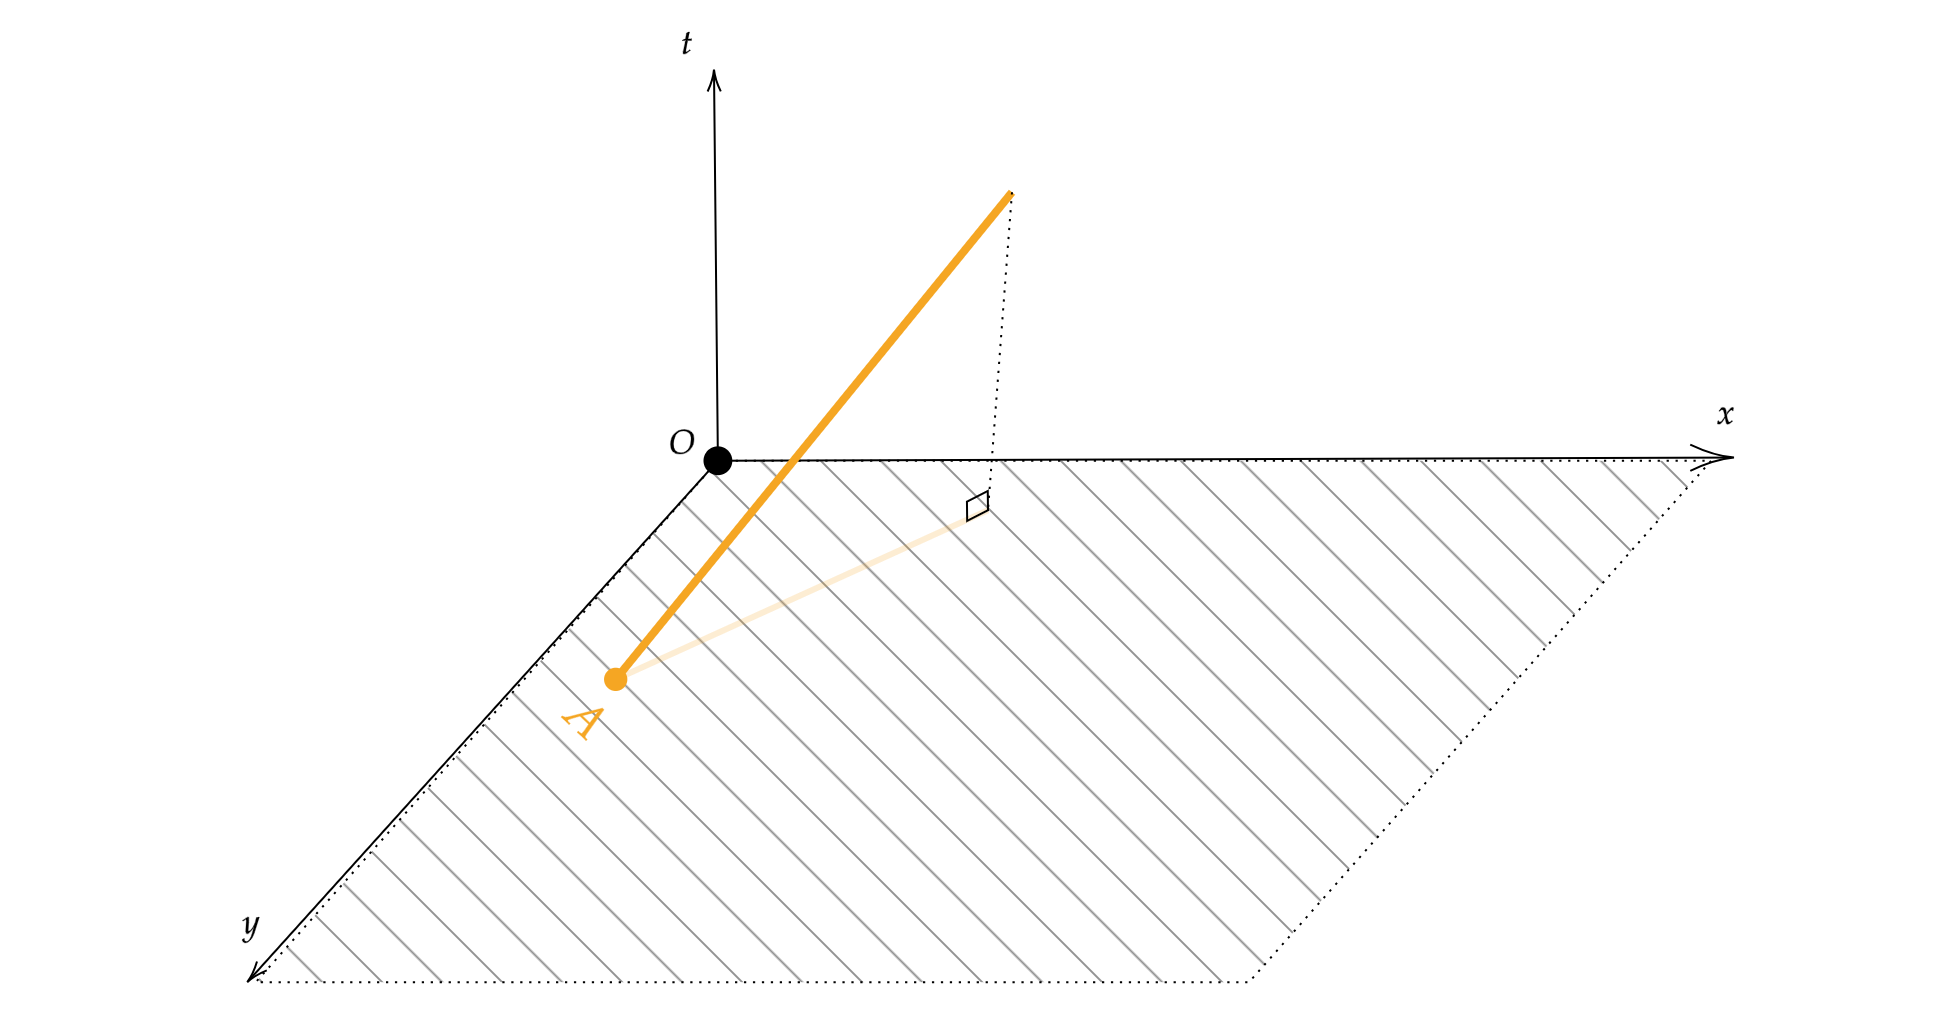
\includegraphics[scale = 0.25]{Problem_1/Image/Cach 1_A.png}
\captionsetup{justification=centering}
\caption{Đồ thị tọa độ-thời gian của bạn A \\
Quỹ đạo của bạn cũng chính là hình chiếu của đồ thị lên hệ trục Oxy!}
\end{figure}

\textit{Mỗi điểm giao nhau của các đường thẳng này biểu thị cho một lần gặp nhau}.

Từ các giao điểm thể hiện lần gặp mặt của A với B, A với C và B với C ta có thể lập \textit{một mặt phẳng} chứa cả ba đường thẳng của A, B và C. Do đường thẳng của D giao A và B nên \textit{cũng nằm trên mặt phẳng này}. 
Vì các đường thẳng \textit{đồng phẳng và không song song} nên đường thẳng của D và C sẽ giao nhau. \textit{Do đó bạn C và bạn D sẽ gặp nhau}.

\begin{figure}[H]
\centering
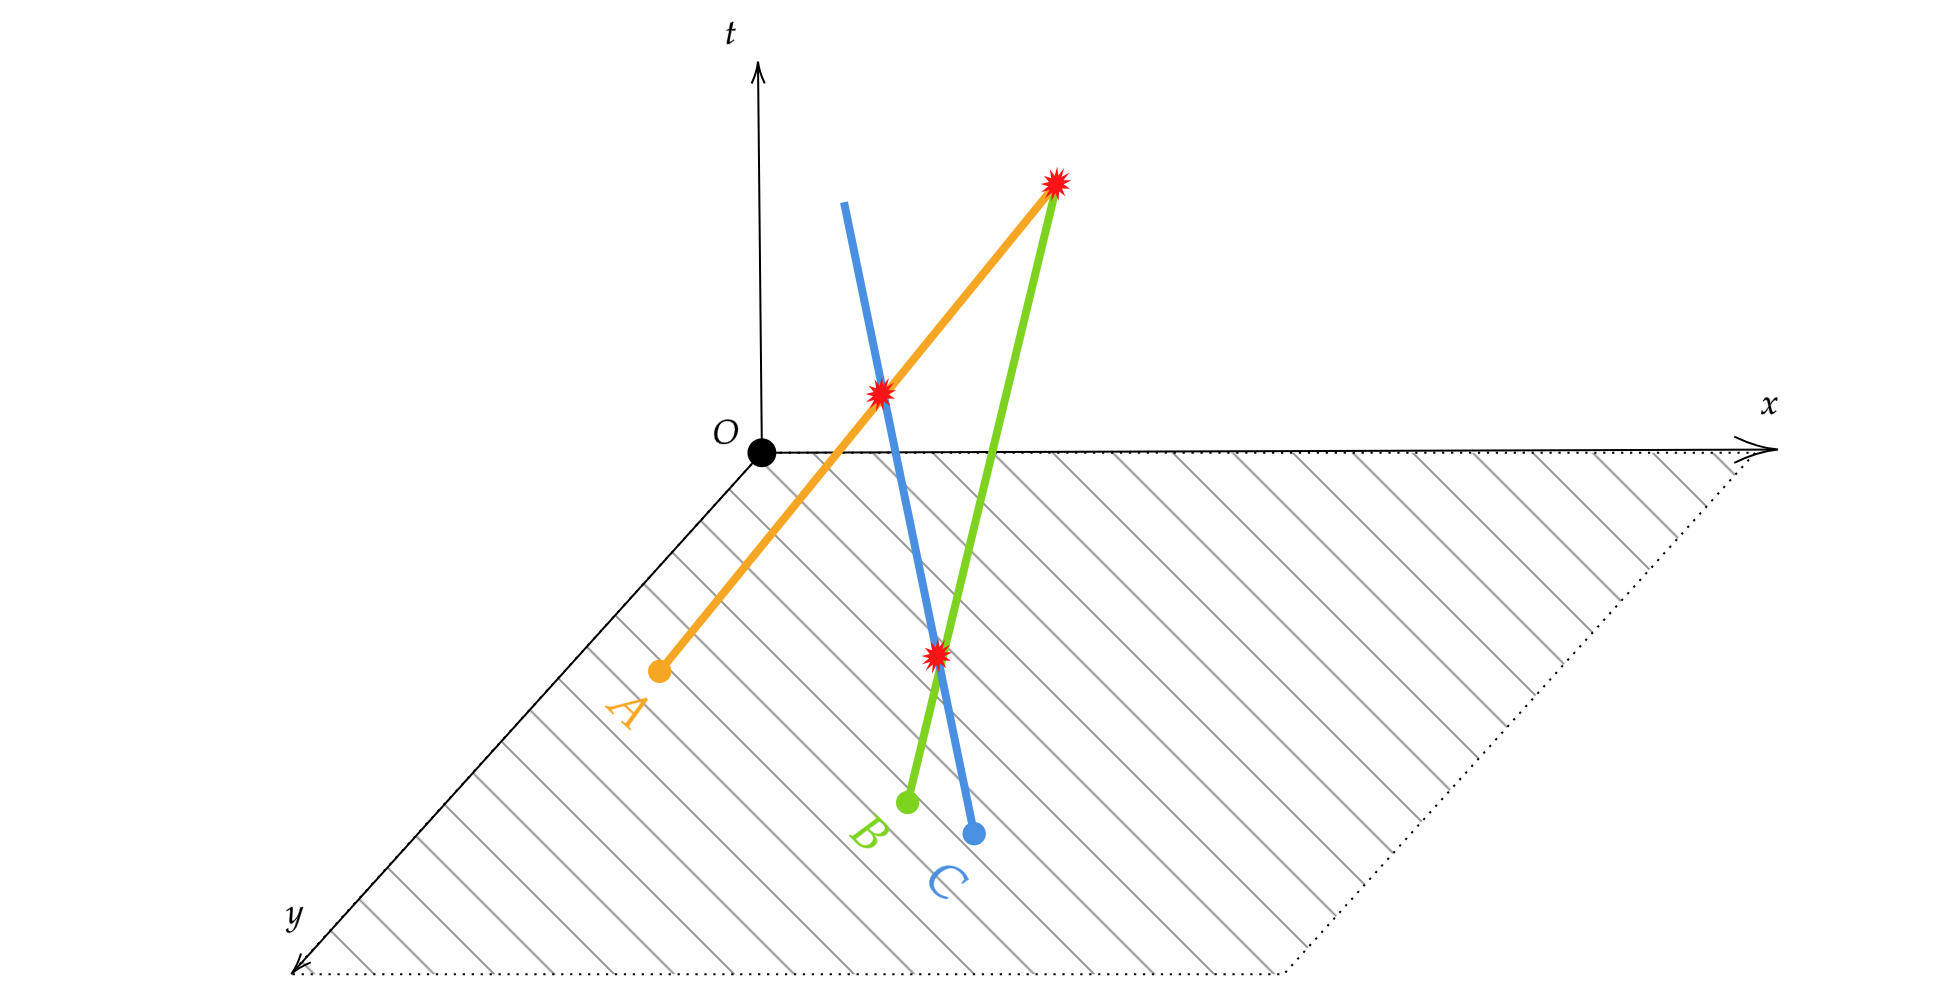
\includegraphics[scale = 0.25]{Problem_1/Image/Cach 1_B1.png}
\caption{Đồ thị tọa độ-thời gian của bạn A, B và C cùng nằm trên một mặt phẳng}
\end{figure}
\begin{figure}[H]
\centering
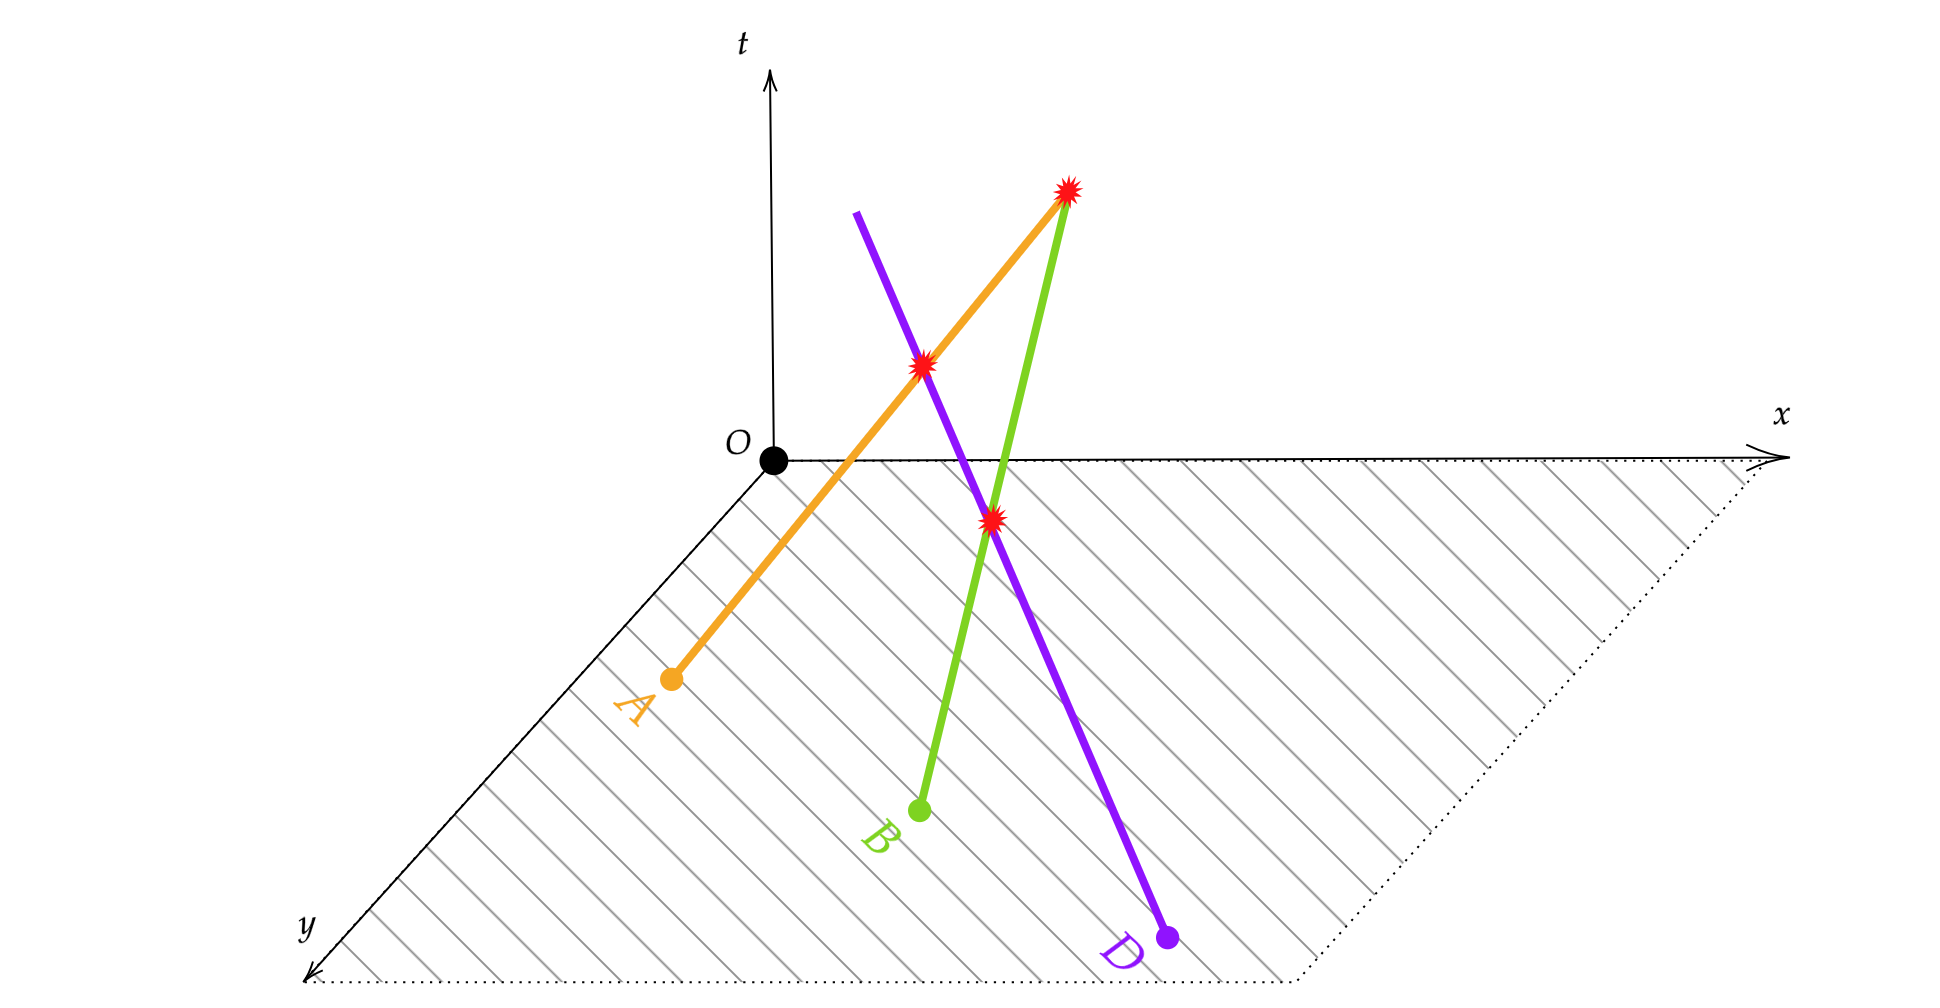
\includegraphics[scale = 0.25]{Problem_1/Image/Cach 1_B2.png}
\caption{Đồ thị của A, B và D cũng nằm trên một mặt phẳng}
\end{figure}
\begin{figure}[H]
\centering
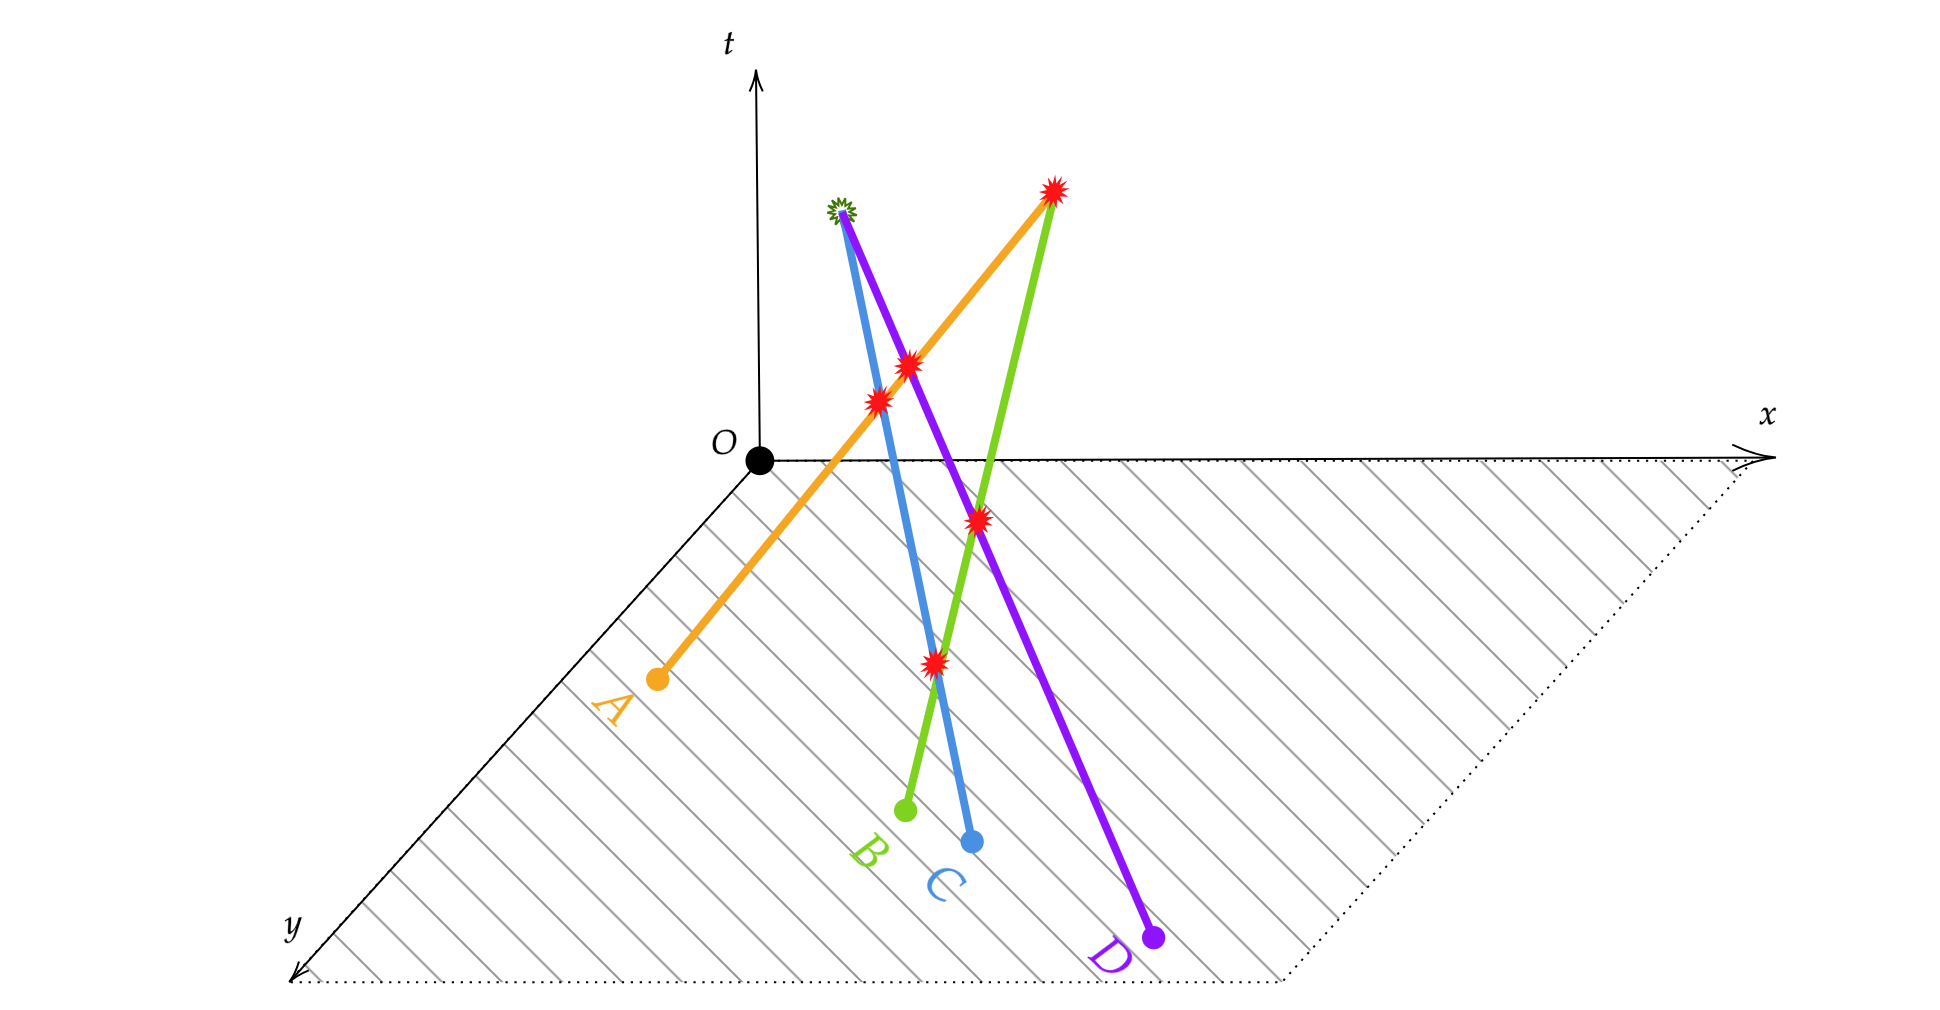
\includegraphics[scale = 0.25]{Problem_1/Image/Cach 1_B3.png}
\caption{Đồ thị của 4 bạn đồng phẳng}
\end{figure}

Vậy trường hợp gặp nhau thứ 6 chắc chắn sẽ xảy ra.\\

\textbf{Cách 2: Dùng hệ quy chiếu:}

Chọn hệ quy chiếu gắn với A, khi này, các đường thẳng quỹ đạo của B, C và D \textit{đều giao nhau tại điểm A} do cả ba bạn đã gặp A. Vì B đã gặp C nên quỹ đạo của B và C giao nhau, mà hai đường thẳng quỹ đạo này cũng giao nhau tại A nên quỹ đạo của B và C \textit{trùng nhau}. Tương tự, ta có đường thẳng quỹ đạo của B và D cũng trùng nhau. \textit{Do đó quỹ đạo của B, C và D trùng nhau}.

\begin{figure}[H]
\centering

\includegraphics[scale = 0.3]{Problem_1/Image/Cach 2.png}
\caption{Chuyển động của các bạn trong hệ quy chiếu gắn với A}
\end{figure}


Vận tốc của các bạn đối với mặt đất \textit{khác nhau và không đổi} nên vận tốc của những bạn còn lại đối với A cũng \textit{khác nhau và không đổi}.

Vì bạn C và bạn D chuyển động đều với vận tốc khác nhau trên \textit{cùng một đường thẳng}, sẽ có một lúc nào đó hai bạn đi qua nhau (nếu hai bạn chuyển động ngược chiều nhau) hoặc bạn này vượt qua bạn kia (nếu hai bạn chuyển động cùng chiều).

Vậy trường hợp gặp nhau thứ 6 chắc chắn sẽ xảy ra.

\textbf{Cách 3: (Lời giải của Murasakiiro)}

Giả sử các bạn gặp nhau tại các thời điểm $t_1, t_2, t_3, t_4, t_5$ như hình. Gọi $\Vec{r_A}, \Vec{r_B}, \Vec{r_C}, \Vec{r_D}$ là toạ độ ban đầu của các bạn $A, B, C, D$, với gốc toạ độ $O$ tuỳ ý.

\begin{center}
    \scalebox{0.8}{
        


\tikzset{every picture/.style={line width=0.75pt}} %set default line width to 0.75pt        

\begin{tikzpicture}[x=0.75pt,y=0.75pt,yscale=-1,xscale=1]
%uncomment if require: \path (0,11143); %set diagram left start at 0, and has height of 11143

%Straight Lines [id:da4257880873279283] 
\draw  [dash pattern={on 0.84pt off 2.51pt}]  (251.22,4004.97) -- (158.26,4227.86) ;
\draw [shift={(158.26,4227.86)}, rotate = 112.64] [color={rgb, 255:red, 0; green, 0; blue, 0 }  ][fill={rgb, 255:red, 0; green, 0; blue, 0 }  ][line width=0.75]      (0, 0) circle [x radius= 3.35, y radius= 3.35]   ;
%Straight Lines [id:da9952714607108861] 
\draw  [dash pattern={on 0.84pt off 2.51pt}]  (223.63,4015.45) -- (315.21,4249.92) ;
\draw [shift={(315.21,4249.92)}, rotate = 68.66] [color={rgb, 255:red, 0; green, 0; blue, 0 }  ][fill={rgb, 255:red, 0; green, 0; blue, 0 }  ][line width=0.75]      (0, 0) circle [x radius= 3.35, y radius= 3.35]   ;
%Straight Lines [id:da9393707554836688] 
\draw  [dash pattern={on 0.84pt off 2.51pt}]  (99.5,4115.86) -- (360.45,4188.13) ;
\draw [shift={(360.45,4188.13)}, rotate = 15.48] [color={rgb, 255:red, 0; green, 0; blue, 0 }  ][fill={rgb, 255:red, 0; green, 0; blue, 0 }  ][line width=0.75]      (0, 0) circle [x radius= 3.35, y radius= 3.35]   ;
%Straight Lines [id:da4242707810533324] 
\draw  [dash pattern={on 0.84pt off 2.51pt}]  (100.05,4125.24) -- (373.14,4119.72) ;
\draw [shift={(373.14,4119.72)}, rotate = 358.84] [color={rgb, 255:red, 0; green, 0; blue, 0 }  ][fill={rgb, 255:red, 0; green, 0; blue, 0 }  ][line width=0.75]      (0, 0) circle [x radius= 3.35, y radius= 3.35]   ;
%Straight Lines [id:da5822274503273119] 
\draw [color={rgb, 255:red, 126; green, 211; blue, 33 }  ,draw opacity=1 ][line width=3]    (315.21,4249.92) -- (298.09,4206.13) ;
\draw [shift={(295.9,4200.55)}, rotate = 68.64] [fill={rgb, 255:red, 126; green, 211; blue, 33 }  ,fill opacity=1 ][line width=0.08]  [draw opacity=0] (16.97,-8.15) -- (0,0) -- (16.97,8.15) -- cycle    ;
\draw [shift={(315.21,4249.92)}, rotate = 248.64] [color={rgb, 255:red, 126; green, 211; blue, 33 }  ,draw opacity=1 ][fill={rgb, 255:red, 126; green, 211; blue, 33 }  ,fill opacity=1 ][line width=3]      (0, 0) circle [x radius= 6.37, y radius= 6.37]   ;
%Straight Lines [id:da051074197187332526] 
\draw [color={rgb, 255:red, 245; green, 166; blue, 35 }  ,draw opacity=1 ][line width=3]    (158.26,4227.86) -- (176.09,4184.85) ;
\draw [shift={(178.39,4179.31)}, rotate = 112.53] [fill={rgb, 255:red, 245; green, 166; blue, 35 }  ,fill opacity=1 ][line width=0.08]  [draw opacity=0] (16.97,-8.15) -- (0,0) -- (16.97,8.15) -- cycle    ;
\draw [shift={(158.26,4227.86)}, rotate = 292.53] [color={rgb, 255:red, 245; green, 166; blue, 35 }  ,draw opacity=1 ][fill={rgb, 255:red, 245; green, 166; blue, 35 }  ,fill opacity=1 ][line width=3]      (0, 0) circle [x radius= 6.37, y radius= 6.37]   ;
%Straight Lines [id:da17569860173881802] 
\draw [color={rgb, 255:red, 74; green, 144; blue, 226 }  ,draw opacity=1 ][line width=3]    (360.45,4188.13) -- (324.86,4178.41) ;
\draw [shift={(319.07,4176.82)}, rotate = 15.29] [fill={rgb, 255:red, 74; green, 144; blue, 226 }  ,fill opacity=1 ][line width=0.08]  [draw opacity=0] (16.97,-8.15) -- (0,0) -- (16.97,8.15) -- cycle    ;
\draw [shift={(360.45,4188.13)}, rotate = 195.29] [color={rgb, 255:red, 74; green, 144; blue, 226 }  ,draw opacity=1 ][fill={rgb, 255:red, 74; green, 144; blue, 226 }  ,fill opacity=1 ][line width=3]      (0, 0) circle [x radius= 6.37, y radius= 6.37]   ;
%Straight Lines [id:da02986144608238317] 
\draw [color={rgb, 255:red, 144; green, 19; blue, 254 }  ,draw opacity=1 ][line width=3]    (373.14,4119.72) -- (308.52,4120.98) ;
\draw [shift={(302.52,4121.1)}, rotate = 358.88] [fill={rgb, 255:red, 144; green, 19; blue, 254 }  ,fill opacity=1 ][line width=0.08]  [draw opacity=0] (16.97,-8.15) -- (0,0) -- (16.97,8.15) -- cycle    ;
\draw [shift={(373.14,4119.72)}, rotate = 178.88] [color={rgb, 255:red, 144; green, 19; blue, 254 }  ,draw opacity=1 ][fill={rgb, 255:red, 144; green, 19; blue, 254 }  ,fill opacity=1 ][line width=3]      (0, 0) circle [x radius= 6.37, y radius= 6.37]   ;
%Shape: Star [id:dp4652455317009081] 
\draw  [draw opacity=0][fill={rgb, 255:red, 208; green, 2; blue, 27 }  ,fill opacity=1 ] (202.25,4118.9) -- (202.76,4120.88) -- (204.24,4119.34) -- (203.67,4121.31) -- (205.77,4120.56) -- (204.25,4122.07) -- (206.5,4122.29) -- (204.38,4122.99) -- (206.25,4124.13) -- (204.01,4123.85) -- (205.09,4125.65) -- (203.25,4124.47) -- (203.28,4126.51) -- (202.25,4124.69) -- (201.23,4126.51) -- (201.26,4124.47) -- (199.42,4125.65) -- (200.49,4123.85) -- (198.26,4124.13) -- (200.13,4122.99) -- (198.01,4122.29) -- (200.25,4122.07) -- (198.73,4120.56) -- (200.84,4121.31) -- (200.27,4119.34) -- (201.74,4120.88) -- cycle ;
%Shape: Star [id:dp17943360623521842] 
\draw  [draw opacity=0][fill={rgb, 255:red, 208; green, 2; blue, 27 }  ,fill opacity=1 ] (131.08,4120.55) -- (131.6,4122.54) -- (133.07,4120.99) -- (132.5,4122.97) -- (134.6,4122.22) -- (133.08,4123.73) -- (135.33,4123.95) -- (133.21,4124.64) -- (135.08,4125.78) -- (132.84,4125.51) -- (133.92,4127.3) -- (132.08,4126.12) -- (132.11,4128.16) -- (131.08,4126.34) -- (130.06,4128.16) -- (130.09,4126.12) -- (128.25,4127.3) -- (129.33,4125.51) -- (127.09,4125.78) -- (128.96,4124.64) -- (126.84,4123.95) -- (129.09,4123.73) -- (127.57,4122.22) -- (129.67,4122.97) -- (129.1,4120.99) -- (130.57,4122.54) -- cycle ;
%Shape: Star [id:dp03789410132743454] 
\draw  [draw opacity=0][fill={rgb, 255:red, 208; green, 2; blue, 27 }  ,fill opacity=1 ] (265.15,4118.34) -- (265.66,4120.33) -- (267.13,4118.79) -- (266.56,4120.76) -- (268.67,4120.01) -- (267.15,4121.52) -- (269.39,4121.74) -- (267.27,4122.44) -- (269.14,4123.57) -- (266.91,4123.3) -- (267.98,4125.1) -- (266.14,4123.92) -- (266.17,4125.96) -- (265.15,4124.14) -- (264.12,4125.96) -- (264.15,4123.92) -- (262.31,4125.1) -- (263.39,4123.3) -- (261.15,4123.57) -- (263.02,4122.44) -- (260.9,4121.74) -- (263.15,4121.52) -- (261.63,4120.01) -- (263.73,4120.76) -- (263.16,4118.79) -- (264.64,4120.33) -- cycle ;
%Shape: Star [id:dp6092374284959783] 
\draw  [draw opacity=0][fill={rgb, 255:red, 208; green, 2; blue, 27 }  ,fill opacity=1 ] (193.98,4138.2) -- (194.49,4140.19) -- (195.96,4138.65) -- (195.4,4140.62) -- (197.5,4139.87) -- (195.98,4141.38) -- (198.22,4141.6) -- (196.1,4142.3) -- (197.98,4143.44) -- (195.74,4143.16) -- (196.81,4144.96) -- (194.97,4143.78) -- (195,4145.82) -- (193.98,4144) -- (192.95,4145.82) -- (192.98,4143.78) -- (191.14,4144.96) -- (192.22,4143.16) -- (189.98,4143.44) -- (191.86,4142.3) -- (189.73,4141.6) -- (191.98,4141.38) -- (190.46,4139.87) -- (192.56,4140.62) -- (191.99,4138.65) -- (193.47,4140.19) -- cycle ;
%Shape: Star [id:dp9525934681135235] 
\draw  [draw opacity=0][fill={rgb, 255:red, 208; green, 2; blue, 27 }  ,fill opacity=1 ] (282.8,4161.93) -- (283.31,4163.91) -- (284.79,4162.37) -- (284.22,4164.34) -- (286.32,4163.6) -- (284.8,4165.1) -- (287.05,4165.32) -- (284.92,4166.02) -- (286.8,4167.16) -- (284.56,4166.89) -- (285.64,4168.68) -- (283.79,4167.5) -- (283.82,4169.54) -- (282.8,4167.72) -- (281.78,4169.54) -- (281.81,4167.5) -- (279.97,4168.68) -- (281.04,4166.89) -- (278.8,4167.16) -- (280.68,4166.02) -- (278.56,4165.32) -- (280.8,4165.1) -- (279.28,4163.6) -- (281.38,4164.34) -- (280.81,4162.37) -- (282.29,4163.91) -- cycle ;
%Shape: Star [id:dp7689921001871347] 
\draw  [color={rgb, 255:red, 65; green, 117; blue, 5 }  ,draw opacity=1 ][line width=0.75]  (234.6,4034.49) -- (235.53,4038.11) -- (238.22,4035.29) -- (237.18,4038.89) -- (241.01,4037.52) -- (238.24,4040.27) -- (242.33,4040.67) -- (238.47,4041.94) -- (241.88,4044.01) -- (237.81,4043.52) -- (239.77,4046.78) -- (236.41,4044.63) -- (236.47,4048.35) -- (234.6,4045.04) -- (232.74,4048.35) -- (232.79,4044.63) -- (229.44,4046.78) -- (231.4,4043.52) -- (227.32,4044.01) -- (230.74,4041.94) -- (226.87,4040.67) -- (230.96,4040.27) -- (228.19,4037.52) -- (232.02,4038.89) -- (230.98,4035.29) -- (233.67,4038.11) -- cycle ;

% Text Node
\draw (146.27,4236.75) node [anchor=north west][inner sep=0.75pt]   [align=left] {$\displaystyle \textcolor[rgb]{0.96,0.65,0.14}{A}$};
% Text Node
\draw (321.83,4240.13) node [anchor=north west][inner sep=0.75pt]   [align=left] {$\displaystyle \textcolor[rgb]{0.49,0.83,0.13}{B}$};
% Text Node
\draw (368.42,4177.79) node [anchor=north west][inner sep=0.75pt]   [align=left] {$\displaystyle \textcolor[rgb]{0.29,0.56,0.89}{C}$};
% Text Node
\draw (379.64,4108.83) node [anchor=north west][inner sep=0.75pt]   [align=left] {$\displaystyle \textcolor[rgb]{0.56,0.07,1}{D}$};
% Text Node
\draw (262,4164) node [anchor=north west][inner sep=0.75pt]   [align=left] {$\displaystyle t_{1}$};
% Text Node
\draw (262,4088) node [anchor=north west][inner sep=0.75pt]   [align=left] {$\displaystyle t_{2}$};
% Text Node
\draw (182,4094) node [anchor=north west][inner sep=0.75pt]   [align=left] {$\displaystyle t_{3}$};
% Text Node
\draw (169,4139) node [anchor=north west][inner sep=0.75pt]   [align=left] {$\displaystyle t_{4}$};
% Text Node
\draw (112,4098) node [anchor=north west][inner sep=0.75pt]   [align=left] {$\displaystyle t_{5}$};
% Text Node
\draw (248,4030) node [anchor=north west][inner sep=0.75pt]   [align=left] {$\displaystyle \textcolor[rgb]{0.25,0.46,0.02}{t_{6}}$};


\end{tikzpicture}
    }
\end{center}
Với $5$ cặp gặp nhau, ta có điều kiện gặp của $5$ cặp điểm này là:
\begin{align*}
\left\{
    \begin{array}{rrrr}
    \left(\Vec{r_B} - \Vec{r_C} \right)   & = & t_1 \left( \Vec{v_B} - \Vec{v_C} \right) & \text{(cặp B-C).} \\
    \left(\Vec{r_B} - \Vec{r_D} \right)   & = & t_2 \left( \Vec{v_B} - \Vec{v_D} \right) & \text{(cặp B-D).} \\
    \left(\Vec{r_A} - \Vec{r_D} \right)   & = & t_3 \left( \Vec{v_A} - \Vec{v_D} \right) & \text{(cặp A-D).} \\
    \left(\Vec{r_C} - \Vec{r_A} \right)   & = & t_4 \left( \Vec{v_C} - \Vec{v_A} \right) & \text{(cặp C-A).} \\
    \left(\Vec{r_C} - \Vec{r_D} \right)   & = & t_5 \left( \Vec{v_C} - \Vec{v_D} \right) & \text{(cặp D-C).} \\
    \end{array}
\right.
\end{align*}
Từ hệ phương trình trên, ta khử $\Vec{r_C}, \Vec{r_D}, \Vec{v_C}, \Vec{v_D}$ ta sẽ thu được phương trình sau:
\begin{align}
    \Vec{r_A} - \Vec{r_B} & =  \frac{t_1 t_2 \left(t_4 - t_3 \right) + t_2 t_4 \left( t_3 - t_5 \right) +t_1 t_3 \left(t_5 - t_4 \right)}{t_5 \left( t_1 + t_3 - t_2 - t_4 \right) - t_1 t_3 - t_2 t_4} \left( \Vec{v_A} - \Vec{v_B} \right) = t_6 \left( \Vec{v_A} - \Vec{v_B} \right).
    \label{S2_eq.1.1}
\end{align}
Như vậy từ biểu thức (\ref{S2_eq.1.1}) ta thấy rằng cặp điểm $\left(A-B\right)$ có va chạm nhau. Như vậy có $6$ va chạm diễn ra.
\item 
\begin{figure}[ht]
    \centering
    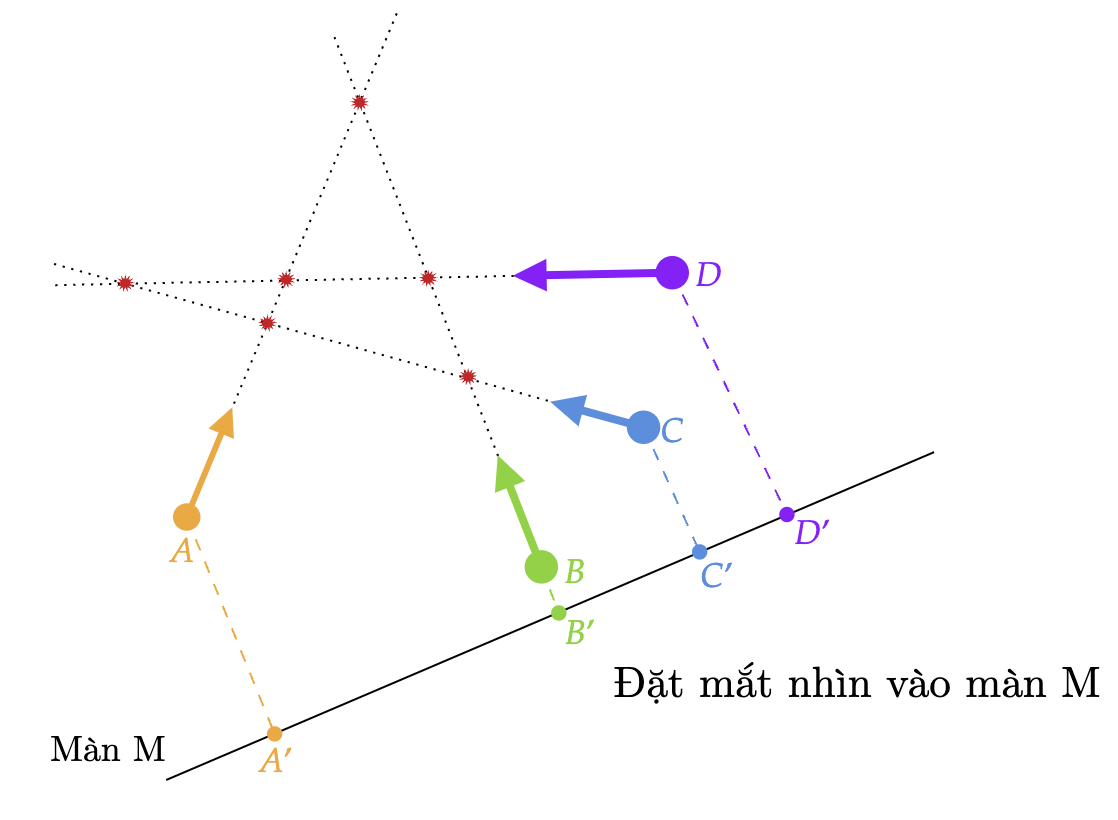
\includegraphics[scale=0.45]{Problem_1/Image/S2.2.1.png}
    \caption{}
    \label{S2.2.1}
\end{figure}

Ta sẽ biến một hệ 2D thành một hệ 1D bằng hình (\ref{S2.2.1}). Một số điểm cần lưu ý:
\begin{enumerate}
    \item Do các bạn đều va chạm mỗi khi đi va điểm giao nhau của 2 quỹ đạo. Nên khi hình ảnh hai bạn trùng nhau trên màn tương đương hai bạn va chạm.
    \item Hành động va chạm vẫn tuân theo quy tắc mà đề bài đã đề ra là trao đổi tốc độ và quỹ đạo.
\end{enumerate}
{ \textbf{Tổng va chạm diễn ra}}

Hình (\ref{S2.2.2}) mô tả hai trường hợp. Nếu \textit{không phân biệt} rõ hạt $C'$ hay hạt $D'$ thì giống như hai hạt \textit{đi xuyên qua nhau mà không tương tác gì}. 
\begin{figure}[ht]
    \centering
    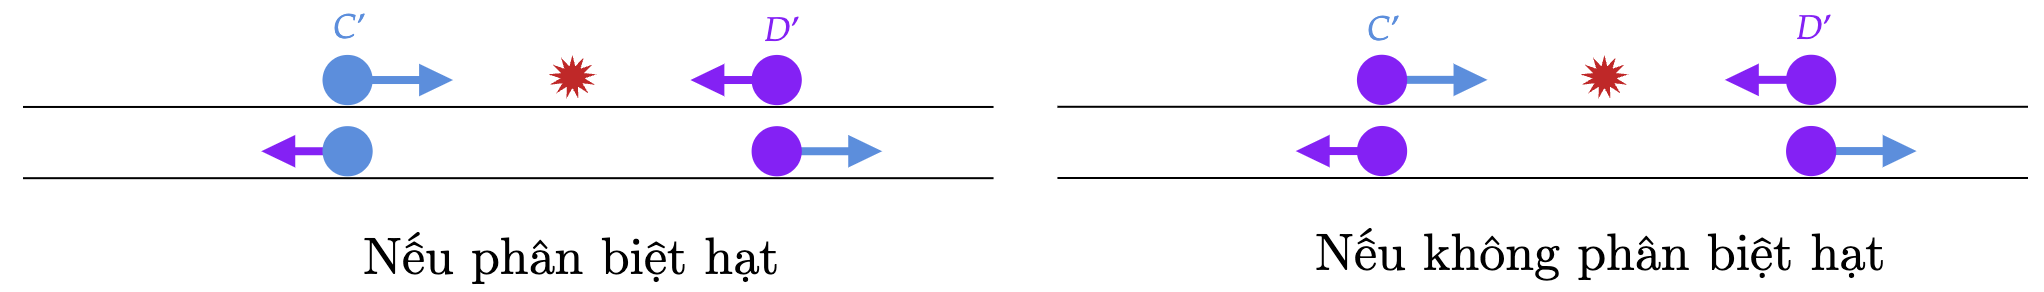
\includegraphics[scale=0.45]{Problem_1/Image/S2.2.2.png}
    \caption{}
    \label{S2.2.2}
\end{figure}
\\
Vậy lúc này nếu nói về số va chạm tổng cộng thì phần 2 vẫn có hiện tượng giống như phần 1. Như vậy tổng số va chạm diễn ra vẫn là \textbf{6}.

\textit{Đến đây ta vô tình bổ sung thêm cho nhận định 1 trong phần lưu ý.}

{ \textbf{Phân loại loại hạt trên màn.}}
\\Từ giờ để dễ gọi, ta sẽ thay thế từ `\textit{bạn}' thành `\textit{hạt}'. 

Lúc này thì bài toán đã trở thành một bài toán va chạm 1D. Các vận tốc của các hạt là bất kì, nhưng vẫn thoả mãn điều kiện ở Phần 1.
\begin{figure}[ht]
    \centering
    
\includegraphics[scale=0.6]{Problem_1/Image/S2.2.3.png}
    \caption{}
    \label{S2.2.3}
\end{figure}
\\
Từ đây ta chia các hạt trên màn gồm: \textbf{hạt ngoài rìa} ($A'$ và $D'$) và \textbf{hạt bên trong} ($B'$ và $C'$).

Lý do để chia cũng khá dễ hiểu, ta thấy rằng tiềm năng để hạt ngoài rìa va chạm ít hơn so với lại hạt bên trong. Hạt ngoài rìa tự do một đầu, nên khả năng thoát khỏi hệ sớm hơn hạt bên trong. Giờ ta sẽ đi khảo sát số va chạm của các loại hạt này.

\textbf{Hạt ngoài rìa:}

Để số va chạm có thể được tối đa thì

\textit{Điều kiện 1}: Tất các hạt phải \textit{hướng vận tốc về phía hạt $D'$}. Lý do là vì để cho hạt $D'$ có khả năng trao đổi vận tốc với hạt đó. Vì vậy số va chạm lớn nhất của $D'$ diễn ra khi các hạt đều hướng về phía $D'$.
\begin{figure}[ht]
    \centering
    
\includegraphics[scale=0.6]{Problem_1/Image/S2.2.4.png}
    \caption{}
    \label{S2.2.4}
\end{figure}

\textit{Điều kiện 2:} Hạt $D'$ phải va chạm với những hạt có tốc độ thấp và lần lượt đến các hạt có tốc độ cao sau. Bởi vì nếu hạt $C'$ đuổi theo hạt $D'$, mà tốc độ của $C'$ nhỏ hơn của $D'$ thì hạt $D'$ sẽ thoát khỏi hệ và kết thúc quá trình va chạm. Vì thế mình chia các loại tốc độ thành: \textit{Lớn-Trung-Nhỏ}

\begin{center}
\begin{tabular}{|l|c|}
\hline
Thứ tự va chạm    & Số va chạm của $D'$ \\ \hline
Lớn               & 1                   \\ \hline
Trung(Nhỏ) - Lớn  & 2                   \\ \hline
Nhỏ - Trung - Lớn & 3                   \\ \hline
\end{tabular}
\end{center}


Nhìn vào bảng thì ta thấy số va chạm khả dĩ của hạt ngoài rìa là \textbf{[1;3]}.

\textbf{Hạt bên trong:}
\\
Ta sẽ lấy đại diện là hạt $B'$. Dựa vào kết quả đã được tính ở những hạt ngoài rìa, ta lập luận được số va chạm mà \textit{không có sự góp mặt của $D'$} là \textbf{[3;5]}. Lý do là bởi tổng số va chạm vẫn bảo toàn là \textbf{6}.

Các hạt $A'$ và $C'$ không thể va chạm trực tiếp với nhau. Lý do là vì khi $C'$ gặp $B'$ thì đã bị bật ra do va chạm đàn hồi. Tương tự với $A'$. Vì thế nên sẽ không có va chạm giữa $A'$ và $C'$, số va chạm là $0$.


\begin{figure}[ht]
    \centering
    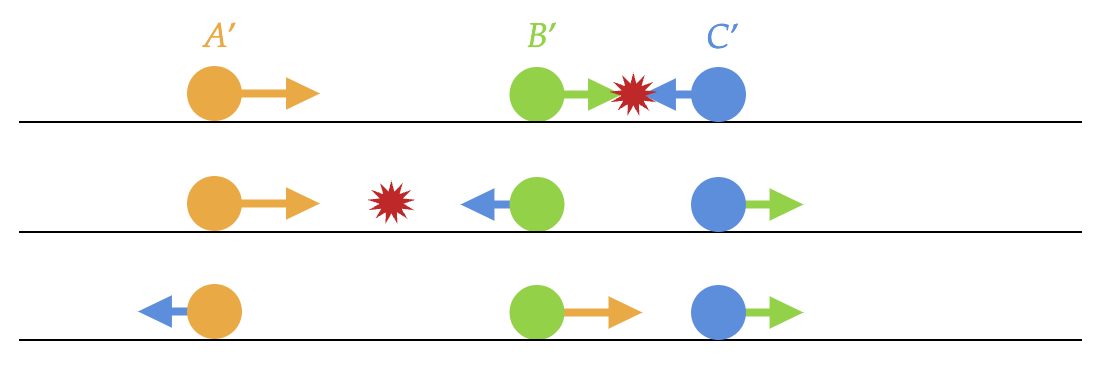
\includegraphics[scale=0.6]{Problem_1/Image/S2.2.5.png}
    \caption{Tương tác của $A'-B'-C'$}
    \label{S2.2.5}
\end{figure}

Do số va chạm của các hạt còn lại (là $A'$, $B'$, $C'$) gồm va chạm giữa $B'-C'$, $B'-A'$ (cặp $A'-C'$ không thể xảy ra va chạm như vừa chứng minh). Chung quy đều là va chạm có mặt $B'$. Như vậy số va chạm mà $B'$ trải nghiệm thuộc \textbf{[3;5]}.

 \textbf{Tổng kết}
\\
\begin{center}
    \begin{tabular}{|l|c|}
\hline
              & Số va chạm khả dĩ                   \\ \hline
Hạt ngoài rìa & \textbf{[1;3]} \\ \hline
Hạt bên trong & \textbf{[3;5]} \\ \hline
\end{tabular}
\end{center}
Từ đây dễ dàng kết luận là số va chạm lớn nhất một hạt (bạn) có thể trải nghiệm là \textbf{5}.
\item \textbf{Phổ điểm}

\begin{center}

\begin{tabular}{|c|p{3.5cm}|p{7.5cm}|c|}
\hline
\multicolumn{1}{|l|}{Phần} &
  \multicolumn{2}{l|}{Nội dung} &
  \multicolumn{1}{l|}{Điểm thành phần} \\ \hline
\multirow{6}{*}{1} &
  \multicolumn{1}{l|}{\multirow{3}{*}{Nếu làm theo cách 1}} &
  Biểu diễn chuyển động trên trục Oxyt. &
  0.5 \\ \cline{3-4} 
                   & \multicolumn{1}{l|}{} & Biện luận 3 đồ thị bất kì đồng phẳng.         & 1    \\ \cline{3-4} 
 &
  \multicolumn{1}{l|}{} &
  Kết luận 4 đồ thị đồng phẳng, suy ra có cuộc gặp nhau thứ 6. &
  0.5 \\ \cline{2-4} 
 &
  \multicolumn{1}{l|}{\multirow{3}{*}{Nếu làm theo cách 2}} &
  Biện luận chuyển động trong hệ quy chiếu gắn với một người. &
  0.5 \\ \cline{3-4} 
                   & \multicolumn{1}{l|}{} & Biện luận các đường thẳng quỹ đạo trùng nhau. & 1    \\ \cline{3-4} 
                   & \multicolumn{1}{l|}{} & Kết luận cuộc gặp nhau thứ 6 có xảy ra.       & 0.5  \\ \hline
\multirow{7}{*}{2} & \multicolumn{2}{l|}{Tương đương hệ 2D và 1D.}                                            & 0.5 \\ \cline{2-4} 
                   & \multicolumn{2}{l|}{Chứng minh tổng số va chạm.}                      & 0.25 \\ \cline{2-4} 
                   & \multicolumn{2}{l|}{Điều kiện 1: Hạt ngoài rìa.}                      & 0.25  \\ \cline{2-4} 
                   & \multicolumn{2}{l|}{Điều kiện 2: Hạt ngoài rìa.}                      & 0.25 \\ \cline{2-4} 
                   & \multicolumn{2}{l|}{Va chạm khả dĩ hạt ngoài rìa.}                    & 0.25 \\ \cline{2-4} 
                   & \multicolumn{2}{l|}{Chứng minh cặp hạt A-C không va chạm.}            & 0.25 \\ \cline{2-4} 
                   & \multicolumn{2}{l|}{Va chạm khả dĩ hạt bên trong.}                    & 0.25 \\ \hline
\end{tabular}

\end{center}
Nếu làm theo cách khác nhưng hợp lý thì được trọn điểm.
\end{enumerate}

\newpage
{\normalcolor \textbf{CÂU 2 (4 điểm)}}\vspace{1.5mm}

\setcounter{equation}{0}
\begin{figure}[ht]
\centering
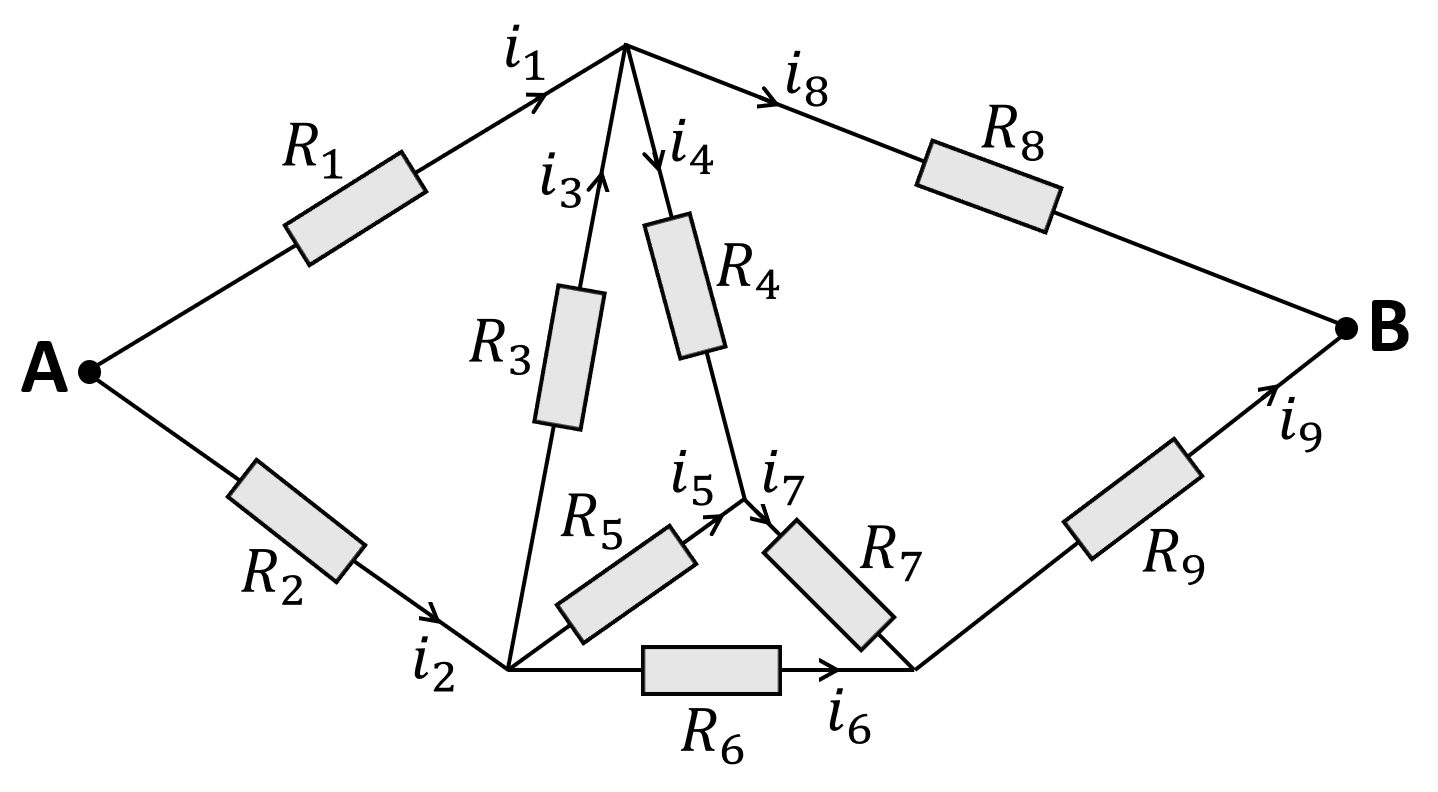
\includegraphics[width=0.6\textwidth,keepaspectratio]{Problem_2/Figs/P2A.png}
\end{figure}

Xét một mạch điện cấu tạo từ các điện trở $R_1$, $R_2$, ..., $R_8$, $R_9$. Khi đặt hiệu điện thế $1V$ vào hai đầu mạch A và B thì thu được phân bố dòng điện với chiều đi như hình vẽ, cường độ đo được theo đơn vị $mA$ là:
\begin{equation}
i_1 = 33 \ , \ i_2 = 28 \ , \ i_3 = 5 \ , \ i_4 = 2 \ , \ i_5 = 7 \ , \ i_6 = 16 \ , \ i_7 = 9 \ , \ i_8 = 36 \ , \ i_9 = 25 \ . \nonumber
\end{equation}
Với những thông tin đã cho thì liệu có thể xác định được giá trị của các điện trở hay không, và nếu có thì hãy xác định $R_1$ và $R_9$.
\setcounter{equation}{0}
\begin{center}
    \normalcolor{\textbf{Bài giải}}
\end{center}
\begin{enumerate}
    \item \textbf{Ổn định nhiệt độ tại động cơ:} Để nhiệt độ của động cơ ổn định, chất tải nhiệt ở vòng 1 phải thu nhiệt từ động cơ cũng với công suất $\mathcal{P}$.

    \textbf{Ổn định nhiệt độ của chất tải nhiệt trong vòng 1:} Giả sử nhiệt độ cao nhất của chất tải nhiệt tại vòng 1 là $T_0$. Sau một khoảng thời gian $\Delta t$ nhỏ, có một lượng $L_1 \Delta t$ chất tải nhiệt ở vòng 1 đi tới buồng trao đổi nhiệt ở nhiệt độ $T_0$, $L_1 \Delta t$ ra khỏi buồng trao đổi nhiệt ở nhiệt độ $T$. Như vậy, nhiệt lượng mà chất tải nhiệt trong vòng 1 đã truyền cho chất tải nhiệt trong vòng 2 trong khoảng thời gian $\Delta t$ là:
    \begin{equation}
        \Delta Q= L_1 \Delta t C_1 T_0 - L_1 \Delta t C_1 T.
    \end{equation}
    Do đó công suất truyền nhiệt của vòng 1 cho vòng 2 là:
    \begin{equation}
        \mathcal{P'}=\dfrac{\Delta Q}{\Delta t}=L_1 C_1 (T_0-T).
    \end{equation}
    Để nhiệt độ của chất tải nhiệt trong vòng 1 là ổn định, nhiệt lượng nó thu từ động cơ trong một khoảng thời gian phải bằng nhiệt tỏa ra cho vòng 2 trong một thời gian tương ứng, nên $\mathcal{P'}=\mathcal{P}$. Ta nhận được biểu thức của $T_0$:
    \begin{equation}
        T_0=T+\dfrac{\mathcal{P}}{L_1 C_1}.
    \end{equation}

    \textbf{Ổn định nhiệt độ của chất tải nhiệt trong vòng 2:} Xét một lớp chất tải nhiệt trong vòng 1 tại buồng trao đổi nhiệt, do nhiệt độ của chất giảm tuyến tính dọc theo buồng, nên nhiệt lượng mà lớp chất đó nhận được từ lớp chất đằng sau nó trên một khoảng thời gian bằng với công suất nhiệt mà nó tỏa ra cho lớp chất đằng trước nó trên một khoảng thời gian tương ứng.

    \begin{figure}[!h]
        \centering
        \scalebox{1}{



% Gradient Info
  
\tikzset {_q77e6wcqi/.code = {\pgfsetadditionalshadetransform{ \pgftransformshift{\pgfpoint{0 bp } { 0 bp }  }  \pgftransformrotate{-90 }  \pgftransformscale{2 }  }}}
\pgfdeclarehorizontalshading{_fmzdny4at}{150bp}{rgb(0bp)=(1,0.2,0);
rgb(37.5bp)=(1,0.2,0);
rgb(62.5bp)=(0.31,0.9,0.9);
rgb(100bp)=(0.31,0.9,0.9)}
\tikzset{_hcup74vjq/.code = {\pgfsetadditionalshadetransform{\pgftransformshift{\pgfpoint{0 bp } { 0 bp }  }  \pgftransformrotate{-90 }  \pgftransformscale{2 } }}}
\pgfdeclarehorizontalshading{_6boflkrhi} {150bp} {color(0bp)=(transparent!25);
color(37.5bp)=(transparent!25);
color(62.5bp)=(transparent!25);
color(100bp)=(transparent!25) } 
\pgfdeclarefading{_hpd8pgkav}{\tikz \fill[shading=_6boflkrhi,_hcup74vjq] (0,0) rectangle (50bp,50bp); } 
\tikzset{every picture/.style={line width=0.75pt}} %set default line width to 0.75pt        

\begin{tikzpicture}[x=0.75pt,y=0.75pt,yscale=-1,xscale=1]
%uncomment if require: \path (0,300); %set diagram left start at 0, and has height of 300

%Shape: Rectangle [id:dp2185885188174972] 
\path  [shading=_fmzdny4at,_q77e6wcqi,path fading= _hpd8pgkav ,fading transform={xshift=2}] (270,71.6) -- (340,71.6) -- (340,219.6) -- (270,219.6) -- cycle ; % for fading 
 \draw  [color={rgb, 255:red, 0; green, 0; blue, 0 }  ,draw opacity=0 ] (270,71.6) -- (340,71.6) -- (340,219.6) -- (270,219.6) -- cycle ; % for border 

%Straight Lines [id:da0212006301849037] 
\draw [color={rgb, 255:red, 0; green, 0; blue, 0 }  ,draw opacity=1 ]    (270,70.6) -- (270,220.6) ;
%Straight Lines [id:da2341810130015769] 
\draw [color={rgb, 255:red, 0; green, 0; blue, 0 }  ,draw opacity=1 ]    (340,71.6) -- (340,220.6) ;
%Straight Lines [id:da12568741183524867] 
\draw [color={rgb, 255:red, 142; green, 23; blue, 40 }  ,draw opacity=1 ]   (360,68.6) -- (360,222.6) ;
\draw [shift={(360,224.6)}, rotate = 270] [color={rgb, 255:red, 142; green, 23; blue, 40 }  ,draw opacity=1 ][line width=0.75]    (10.93,-3.29) .. controls (6.95,-1.4) and (3.31,-0.3) .. (0,0) .. controls (3.31,0.3) and (6.95,1.4) .. (10.93,3.29)   ;
%Straight Lines [id:da8980559358913409] 
\draw [color={rgb, 255:red, 1; green, 0; blue, 0 }  ,draw opacity=1 ]   (306,84.6) -- (306,100.6) -- (306,123.6) ;
\draw [shift={(306,125.6)}, rotate = 270] [color={rgb, 255:red, 1; green, 0; blue, 0 }  ,draw opacity=1 ][line width=0.75]    (10.93,-3.29) .. controls (6.95,-1.4) and (3.31,-0.3) .. (0,0) .. controls (3.31,0.3) and (6.95,1.4) .. (10.93,3.29)   ;
%Straight Lines [id:da9368761284836362] 
\draw   [color={rgb, 255:red, 1; green, 0; blue, 0 }  ,draw opacity=1 ] (305,145.6) -- (305,161.6) -- (305,184.6) ;
\draw [shift={(305,186.6)}, rotate = 270] [color={rgb, 255:red, 1; green, 0; blue, 0 }  ][line width=0.75]    (10.93,-3.29) .. controls (6.95,-1.4) and (3.31,-0.3) .. (0,0) .. controls (3.31,0.3) and (6.95,1.4) .. (10.93,3.29)   ;
%Straight Lines [id:da4947984933205438] 
\draw [color={rgb, 255:red, 1; green, 0; blue, 0 }  ,draw opacity=1 ] [dash pattern={on 4.5pt off 4.5pt}]  (340,113.6) -- (270,113.6) ;
%Straight Lines [id:da4467544607652605] 
\draw [color={rgb, 255:red, 1; green, 0; blue, 0 }  ,draw opacity=1 ] [dash pattern={on 4.5pt off 4.5pt}]  (272,161.6) -- (289,161.6) -- (296,161.6) -- (342,161.6) ;

% Text Node
\draw (365,218) node [anchor=north west][inner sep=0.75pt]   [align=left] {$\displaystyle x$};
% Text Node
\draw (366,136) node [anchor=north west][inner sep=0.75pt]   [align=left] {$\displaystyle \boxed{T( x) =T( 0) -kx}$};
% Text Node
\draw (307,94) node [anchor=north west][inner sep=0.75pt]   [align=left] {$\displaystyle \textcolor[rgb]{0,0,0}{\mathcal{P}_{\text{vào}}}$};
% Text Node
\draw (307,164.6) node [anchor=north west][inner sep=0.75pt]   [align=left] {$\displaystyle \textcolor[rgb]{0,0,0}{\mathcal{P}_{\text{ra}}}$};
% Text Node
\draw (144,135) node [anchor=north west][inner sep=0.75pt]   [align=left] {$\displaystyle \boxed{\mathcal{P}_{\text{vào}} =\mathcal{P}_{\text{ra}} \sim k}$};


\end{tikzpicture}}
        \caption{Mô hình hóa sự truyền nhiệt}
        \label{fig:99}
    \end{figure}

    Như vậy, nguyên nhân làm giảm nhiệt độ của lớp chất đó chỉ là trao đổi nhiệt với chất tải nhiệt trong vòng 2, có nhiệt độ thấp hơn. Vì tiết diện buồng là đều, lưu lượng của dòng chất không đổi nên vận tốc chảy của chất tải nhiệt trong vòng 1 tại buồng trao đổi nhiệt là không đổi. Thế nên để nhiệt độ luôn giảm tuyến tính dọc theo buồng, công suất tỏa nhiệt tại mọi vị trí dọc theo buồng phải như nhau. Mà công suất tỏa nhiệt này lại tỉ lệ với độ chênh lệch nhiệt độ giữa chất tải nhiệt của hai vòng 1 và 2 tại điểm mà chúng tiếp xúc nhau, nên nhiệt độ của chất tải nhiệt trong vòng 2 tại buồng trao đổi nhiệt với vòng 1 cũng có nhiệt độ tuyến tính dọc theo buồng.

    Công suất nhiệt mà chất tải nhiệt trong vòng 2 nhận được từ vòng 1:
    \begin{equation}
        \mathcal{P}=K_1(T_0-T_1)=K_1(T-T_2).
    \end{equation}
    Từ đó ta có được biểu thức của $T_1$
    \begin{equation}
    \boxed{
            T_1=T_0-\dfrac{\mathcal{P}}{K_1}=T+\dfrac{\mathcal{P}}{L_1 C_1}-\dfrac{\mathcal{P}}{K_1},}
    \end{equation}
    và $T_2$:
    \begin{equation}
        \boxed{
        T_2=T-\dfrac{\mathcal{P}}{K_1}.
        }
    \end{equation}
    Để nhiệt độ của chất tải nhiệt trong vòng 2 ổn định, nó cũng phải tỏa nhiệt cho vòng 3 với công suất $\mathcal{P}$. Chứng minh tương tự như bước tìm $T_0$, ta tìm được $\boxed{L_2=L_1}$.

    \textbf{Ổn định nhiệt độ của chất tải nhiệt trong vòng 3:} Do nhiệt độ của chất tải nhiệt trong vòng 2 tại buồng trao đổi nhiệt với vòng 3 là tuyến tính nên chứng minh tương tự như tại buồng trao đổi nhiệt giữa vòng 1-2, ta cũng có nhiệt độ của vòng 3 tuyến tính dọc theo buồng. Công suất nhiệt mà chất tải nhiệt trong vòng 3 nhận được từ vòng 2:
    \begin{equation}
        \mathcal{P}=K_2(T_1-T_3)=K_2(T_2-T_4).
    \end{equation}
    Từ đó ta thu được biểu thức của $T_3$:
    \begin{equation}
    \boxed{
        T_3=T_1-\dfrac{\mathcal{P}}{K_2}=T+\dfrac{\mathcal{P}}{L_1 C_1}-\left(\dfrac{\mathcal{P}}{K_1}+\dfrac{\mathcal{P}}{K_2}\right),\\}
    \end{equation}
    và $T_4$:
        \begin{equation}
        \boxed{T_4=T_2-\dfrac{\mathcal{P}}{K_2}=T-\left(\dfrac{\mathcal{P}}{K_1}+\dfrac{\mathcal{P}}{K_2}\right).}
        \end{equation}
    Chứng minh tương tự như bước tìm $T_0$, ta tìm được biểu thức của $L_3$:
    \begin{equation}
        \boxed{L_3=\dfrac{\mathcal{P}}{C_2(T_3-T_4)}=\dfrac{\mathcal{P}}{C_2(T_0-T)}=\dfrac{C_1}{C_2}L_1.}
    \end{equation}

    \item \textbf{Phổ điểm}
    \begin{center}
    \begin{tabular}{|p{10.8cm}|c|}
    \hline
    \multicolumn{1}{|c|}{Nội dung} & Điểm thành phần\\ 
    \hline
    Tìm được nhiệt độ thấp nhất $T_0$ của chất tải nhiệt ở vòng 1 & 0.50 \\
    \hline
    Chứng minh nhiệt độ của vòng 2 tại buồng trao đổi nhiệt với vòng 1 có nhiệt độ tuyến tính dọc theo buồng& 1.00 \\
    \hline         
    Tính được công suất nhiệt mà chất tải nhiệt trong vòng 2 nhận được từ vòng 1 bằng công thức Newton & 0.50 \\
    \hline
    Biểu diễn $T_1$ và $T_2$ theo $T$, $\mathcal P$, $L_1$, $C_1$, $K_1$ & 0.50 \\
    \hline 
    Chứng minh được $L_2=L_1$ & 0.25 \\
    \hline
    Chứng minh nhiệt độ của vòng 3 tại buồng trao đổi nhiệt với vòng 2 có nhiệt độ tuyến tính dọc theo buồng& 0.25 \\
    \hline
    Tính được công suất nhiệt mà chất tải nhiệt trong vòng 3 nhận được từ vòng 2 bằng công thức Newton & 0.25\\
    \hline
    Biểu diễn $T_3$ và $T_4$ theo $T$, $\mathcal P$, $L_1$, $C_1$ $K_1$, $K_2$ & 0.50  \\
    \hline
    Biểu diễn $L_3$ theo $C_1$, $C_2$, $L_1$ & 0.25  \\
    \hline
    \end{tabular}
    \end{center}
\end{enumerate}


\newpage
{\normalcolor \textbf{CÂU 3 (4 điểm)}}\vspace{1.5mm}

\setcounter{equation}{0}
\textbf{Mạch chuyển đổi tín hiệu số - tương tự (DAC)}\footnote{ADC: Analog Digital Converter.}

Trong nhiều năm qua, công nghệ số (Digital) với các tín hiệu rời rạc được tổ hợp bởi các bit hai trạng thái 0 và 1\footnote{Trạng thái 0 ứng với dòng điện và điện áp ở mức "thấp" và trạng thái 1 ứng với dòng điện ở mức "cao" trong một chuẩn quy ước. Ví dụ với một số chip, trạng thái 0 ứng với điện áp \( \SI{0}{V} \), trạng thái 1 ứng với điện áp \( \SI{5}{V} \).}, đang dần thay thế các công nghệ tương tự (Analog) với tín hiệu là đại lượng vật lý có giá trị liên tục, trong việc truyền và xử lý, tính toán tín hiệu. Sự chuyển đổi công nghệ này là cần thiết và phù hợp để tín hiệu số ít bị ảnh hưởng bởi các nhiễu của môi trường tạo ra. Nhằm thực hiện các thao tác điều khiển ở đầu ra sau khi xử lý tín hiệu, chúng ta cần một bộ chuyển đổi từ tín hiệu số (dạng các số nhị phân tổ hợp bởi 0 và 1) sang tín hiệu tương tự (dạng các số tự nhiên liên tiếp). Ở bài toán này, chúng ta sẽ khảo sát các mô hình mạch DAC 4 bit đơn giản để hiểu được cơ chế của bộ chuyển đổi này.

%\includegraphics{Problem_3/DAC-Digital-to-Analog-Converter.png}
\begin{figure}[ht]
    \centering
        \scalebox{0.7}{
        

\tikzset{every picture/.style={line width=0.75pt}} %set default line width to 0.75pt        

\begin{tikzpicture}[x=0.75pt,y=0.75pt,yscale=-1,xscale=1]
%uncomment if require: \path (0,10708); %set diagram left start at 0, and has height of 10708

%Shape: Square [id:dp7634408012332572] 
\draw  [line width=1.5]  (448,9732) -- (498,9732) -- (498,9782) -- (448,9782) -- cycle ;
%Shape: Square [id:dp20939471942077437] 
\draw  [line width=1.5]  (448,9782) -- (498,9782) -- (498,9832) -- (448,9832) -- cycle ;
%Shape: Square [id:dp7345598092767369] 
\draw  [line width=1.5]  (448,9832) -- (498,9832) -- (498,9882) -- (448,9882) -- cycle ;
%Shape: Square [id:dp925543117058345] 
\draw  [line width=1.5]  (448,9882) -- (498,9882) -- (498,9932) -- (448,9932) -- cycle ;
%Shape: Square [id:dp39184346268946824] 
\draw  [line width=1.5]  (448,9932) -- (498,9932) -- (498,9982) -- (448,9982) -- cycle ;

%Straight Lines [id:da19312308479916473] 
\draw [line width=3]    (534,9858) -- (625.5,9858) ;
\draw [shift={(631.5,9858)}, rotate = 180] [fill={rgb, 255:red, 0; green, 0; blue, 0 }  ][line width=0.08]  [draw opacity=0] (16.97,-8.15) -- (0,0) -- (16.97,8.15) -- cycle    ;
%Shape: Rectangle [id:dp19162202320534494] 
\draw  [line width=2.25]  (664,9768) -- (769.5,9768) -- (769.5,9938) -- (664,9938) -- cycle ;

%Straight Lines [id:da16165597340033] 
\draw [line width=3]    (785.5,9857) -- (847.5,9857) ;
\draw [shift={(853.5,9857)}, rotate = 180] [fill={rgb, 255:red, 0; green, 0; blue, 0 }  ][line width=0.08]  [draw opacity=0] (16.97,-8.15) -- (0,0) -- (16.97,8.15) -- cycle    ;
%Straight Lines [id:da09877560081269832] 
\draw    (864,9930) -- (1068.5,9930) ;
%Straight Lines [id:da25437838858287787] 
\draw    (864,9930) -- (864,9757) ;
%Curve Lines [id:da07716136118610839] 
\draw [line width=2.25]    (864,9930) .. controls (908.5,9784) and (928.5,9751) .. (966.5,9821) ;
%Curve Lines [id:da7390366644901443] 
\draw [line width=2.25]    (966.5,9821) .. controls (987.5,9855) and (1026.5,9851) .. (1066.5,9821) ;

% Text Node
\draw (405,10004) node [anchor=north west][inner sep=0.75pt]   [align=left] {{\LARGE Tín hiệu số}};
% Text Node
\draw (857,10003) node [anchor=north west][inner sep=0.75pt]   [align=left] {{\LARGE Tín hiệu tương tự }};
% Text Node
\draw (716.63,9842) node [anchor=north] [inner sep=0.75pt]  [font=\small] [align=left] {{\fontfamily{pcr}\selectfont {\Huge DAC}}};
% Text Node
\draw (464,9941) node [anchor=north west][inner sep=0.75pt]   [align=left] {\textbf{{\fontfamily{pcr}\selectfont {\Large 0}}}};
% Text Node
\draw (464,9892) node [anchor=north west][inner sep=0.75pt]   [align=left] {{\fontfamily{pcr}\selectfont \textbf{{\Large 1}}}};
% Text Node
\draw (464,9840) node [anchor=north west][inner sep=0.75pt]   [align=left] {\textbf{{\fontfamily{pcr}\selectfont {\Large 0}}}};
% Text Node
\draw (464,9791) node [anchor=north west][inner sep=0.75pt]   [align=left] {{\fontfamily{pcr}\selectfont \textbf{{\Large 1}}}};
% Text Node
\draw (464,9741) node [anchor=north west][inner sep=0.75pt]   [align=left] {{\fontfamily{pcr}\selectfont \textbf{{\Large 1}}}};
\end{tikzpicture}
}
\caption{Sơ đồ biến đổi Digital - Analog}
\label{Sơ đồ biến đổi Digital - Analog }
\end{figure}
\begin{center}
\begin{enumerate}[label=(\alph*)]
    \item\textbf{Mạch khuếch đại đảo}
    
    Một linh kiện được sử dụng thường xuyên trong mạch chuyển đổi tín hiệu số là OPAMP (Operation amplifier). Xét mạch như hình sau, biết rằng ở trạng thái lý tưởng của mạch hiệu điện thế giữa hai điểm ở hai đầu $(+)$ và $(-)$ là bằng $0$ và không có dòng điện đi qua nhánh nối giữa $M$ và OPAMP. Đầu $(+)$ được nối với thành phần được gọi là nối đất\footnote{Dây nối đất sẽ coi như nối vào một nguồn có điện thế bằng 0. }. Biết rằng hai đại lượng $V_{out}$ và $V_{in}$ tỉ lệ với nhau qua một hằng số $\alpha$, cụ thể là $V_{out} = \alpha V_{in}$. Tìm $\alpha$ theo $R_0$ và $R_f$.
    \begin{figure}[H]
        \centering
        \scalebox{1}{  
        \begin{circuitikz}[european]
        { \sffamily <
        [american,font=\small]
        \draw
        (0,0) node[op amp] (opamp) {}
        (opamp.+) to [short] ++ (-0.0025,0) to ++(0,-1)
        (opamp.-) to ++(-1,0)
        to [short, -o] (-1.19,0.49) node[below]{$M$}
        (opamp.out) to [short,-*] ++(0.62,0) node[right] {}
        (1.75,-0.5) node[right]{$V_\text{out}$}
        (opamp.-) to [short] ++(0,1) to [R,l={$R_f$}] ++(2.4,0) to[short, -*] (opamp.out)
        (-2,0.49) to [R, l_=$R_0$] (-4,0.49)
        to [short, -o] (-5,0.49) node[left]
        {$V_\text{in}$}
        (-2,0.49) to [R, l_=$R_0$,i<=$I$] (-4,0.49)
        (-1.19,-1.5) -- (-1.19,-1) node[ground]{};
        > }
        ;\end{circuitikz}}
        \caption{Mạch khuếch đại đảo}
        \label{fig:60}
    \end{figure}        
    

    
    \item \textbf{Mạch DAC R/2nR (Binary Weighted Input DAC)}
    \begin{figure}[H]
          \centering
         \scalebox{1}{  
         \begin{circuitikz}[european]
         { \sffamily <
         [american,font=\small]
\draw 
(0,-0.7727) node[op amp] (opamp) {}
(opamp.+) to [short] ++ (-0.0025,0) to ++(0,-1.75) node[ground]{}
(opamp.-) to ++(-1.316,0)  %Phần dây cực âm kéo dài%
(opamp.out) to [short,-o] ++(0.62,0) node[right] {}
(1.75,-0.5) node[right]{$V_\text{out}$}{}
(opamp.-) to [short] (-1.19,1)  
(-1.19,1) to [R] (1.5,1)
(0.21,1.125) node[above]{$R_f$}
(1.5,1) to (1.5,-0.775)

(-1.19,-0.27) to [short, -o] (-1.19,-0.27) node[below]{$M$}
(-8, -0.28125) to  (-8, -4.03125)
;
\draw[ultra thick]
(-6.5,-0.28125) to (-5.75,-0.15125) node[above]{$K_0$} {}
(-6.5,-1.53125) to (-5.75,-1.40125) node[above]{$K_1$} {}
(-6.5,-2.78125) to (-5.75,-2.78125) node[above]{$K_2$} {}
(-6.5,-4.03125) to (-5.75,-3.87125) node[above]{$K_3$} {}
;
\draw 
(-8,-0.28125) to (-6.5, -0.28125)
(-6.5, -0.28125) to [short, -o] (-6.5,-0.28125)
(-8,-1.53125) to (-6.5, -1.53125)
(-6.5, -1.53125) to [short, -o] (-6.5,-1.53125)
(-8,-2.78125) to (-6.5, -2.78125)
(-6.5, -2.78125) to [short, -o] (-6.5,-2.78125)
(-8,-4.03125) to (-6.5, -4.03125)
(-6.5, -4.03125) to [short, -o] (-6.5,-4.03125)
(-8,-0.28125) node[above right]{$b_0 = 0$} {}
(-8,-1.53125) node[above right]{$b_1 = 0$} {}
(-8,-2.78125) node[above right]{$b_2 = 1$} {}
(-8,-4.03125) node[above right]{$b_3 = 0$} {}

(-2.5, -4.03125) to (-3.5, -4.03125)
(-2.5, -2.78125) to (-3.5, -2.78125)
(-2.5, -1.53125) to (-3.5, -1.53125)
(-2.5, -0.28125) to (-3.5, -0.28125)
(-3.5, -0.28125) to [R, l_=$2^0 R$] (-4.75, -0.28125)
(-3.5, -1.53125) to [R, l_=$2^1 R$] (-4.75, -1.53125)
(-3.5, -2.78125) to [R, l_=$2^2 R$] (-4.75, -2.78125)
(-3.5, -4.03125) to [R, l_=$2^3 R$] (-4.75, -4.03125)
(-4.75,-4.03125) to (-5.75,-4.03125)
(-4.75,-2.78125) to (-5.75,-2.78125)
(-4.75,-1.53125) to (-5.75,-1.53125)
(-4.75,-0.28125) to (-5.75,-0.28125)
(-5.75,-4.03125) to [short, -o] (-5.75,-4.03125)
(-5.75,-2.78125) to [short, -o] (-5.75,-2.78125)
(-5.75,-1.53125) to [short, -o] (-5.75,-1.53125)
(-5.75,-0.28125) to [short, -o] (-5.75,-0.28125)
(-2.5, -4.03125) to (-2.5, -0.28125)
(-9, -0.28125) to (-8, -0.28125)
(-9,-0.28125) to[short, -o]  (-9, -0.28125) node[left]{$V_\text{in}$} {}
(-2.5, -4.03125) to[short]  (-2.5, -4.03125) 
 ;
     > }
\end{circuitikz}}
%%Có thể cân nhắc nâng mạch này lên dạng tổng quát, tức là sẽ tăng lên thành vô hạn mắt mạch/thêm số lượng bit%%
         \caption{Mạch DAC R/2nR 4 Bit ở trạng thái 0010.}
         \label{fig:61}
    \end{figure}
   % Mạch chuyển đổi tín hiệu điện tử sang tín hiệu tương tự (DAC) là mạch chuyển đổi dãy các giá trị nhị phân (0100, 1000) thành giá trị tương tự. Xét trong trường hợp này, mạch 4 bit nghĩa là đang chuyển đổi giá trị từ dãy 4 giá trị nhị phân, với quy ước khi khóa $K_n$ nào đó mở (Nối đến đầu dương của OPAMP) là có giá trị nhị phân là 0 còn khi đóng (Nối đến đầu âm của OPAMP) là có giá trị 1. Để thể hiện thứ tự và mức độ quan trọng của giá trị nhị phân trong dãy, các điện trở được xếp theo thứ tự từ phải sang trái và tăng dần theo cấp số nhân cũng như về mức độ quan trọng. (Ở điện trở $2^0 R$ tương ứng với giá trị nhị phân $b_0$ thì $b_0$ là giá trị nhị phân quan trọng nhất và tương tự thì $b_3$ là giá trị nhị phân kém quan trọng nhất, tương ứng với điện trở %2^3 R$.

   Trong phần này, ta sẽ xét một mạch thể hiện được $4$ bit thông tin (hay $4$ giá trị nhị phân) như hình (\ref{fig:61}). Quy ước về các giá trị nhị phân là: khi khoá $K_n$ mở thì tương đương với giá trị nhị phân $0$; khi khoá $K_n$ đóng thì tương đương giá trị nhị phân $1$. Với $n$ tương ứng với số mũ của điện trở ($2^n R$) mà khoá $K$ mắc nối tiếp. Các trạng thái này được biểu diễn qua các giá trị $b_n$ được ghi trên hình.

   Khi thể hiện dãy thông tin $4$ bit, ta sẽ ghi nhận trạng thái của các khoá $K$. Với thứ tự lần lượt từ trái sang phải là từ $n=0$ đến $n=3$.
   
    Cho các giá trị $V_{in}$, $R$ và $R_f$ coi như đã biết. Hãy tính giá trị của điện thế $V_{out}$ dựa theo các giá trị trên và tương ứng với các tín hiệu nhị phân 4 bit trong bảng \ref{Bảng chuyển đổi tín hiệu(Đề bài)}. Để có một bảng giá trị đẹp mắt, ta chọn đơn vị của $V_{out}$ là $\left( -\frac{R_f}{8R}V_{in}\right)$.
    \begin{table}[ht]
    \hspace{0.15\textwidth}
    \begin{tabular}{|c|c|c|c|c|c|c|c|c|}
    \hline
    Tín hiệu số & 0000 & 0001 & 0010 & 0011 & 0100 & 0101 & 0110 & 0111 \\ \hline
    $V_{out} $  &      &      &      &      &      &      &      &      \\ \hline
    
    \end{tabular}
    \end{table}

    \begin{table}[ht]
    \hspace{0.15\textwidth}
    \begin{tabular}{|c|c|c|c|c|c|c|c|c|}
    \hline
    Tín hiệu số & 1000 & 1001 & 1010 & 1011 & 1100 & 1101 & 1110 & 1111 \\ \hline
    $V_{out} $  &      &      &      &      &      &      &      &      \\ \hline

    \end{tabular}
    \caption{}
    \label{Bảng chuyển đổi tín hiệu(Đề bài)}
    \end{table}
    \item \textbf{Mạch DAC R-2R (Ladder DAC)}
    
    Có thể nhận thấy, nhược điểm lớn nhất của mạch DAC dạng R/2nR là việc sử dụng quá nhiều điện trở chính xác để thực hiện quá trình chuyển đổi và khi mà các số bit đầu vào tăng lên thì giá trị điện trở sẽ tăng lên theo cấp số nhân. Vì vậy, một biến thể được sử dụng rộng rãi hơn là dạng R-2R vốn chỉ sử dụng tới 2 loại điện trở. Mạch điện ấy có dạng như sau:
    \begin{figure}[H]
         \centering
         \scalebox{1}{  
         \begin{circuitikz}[european]
         { \sffamily <
         [american,font=\small]
\draw 

(0,-0.7727) node[op amp] (opamp) {}
(opamp.+) to [short] ++ (-0.0025,0) to ++(0,-1.75) node[ground]{}
(opamp.-) to ++(-1.316,0)  %Phần dây cực âm kéo dài%
(opamp.out) to [short,-o] ++(0.62,0) node[right] {}
(1.75,-0.5) node[right]{$V_\text{out}$}{}
(opamp.-) to [short] (-1.19,1)  
(-1.19,1) to [R] (1.5,1)
(0.21,1.125) node[above]{$R_f$}
(1.5,1) to (1.5,-0.775)

(-1.19,-0.27) to [short, -o] (-1.19,-0.27) node[below]{$M$}

(-1.19, -0.2825) to (-3.5, -0.2825)
(-3.5, -0.2825) to (-3.5, -0.7825)
(-3.5, -0.7825) to [R, l_=$2R$] (-3.5, -2.2825)
(-3.5, -2.2825) to (-3.5,-2.5)
;
\draw[ultra thick]
(-3.5,-2.5) to (-3, -3)
(-5,-2.5) to (-4.5, -3) 
(-6.5, -2.5) to (-6.5, -3)
(-8,-2.5) to (-7.5, -3)
;
\draw
(-3.5, -3) to (-3.5, -4.25)
(-5, -3) to (-5, -4.25)
(-6.5, -3) to (-6.5, -4.25)
(-8, -3) to (-8, -4.2525)

(-3.5, -0.2825) to [R, l_=$R$] (-5, -0.2825)
(-5, -0.2825) to (-5, -0.7825)
(-5, -0.7825) to [R, l_=$2R$] (-5, -2.2825)
(-5, -2.2825) to (-5,-2.5)

(-5, -0.2825) to [R, l_=$R$] (-6.5, -0.2825)
(-6.5, -0.2825) to (-6.5, -0.7825)
(-6.5, -0.7825) to [R, l_=$2R$] (-6.5, -2.2825)
(-6.5, -2.2825) to (-6.5,-2.5)

(-6.5, -0.2825) to [R, l_=$R$] (-8, -0.2825) node[above]{}
(-8, -0.2825) to (-8, -0.7825)
(-8, -0.7825) to [R, l_=$2R$] (-8, -2.2825)
(-8, -2.2825) to (-8,-2.5)

(-7.5, -3)node[ground]{}
(-6, -3)node[ground]{}
(-4.5, -3)node[ground]{}
(-3, -3)node[ground]{}
(-7.5, -3) to [short, -o] (-7.5, -3)
(-6, -3) to [short, -o] (-6, -3)
(-4.5, -3) to [short, -o] (-4.5, -3)
(-3, -3) to [short, -o] (-3, -3)

(-7, -2.75)node[left]{$K_3$}
(-5.5, -2.75)node[left]{$K_2$}
(-4, -2.75)node[left]{$K_1$}
(-2.5, -2.75)node[left]{$K_0$}

(-6.75, -3.9)node[left]{$b_3=0$}
(-5.25, -3.9)node[left]{$b_2=1$}
(-3.75, -3.9)node[left]{$b_1=0$}
(-2.25, -3.9)node[left]{$b_0=0$}

(-3.5, -4.25) to (-9, -4.25)
(-9, -4.25) to [short, -o] (-9, -4.25) node[left]{$V_\text{in}$} {}

(-8, -0.2825) to (-9.5, -0.2825)
(-9.5, -0.2825) to (-9.5, -0.7825)
(-9.5, -0.7825) to [R, l_=$2R$] (-9.5,  -2.2825)
(-9.5,  -2.2825) to (-9.5,  -3)node[ground]{}

(-3.5, -3) to [short, -o] (-3.5, -3)
(-5, -3) to [short, -o] (-5, -3)
(-6.5, -3) to [short, -o] (-6.5, -3)
(-8, -3) to [short, -o] (-8, -3)

(-3.5,-2.5) to [short, -o] (-3.5,-2.5)
(-5,-2.5) to [short, -o] (-5,-2.5) 
(-6.5,-2.5) to [short, -o] (-6.5,-2.5) 
(-8,-2.5) to [short, -o] (-8,-2.5)
 ;
  \draw[dashed]
 (-2,1) to (-10.5,1)
 (-10.5,1) to (-10.5,-5)
 (-10.5,-5) to (-2,-5)
 (-2,-5) to (-2,1)
 ;
 >}
\end{circuitikz}}
        \caption{Mạch DAC R-2R 4 Bit ở trạng thái 0010}
        \label{fig:64}
    \end{figure} 
    \begin{figure}[H]
        \centering
        \begin{circuitikz}[european]
\draw
(0,-0.7727) node[op amp] (opamp) {}
(opamp.+) to [short] ++ (-0.0025,0) to ++(0,-1) node[ground]{}
(opamp.-) to ++(-1.316,0)  %Phần dây cực âm kéo dài%
(opamp.out) to [short,-o] ++(0.62,0) node[right] {}
(1.75,-0.5) node[right]{$V_\text{out}$}{}
(opamp.-) to [short] (-1.19,1)  
(-1.19,1) to [R] (1.5,1)
(0.21,1.125) node[above]{$R_f$}
(1.5,1) to (1.5,-0.775)

(-1.19,-0.27) to [short, -o] (-1.19,-0.27)  node[below]{$M$}
(-1.19,-0.2825) to (-3,-0.2825)
(-3,-0.2825) to [R, l_=$R_0$] (-5,-0.2825)
(-5,-0.2825) to (-5,-2)
(-5,-2) to [short, -o] (-5,-2) node[left]
{$V_\text{R-2R}$}
;
\draw [dashed]
(-2,1) to (-2,-3)
(-2,-3) to (-6.5,-3) 
%(-4.25,-3)node[below]{Hệ tương đương}
(-6.5,-3) to (-6.5, 1)
(-6.5, 1) to (-2,1)
;
\end{circuitikz}
        \caption{Hệ tương đương của mạch R-2R}
        \label{fig:65}
    \end{figure}
%Hãy đi khảo sát giá trị của $V_{out}$ tại những trạng thái $0001$, $0010$, $0100$ và $1000$. Từ đấy, sử dụng nguyên lý chồng chập để tìm ra quy luật chung của $V_{out}$ dựa theo các trạng thái của khoá $K$. Nguyên lý chồng chập có thể hiểu là: "trong một mạch điện tuyến tính có nhiều nguồn độc lập, tổng ảnh hưởng của các nguồn sẽ bằng tổng đại số các ảnh hưởng của từng nguồn". 

Hệ mạch điện nằm trong khung sẽ tương đương với một điện thế $V_{R-2R}$ và một điện trở $R_0$ như hình (\ref{fig:65}). Các giá trị điện thế và điện trở có thể bị thay đổi bởi trạng thái của khoá $K$.
\begin{enumerate}
    \item[1.] Khi mạch điện ở trạng thái $0000$, tìm $V_{R-2R}$ và $R_0$.
    \item[2.] Khi mạch điện ở trạng thái $0001$ và $1000$, tìm $V_{R-2R}$ và $R_0$. 
    \item[3.] Sử dụng tính tương tự để tính $V_{R-2R}$ và $R_0$ cho mạch ở trạng thái $0100$ và $0010$.
    \item[4.] Sử dụng nguyên lý chồng chập để đưa ra quy luật chung cho điện thế $V_{out}$ theo các giá trị $b_n, R, R_f$ và $V_{in}$. Nguyên lý chồng chập phát biểu: "\textit{Ảnh hưởng do các nguồn độc lập gây ra, bằng tổng ảnh hưởng của từng nguồn gây ra}".
\end{enumerate}
%Các dây nối đất là những dây nối vào một nguồn có điện thế bằng $0$. Vì thế, ta có thể coi như có dây dẫn giữa các đầu nối đất trong mạch.  

Gợi ý: Sử dụng định lý Thevenin.
\end{enumerate}
\end{center}
\begin{flushright}
   \normalcolor(Biên soạn bởi Mino và trees\&streetslights.inc)
\end{flushright}
\setcounter{equation}{0}
\begin{center}
    \normalcolor{\textbf{Bài giải}}
\end{center}
Hạ đường cao BH xuống đường thẳng đi qua AC. Phân giác góc $\widehat{\text{ABC}}$ cắt đoạn AC tại điểm M, phân giác góc $\widehat{\text{CBT}}$ cắt đường kéo dài đoạn AC lên phía A tại điểm N. Trung điểm của M và N là O. Ta vẽ đường tròn tâm O đi qua M và N, thế thì đường cong này cũng sẽ phải đi qua B do $\widehat{\text{MBN}}=90^o$ (xem hình minh họa \textbf{a}). 

\ \
 
Từ \textit{định lý đường phân giác}, áp dụng cho phân giác trong và phân giác ngoài của góc $\widehat{\text{ABC}}$, ta có tỉ số $\overline{\text{AB}}:\overline{\text{BC}} = s_1:s_2$ là bằng với tỉ số $\overline{\text{AM}}:\overline{\text{MC}}$ và $\overline{\text{AN}}:\overline{\text{NC}}$. Chúng ta có thể chứng minh vắn như sau: 
 \begin{itemize}
     \item Hạ đường cao AI xuống BM và CJ xuống đường kéo dài BM về phía M (xem hình minh họa \textbf{b}). Theo định lý Thalès, với AI $\parallel$ CJ, ta có $\overline{\text{AM}}:\overline{\text{MC}} = \overline{\text{AI}}:\overline{\text{CJ}}$. Từ các liên hệ lượng giác $\overline{\text{AI}}:\overline{\text{AB}}=\sin \widehat{\text{ABI}}$ và $\overline{\text{CJ}}:\overline{\text{BC}}=\sin \widehat{\text{JBC}}$, chú ý rằng $\widehat{\text{ABI}}=\widehat{\text{JBC}}$ vì BM là phân giác trong của góc $\widehat{\text{ABC}}$, nên tới đây chúng ta thu được đẳng thức $\overline{\text{AM}}:\overline{\text{MC}}=\overline{\text{AB}}:\overline{\text{BC}}=s_1:s_2$.
     \item Hạ đường cao AK xuống BN và CL xuống đường kéo dài BN về phía B (xem hình minh họa \textbf{c}). Theo định lý Thalès, với AK $\parallel$ CL, ta có $\overline{\text{AN}}:\overline{\text{NC}} = \overline{\text{AK}}:\overline{\text{CL}}$. Từ các liên hệ lượng giác $\overline{\text{AK}}:\overline{\text{AB}}=\sin \widehat{\text{ABK}}$ và $\overline{\text{LC}}:\overline{\text{BC}}=\sin \widehat{\text{LBC}}$, chú ý rằng $\widehat{\text{ABK}}=\widehat{\text{LBC}}$ vì BN là phân giác ngoài của góc $\widehat{\text{ABC}}$, nên tới đây chúng ta thu được đẳng thức $\overline{\text{AN}}:\overline{\text{NC}}=\overline{\text{AB}}:\overline{\text{BC}}=s_1:s_2$.
 \end{itemize}

 \ \ 

Biết $\overline{\text{AC}}=s_3$, ta xác định được:
\begin{equation}
\overline{\text{AM}}=\frac{s_1}{s_1+s_2}s_3 \ , \ \overline{\text{MC}}=\frac{s_2}{s_1+s_2}s_3 \ , \ \overline{\text{AN}}=\frac{s_1}{-s_1+s_2}s_3 \ , \ \overline{\text{NC}}=\frac{s_2}{-s_1+s_2}s_3 \ ,
\label{distance}
\end{equation}
và bán kính đường tròn tâm O đường kính MN:
\begin{equation}
\overline{\text{OM}} = \overline{\text{ON}} = \frac12 \overline{\text{MN}} = \frac12 \Big( \overline{\text{MA}} + \overline{\text{AN}} \Big) = \frac{s_1 s_2}{-s_1^2 + s_2^2} s_3 \ .
\label{radius}
\end{equation}

\begin{center}
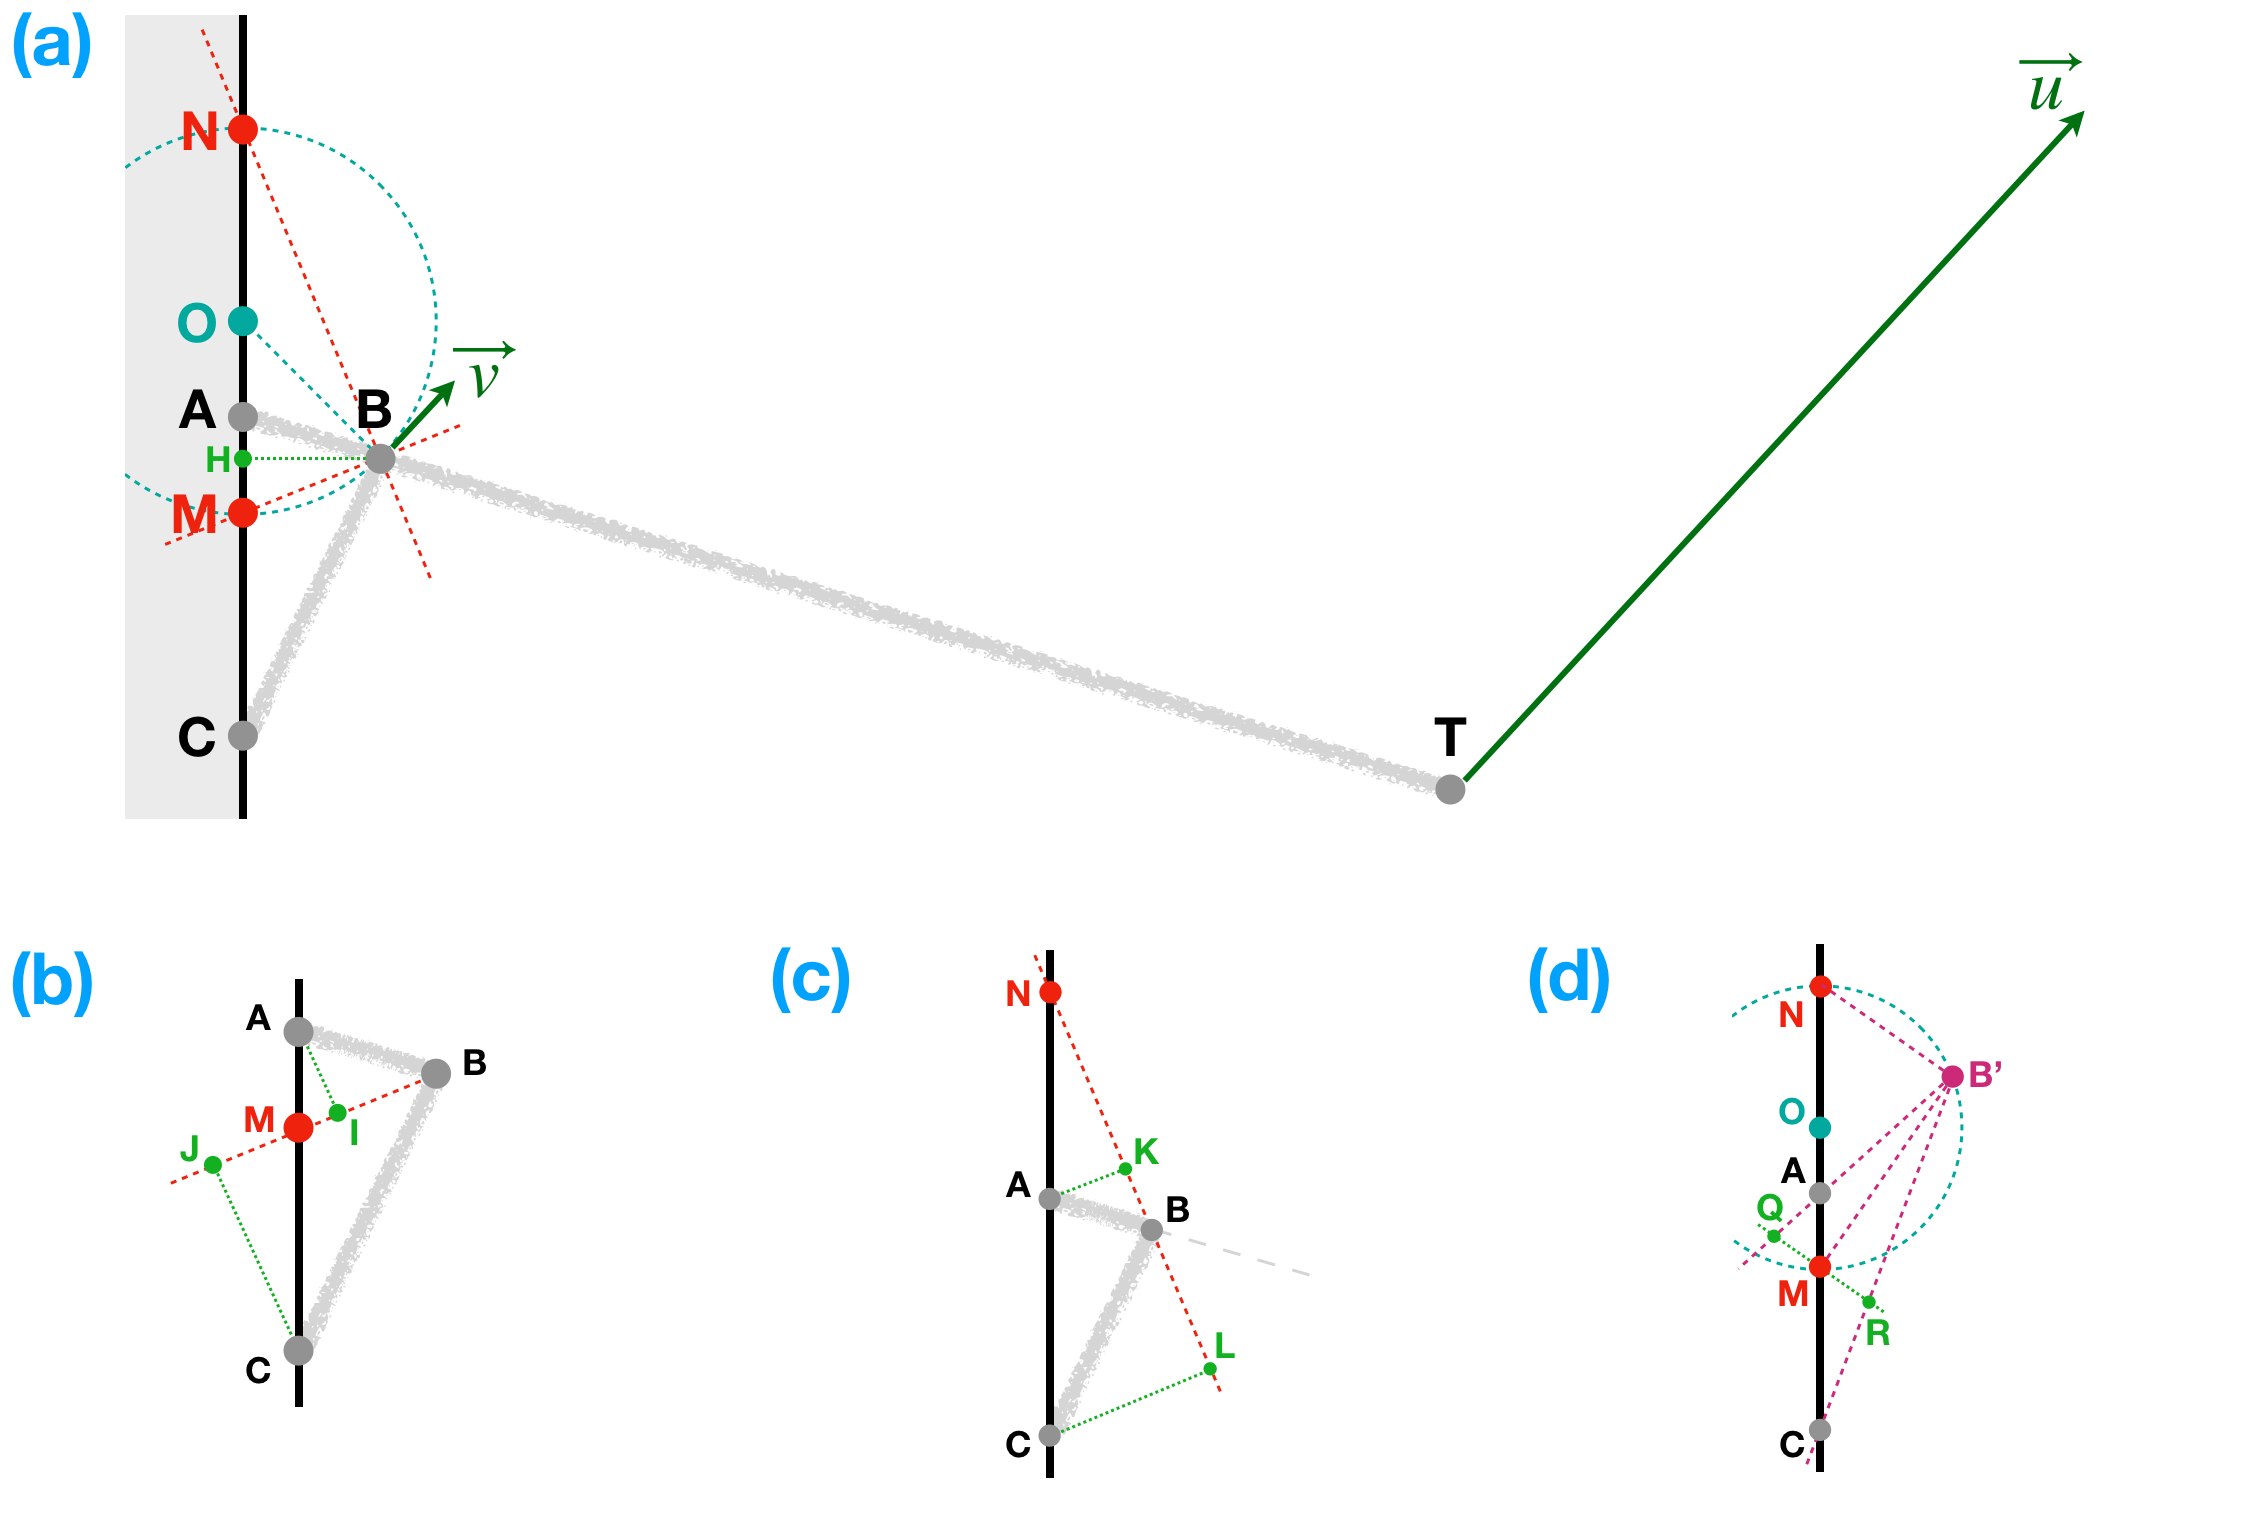
\includegraphics[width=\textwidth,keepaspectratio]{Problem_3/Figs/S3.png}
\end{center}

\ \

Kỳ thú và sảng khoái hơn nữa, với một điểm B' bất kỳ trên đường tròn tâm O đường kính MN thì ta luôn có B'M là phân giác góc $\widehat{\text{AB'C}}$. Chúng ta có thể chứng minh vắn như sau:

\begin{itemize}
     \item Từ M kẻ đường song song với B'N, cắt đường kéo dài B'A về phía A tại điểm Q và cắt đoạn B'C tại điểm R (xem hình minh họa \textbf{d}). Theo định lý Thalès, với MQ $\parallel$ B'N thì ta có $\overline{\text{MQ}}:\overline{\text{B'N}} = \overline{\text{AM}}:\overline{\text{AN}}$, với MR $\parallel$ B'N thì ta có $\overline{\text{MR}}:\overline{\text{B'N}} = \overline{\text{CM}}:\overline{\text{CN}}$. Sử dụng \eqref{distance}, thu được $\overline{\text{MQ}}=\overline{\text{QR}}$, tức M là trung điểm đoạn QR. Cùng với B'M vuông góc với QR, ta kết luận rằng tam giác $\Delta_\text{QB'R}$ cân ở B' và B'M là phân giác góc $\widehat{\text{QB'R}} \equiv \widehat{\text{AB'C}}$.
 \end{itemize}
    
\ \ 

Trong quá trình nở đều ra do nhiệt độ tăng lên (do thép là kim loại nở ra vì nhiệt), do tỉ số $\overline{\text{AB}}:\overline{\text{BC}}$ không đổi nên khớp B sẽ di chuyển trên đường tròn tâm O đường kính MN. Khoảng cách OB không đổi, tức véc-tơ vận tốc $\overrightarrow{v}$ của B sẽ vuông góc với đoạn OB. Như đã cho ở đề bài, thành phần vận tốc theo phương thẳng đứng của B là:
\begin{equation}
v_{\parallel} = \sin \widehat{\text{BOH}} .|\overrightarrow{v}| = \Big( \overline{\text{BH}}:\overline{\text{OB}}\Big) \vert \overrightarrow{v} \vert \ .
\label{v_veloc}
\end{equation}
Chiều cao $\overline{\text{BH}}$ có thể xác định được từ công thức Heron cho diện tích tam giác:
\begin{equation}
\begin{split}
\overline{\text{BH}} = \frac{2S(\Delta_{\text{ABC}})}{\overline{\text{AC}}} & = \frac{\sqrt{(s_1+s_2+s_3)(-s_1+s_2+s_3)(s_1-s_2+s_3)(s_1+s_2-s_3)}}{2s_3}
\\
& = \frac{\sqrt{(s_1^2+s_2^2+s_3^2)^2-2(s_1^4+s_2^4+s_3^4)}}{2s_3} \ .
\end{split}
\label{height}
\end{equation}
Chúng ta thế \eqref{radius} và \eqref{height} vào \eqref{v_veloc}, thu được giá trị độ lớn vận tốc của B:
\begin{equation}
\vert \overrightarrow{v} \vert = \frac{2s_1s_2 s_3^2}{(-s_1^2 + s_2^2)\sqrt{(s_1^2+s_2^2+s_3^2)^2-2(s_1^4+s_2^4+s_3^4)}} v_{\parallel} \ .
\label{v_mag}
\end{equation}
Thanh AT nở đều và quay quay khớp A ở vị trí cố định, nên do đồng dạng ta có liên hệ vận tốc:
 \begin{equation}
 \overrightarrow{u} = \left(\overline{\text{AT}} : \overline{\text{AB}} \right) . \overrightarrow{v} = \left( 1 + \frac{s_4}{s_1} \right) \overrightarrow{v} \ ,
 \end{equation}
 với $\overrightarrow{u}$ là vận tốc đầu thanh T. Thế nên, sử dụng \eqref{v_mag}:
\begin{equation}
\vert \overrightarrow{u} \vert = \frac{2s_1s_2 s_3^2 \left( 1 + \frac{s_4}{s_1}\right)}{(-s_1^2 + s_2^2)\sqrt{(s_1^2+s_2^2+s_3^2)^2-2(s_1^4+s_2^4+s_3^4)}} v_{\parallel} \ .
\label{u_mag}
\end{equation}
Vì $\overrightarrow{u} \parallel \overrightarrow{v}$ nên $\overrightarrow{u}$ cũng hợp với phương ngang góc $\theta = \widehat{\text{BOH}}$:
\begin{equation}
\begin{split}
 \theta &= \arcsin \Big( \overline{\text{BH}}:\overline{\text{OB}}\Big)
 \\
&= \arcsin \left[ \frac{(-s_1^2 + s_2^2)\sqrt{(s_1^2+s_2^2+s_3^2)^2-2(s_1^4+s_2^4+s_3^4)}}{2s_1s_2 s_3^2} \right] \ .
\end{split}
\label{angle}
\end{equation}

\ \ 

\textit{Dành cho các bạn muốn tìm hiểu sâu thêm, dễ dàng hơn để tổng quát với trường hợp hệ số nở về nhiệt của các thanh là khác nhau, nhưng cần phải phân tích vận tốc của khớp B ra thành phần quay và thành phần duỗi đối với từng thanh một. Phân tích này, thiết nghĩ, hơi vượt quá phạm vi kiến thức của học sinh THCS. Hy vọng sau khi đã vào cấp III, các bạn sẽ dành chút thời gian để tự giải lại bài tập theo hướng này.}

\newpage
{\normalcolor \textbf{CÂU 4 (4 điểm)}}\vspace{1.5mm}

\setcounter{equation}{0}
\textbf{Thấu kính tứ cực từ hội tụ mạnh}

Trong các máy gia tốc hạt năng lượng cao, việc điều hướng chuyển động của các hạt cần thông qua các tương tác điện từ. Tứ cực từ là một mô hình từ trường tạo ra bởi hệ thống dây điện được cuốn để sinh ra từ trường có dạng đường sức khá giống với bốn nam châm đặt đối xứng bốn góc và thường được sử dụng cho mục đích điều hướng chùm hạt. Trường điện từ của tứ cực từ sẽ tác dụng lực lên các hạt khiến cho quỹ đạo của chúng bị bẻ cong như cách các tia sáng đi qua các thấu kính quang học, nhưng lại chỉ bẻ hướng tia sáng về phía quang trục (như thấu kính hội tụ) theo một phương và bẻ hướng tia sáng ra xa khỏi quang trục (như thấu kính phân kỳ) theo phương còn lại. Trong bài toán này, chúng ta sẽ khảo sát định tính về mô hình tứ cực từ cũng như thiết kế một hệ các thấu kính tứ cực để tạo ra sự hội tụ cho chùm hạt.


\begin{enumerate}
    \item \textbf{Tính chất thú vị của tứ cực từ} \\
    Khi bạn lắp ráp bốn nam châm điện lại thành một hệ sao cho hai cực Nam ở đối diện nhau và hai cực Bắc ở đối diện nhau như hình \ref{fig:41}, bạn sẽ thu được một \textbf{tứ cực từ}. Tứ cực từ có rất nhiều tính chất thú vị, và được sử dụng rộng rãi trong các máy gia tốc hạt nhằm hội tụ các chùm tia tích điện. Các câu hỏi phía dưới sẽ khảo sát các đặc tính độc đáo của tứ cực từ:
    
    \begin{center}
    \begin{minipage}{0.45\textwidth}
    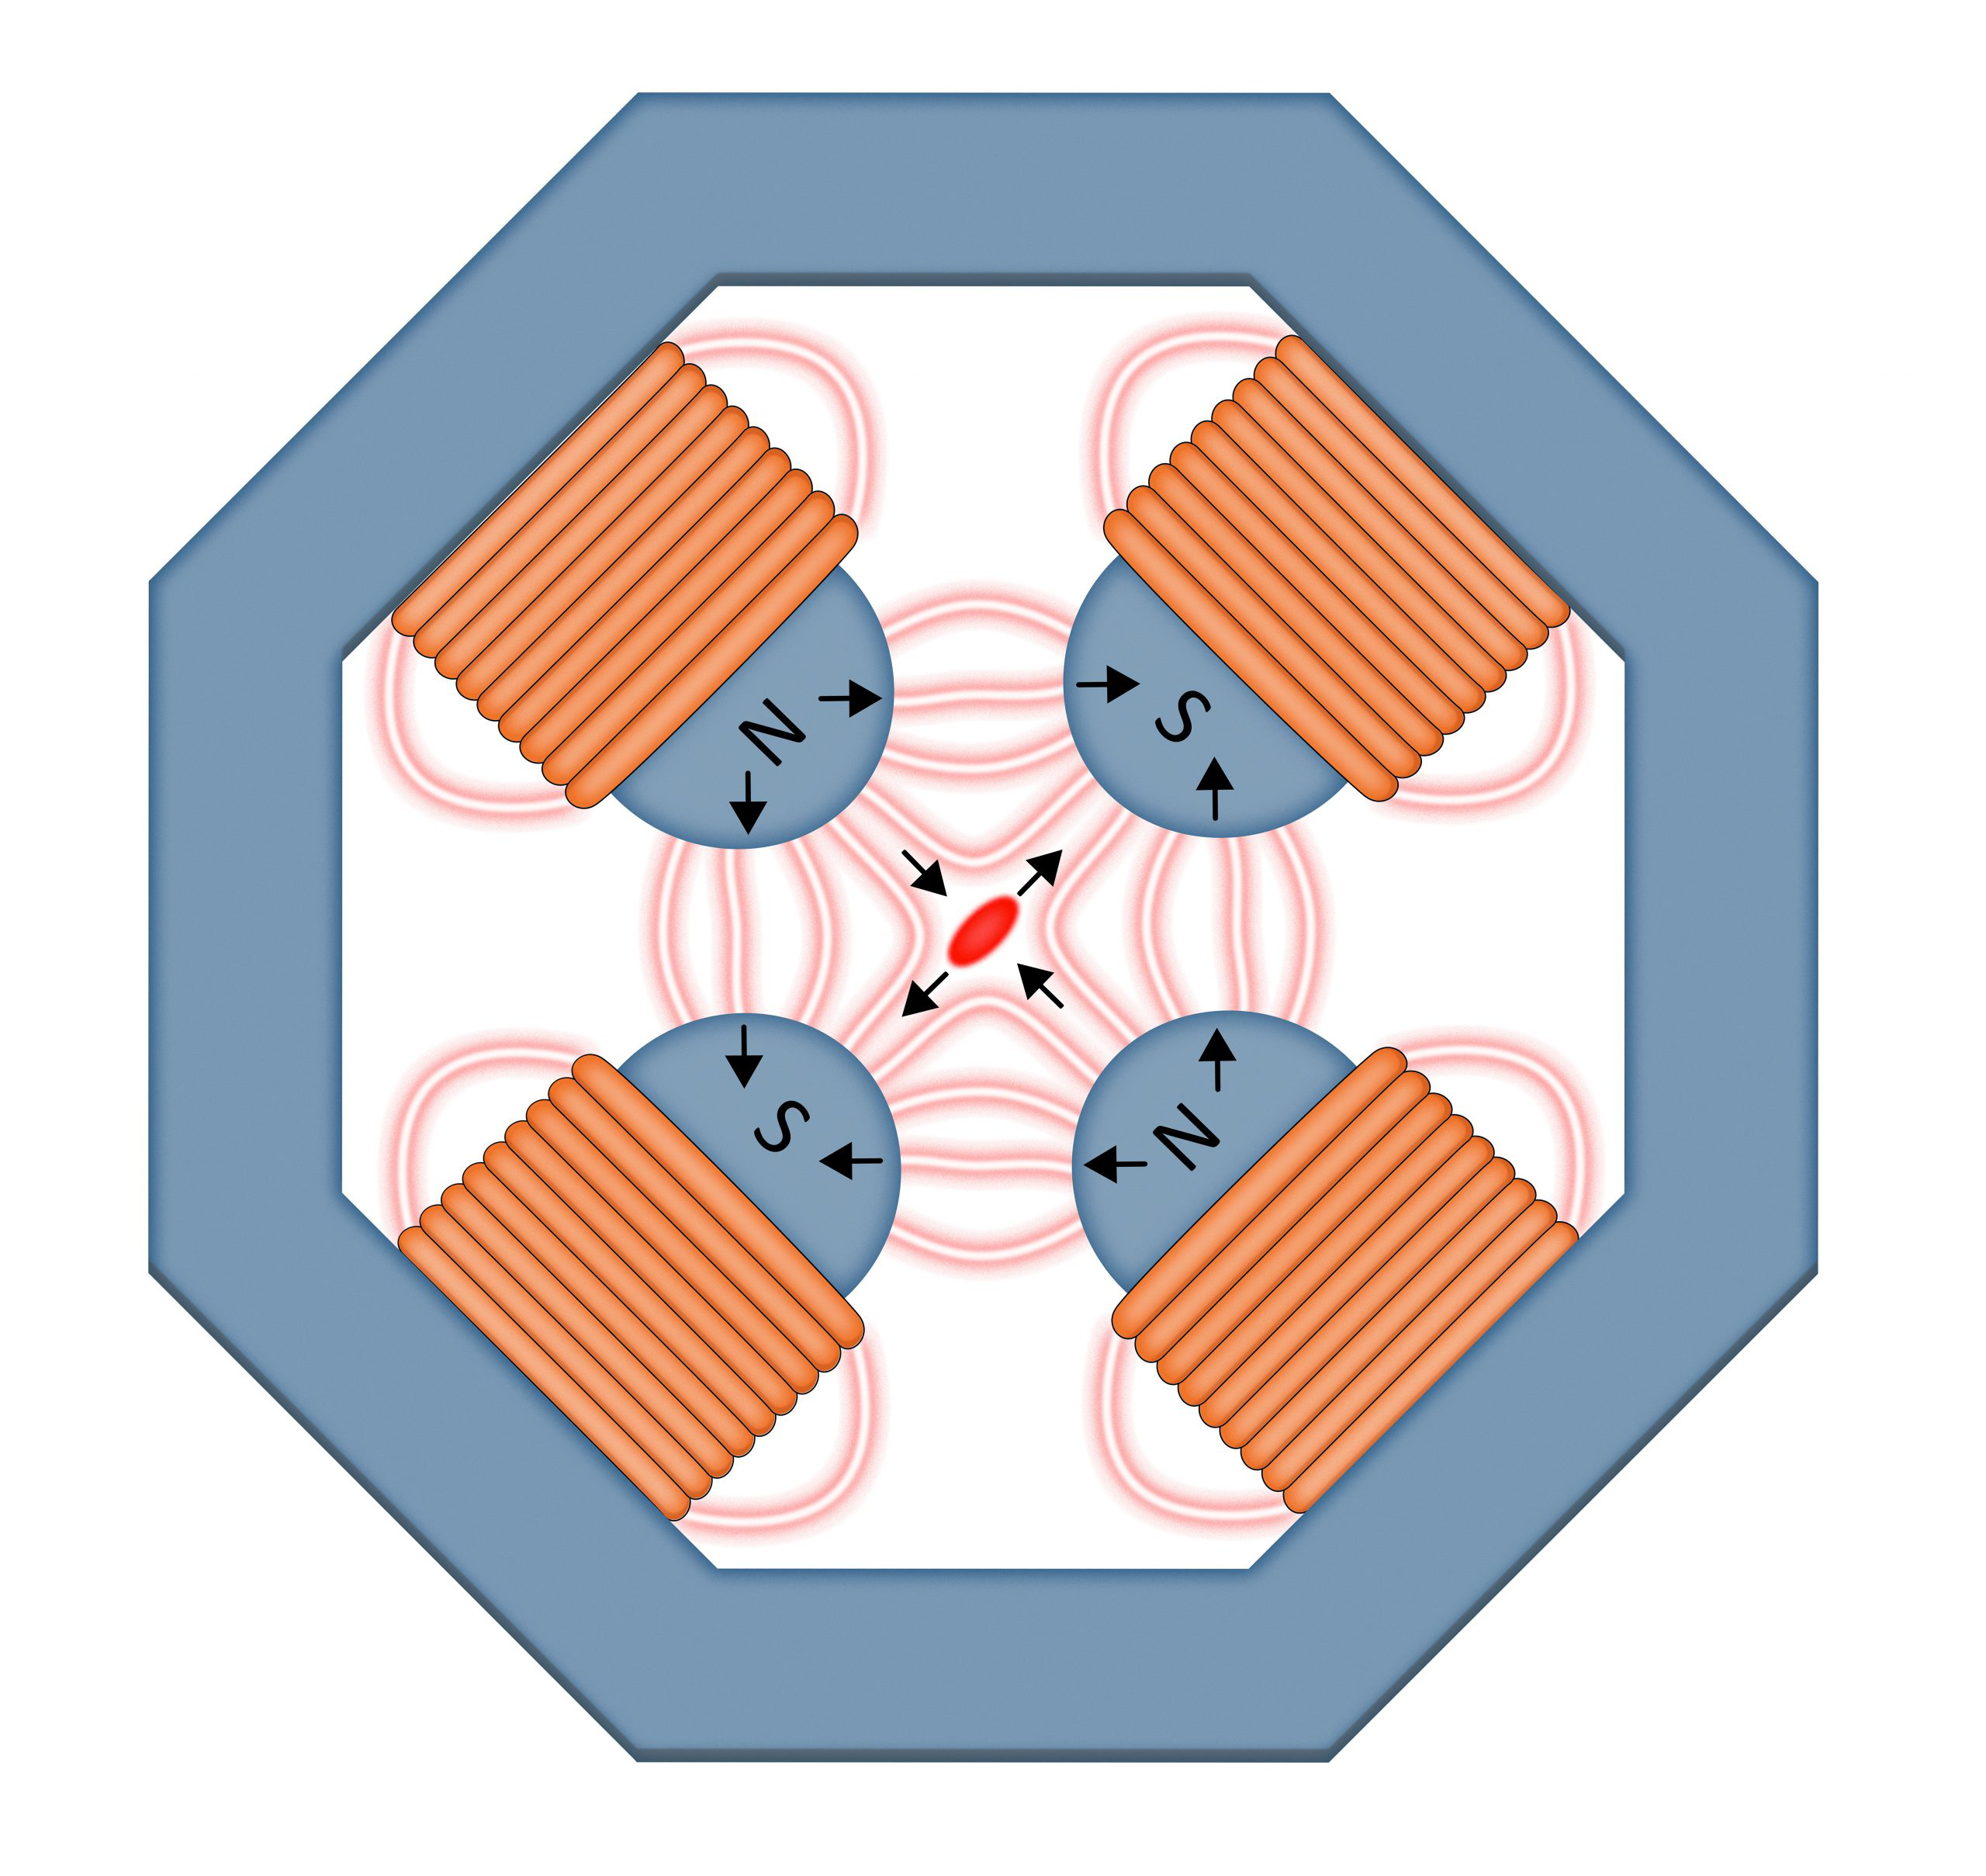
\includegraphics[width=0.9\textwidth]{Problem_4/quadrupoles.png}
    \end{minipage}
    \begin{minipage}{0.45\textwidth}
    \centering
    \scalebox{0.5}{
    \begin{tikzpicture}[x=0.75pt,y=0.75pt,yscale=-1,xscale=1]
        %uncomment if require: \path (0,642); %set diagram left start at 0, and has height of 642
        
        %Curve Lines [id:da4792522475831378] 
        \draw    (266,156) .. controls (356,227) and (358,227) .. (444,155) ;
        %Curve Lines [id:da18776678628173316] 
        \draw    (257,165) .. controls (365,254) and (349,254) .. (454,164) ;
        %Curve Lines [id:da7579049508332776] 
        \draw    (249,173) .. controls (367,283) and (346,283) .. (463,174) ;
        %Curve Lines [id:da9068961265681277] 
        \draw    (276,146) .. controls (354,204) and (363,204) .. (432,144) ;
        %Curve Lines [id:da6057096352515956] 
        \draw    (287,136) .. controls (356,191) and (359,191) .. (421,132) ;
        %Curve Lines [id:da6124834939512256] 
        \draw    (298,126) .. controls (346,161) and (367,161) .. (410,122) ;
        %Curve Lines [id:da999176140900975] 
        \draw    (309,115) .. controls (345,144) and (371,145) .. (403,114) ;
        %Curve Lines [id:da4412765595880592] 
        \draw    (315,108) .. controls (340,122) and (375,121) .. (397,108) ;
        %Curve Lines [id:da6165862171426286] 
        \draw    (327,97) .. controls (349,108) and (367,107) .. (386,97) ;
        %Curve Lines [id:da5352330674257251] 
        \draw    (337,86) .. controls (353,93) and (361,93) .. (373,85) ;
        %Straight Lines [id:da13696112022895202] 
        \draw    (241.18,179.89) -- (469.82,407.11) ;
        %Straight Lines [id:da612929119766775] 
        \draw    (239.67,405.57) -- (471.33,181.43) ;
        %Curve Lines [id:da9013347475427187] 
        \draw    (209.43,380.62) .. controls (281.45,292.07) and (284.48,289.13) .. (212.07,202.64) ;
        %Curve Lines [id:da8829915710419369] 
        \draw    (218.14,389.8) .. controls (308.32,283.62) and (308,299.62) .. (221.17,192.82) ;
        %Curve Lines [id:da839350917569065] 
        \draw    (225.88,397.96) .. controls (335.11,279.16) and (336.6,303.2) .. (231.24,184.02) ;
        %Curve Lines [id:da09708382750689237] 
        \draw    (199.74,370.42) .. controls (258.67,293.61) and (259.88,282.63) .. (200.95,214.41) ;
        %Curve Lines [id:da6233083389607426] 
        \draw    (190.08,359.22) .. controls (245.86,291.35) and (238.14,282.19) .. (188.87,225.17) ;
        %Curve Lines [id:da9303172125407404] 
        \draw    (180.42,348.02) .. controls (216,300.74) and (217.5,275.76) .. (178.76,235.96) ;
        %Curve Lines [id:da2769813795168756] 
        \draw    (169.77,336.8) .. controls (197.44,289.36) and (198.47,287.38) .. (170.71,242.8) ;
        %Curve Lines [id:da812357712173224] 
        \draw    (162.98,330.66) .. controls (176.4,302.93) and (177.05,270.94) .. (164.65,248.68) ;
        %Curve Lines [id:da730462575275286] 
        \draw    (152.35,318.44) .. controls (163.73,293.67) and (163.05,278.65) .. (153.55,259.45) ;
        %Curve Lines [id:da735579584390504] 
        \draw    (141.68,308.22) .. controls (148.93,292.37) and (147.11,284.33) .. (141.43,272.21) ;
        
        %Curve Lines [id:da9957314369504402] 
        \draw    (447.23,429.41) .. controls (356.24,360.51) and (353.19,357.59) .. (269.26,432.95) ;
        %Curve Lines [id:da42061516499279983] 
        \draw    (456.1,420.39) .. controls (346.85,333.94) and (362.85,333.72) .. (259.14,424.19) ;
        %Curve Lines [id:da6302289013179545] 
        \draw    (463.99,412.36) .. controls (341.47,307.32) and (365.44,305) .. (250,414.44) ;
        %Curve Lines [id:da6314722799353274] 
        \draw    (437.37,439.44) .. controls (358.56,383.22) and (347.55,382.39) .. (281.42,443.65) ;
        %Curve Lines [id:da7627601342878407] 
        \draw    (426.52,449.49) .. controls (356.74,396.1) and (347.86,404.14) .. (292.59,455.36) ;
        %Curve Lines [id:da5517437382717942] 
        \draw    (415.66,459.53) .. controls (367.17,425.61) and (342.16,424.98) .. (303.73,465.09) ;
        %Curve Lines [id:da2523109982366758] 
        \draw    (404.82,470.56) .. controls (356.44,444.56) and (354.42,443.6) .. (310.84,472.9) ;
        %Curve Lines [id:da5531448424788401] 
        \draw    (398.92,477.57) .. controls (370.73,465.12) and (338.74,465.57) .. (316.92,478.74) ;
        %Curve Lines [id:da8274878407169837] 
        \draw    (387.07,488.61) .. controls (361.92,478.1) and (346.93,479.3) .. (328.08,489.46) ;
        %Curve Lines [id:da2516778847803036] 
        \draw    (377.23,499.63) .. controls (361.13,492.94) and (353.16,495.03) .. (341.25,501.14) ;
        
        %Curve Lines [id:da44567985870338966] 
        \draw    (497.97,200.1) .. controls (426.63,289.2) and (423.63,292.16) .. (496.69,378.1) ;
        %Curve Lines [id:da18107514459279583] 
        \draw    (489.19,190.99) .. controls (399.82,297.86) and (400.03,281.86) .. (487.67,387.99) ;
        %Curve Lines [id:da3520275384011575] 
        \draw    (481.38,182.89) .. controls (373.06,302.52) and (371.39,278.5) .. (477.67,396.86) ;
        %Curve Lines [id:da5409134618202889] 
        \draw    (507.73,210.23) .. controls (449.39,287.49) and (448.27,298.48) .. (507.72,366.24) ;
        %Curve Lines [id:da5658457580650191] 
        \draw    (517.48,221.35) .. controls (462.22,289.65) and (470.02,298.75) .. (519.72,355.39) ;
        %Curve Lines [id:da41437201980134053] 
        \draw    (527.22,232.48) .. controls (492.01,280.03) and (490.7,305.02) .. (529.75,344.52) ;
        %Curve Lines [id:da607470080861005] 
        \draw    (537.96,243.62) .. controls (510.65,291.27) and (509.64,293.26) .. (537.75,337.62) ;
        %Curve Lines [id:da3226182027720166] 
        \draw    (544.8,249.7) .. controls (531.59,277.54) and (531.18,309.53) .. (543.76,331.7) ;
        %Curve Lines [id:da59845594322587] 
        \draw    (555.52,261.84) .. controls (544.33,286.7) and (545.13,301.71) .. (554.77,320.84) ;
        %Curve Lines [id:da3781492316292461] 
        \draw    (566.27,271.98) .. controls (559.15,287.89) and (561.02,295.91) .. (566.8,307.99) ;
        
        %Straight Lines [id:da8548346448041899] 
        \draw    (76,556) -- (74.01,44) ;
        \draw [shift={(74,42)}, rotate = 89.78] [color={rgb, 255:red, 0; green, 0; blue, 0 }  ][line width=0.75]    (10.93,-3.29) .. controls (6.95,-1.4) and (3.31,-0.3) .. (0,0) .. controls (3.31,0.3) and (6.95,1.4) .. (10.93,3.29)   ;
        %Straight Lines [id:da8984436400560898] 
        \draw    (76,556) -- (626,555) ;
        \draw [shift={(628,555)}, rotate = 179.9] [color={rgb, 255:red, 0; green, 0; blue, 0 }  ][line width=0.75]    (10.93,-3.29) .. controls (6.95,-1.4) and (3.31,-0.3) .. (0,0) .. controls (3.31,0.3) and (6.95,1.4) .. (10.93,3.29)   ;
        \draw   (349,222) -- (364,231) -- (349,240) ;
        \draw   (295.58,280.6) -- (286.41,295.5) -- (277.59,280.4) ;
        \draw   (365.2,365.83) -- (350,357.16) -- (364.8,347.84) ;
        \draw   (414.6,297.62) -- (423.4,282.5) -- (432.6,297.38) ;
        
        % Text Node
        \draw (183,119.4) node [anchor=north west][inner sep=0.75pt]  [font=\Huge,color={rgb, 255:red, 208; green, 2; blue, 27 }  ,opacity=1 ]  {$N$};
        % Text Node
        \draw (490,407.4) node [anchor=north west][inner sep=0.75pt]  [font=\Huge,color={rgb, 255:red, 208; green, 2; blue, 27 }  ,opacity=1 ]  {$N$};
        % Text Node
        \draw (503,120.4) node [anchor=north west][inner sep=0.75pt]  [font=\Huge,color={rgb, 255:red, 65; green, 117; blue, 5 }  ,opacity=1 ]  {$S$};
        % Text Node
        \draw (190,410.4) node [anchor=north west][inner sep=0.75pt]  [font=\Huge,color={rgb, 255:red, 65; green, 117; blue, 5 }  ,opacity=1 ]  {$S$};
        % Text Node
        \draw (42,559.4) node [anchor=north west][inner sep=0.75pt]  [font=\huge]  {$O$};
        % Text Node
        \draw (603,563) node [anchor=north west][inner sep=0.75pt]  [font=\huge]  {$x$};
        % Text Node
        \draw (42,34.4) node [anchor=north west][inner sep=0.75pt]  [font=\huge]  {$y$};


    \end{tikzpicture}
    }
    \end{minipage} \\
    %\caption{Mô hình tứ cực từ trong thực tế (bên trái) và từ phổ của tứ cực từ (bên phải)}
    \captionof{figure}{Mô hình tứ cực từ trong thực tế (bên trái) và từ phổ của tứ cực từ (bên phải)}
    \label{fig:41}
    \end{center}
    
    Cho từ phổ của một tứ cực từ. Dựa vào hình \ref{fig:41}, hãy xác định phương, chiều của \textbf{đường sức từ} và \textbf{lực điện từ} tác dụng lên một hạt điện tích nhỏ bay vào tứ cực từ với phương vuông góc với trang giấy, chiều ra xa người đọc. 

    \item \textbf{Ứng dụng trong việc hội tụ chùm tia} \\
    Sau khi đã xác định được lực điện từ tác dụng lên hạt điện tích, ta có thể thấy rằng theo phương $y$, hạt sẽ bị đẩy vào bên trong tứ cực từ, còn theo phương $x$, hạt sẽ bị đẩy ra xa tứ cực từ. Hay nói cách khác, nếu ta coi tứ cực từ là một thấu kính thì thấu kính này sẽ \textbf{hội tụ} trên phương $y$ và \textbf{phân kì} trên phương $x$ với cùng một tiêu cự $f$. Nếu ta lật ngược thấu kính đi $90^\circ$ thì thấu kính sẽ phân kỳ trên phương $y$ và hội tụ trên phương $x$.
    
    \begin{figure}[!ht]
    \centering
    \scalebox{0.9}{
    \begin{tikzpicture}[x=0.75pt,y=0.75pt,yscale=-1,xscale=1]
        %uncomment if require: \path (0,424); %set diagram left start at 0, and has height of 424
        
        %Straight Lines [id:da6678677431158608] 
        \draw    (51,378) -- (181,378) ;
        %Straight Lines [id:da673747824550079] 
        \draw    (51,259) -- (181,259) ;
        %Straight Lines [id:da3567165573223894] 
        \draw    (51,259) -- (51,378) ;
        %Straight Lines [id:da4131289268440297] 
        \draw    (181,259) -- (181,378) ;
        %Curve Lines [id:da6284585681017343] 
        \draw    (51,289) .. controls (82,288) and (82,284) .. (83,259) ;
        %Curve Lines [id:da7073873859904605] 
        \draw    (51,346) .. controls (83,348) and (83,348) .. (83,378) ;
        %Curve Lines [id:da3036947661512792] 
        \draw    (149,259) .. controls (150,291) and (150,291) .. (181,291) ;
        %Curve Lines [id:da9150242892043405] 
        \draw    (151,378) .. controls (151,346) and (151,346) .. (182,346) ;
        
        %Straight Lines [id:da8908202829099343] 
        \draw    (245,271) -- (375,271) ;
        %Straight Lines [id:da2173944797906926] 
        \draw    (245,152) -- (375,152) ;
        %Straight Lines [id:da3230976467548934] 
        \draw    (245,152) -- (245,271) ;
        %Straight Lines [id:da37549197915656185] 
        \draw    (375,152) -- (375,271) ;
        %Curve Lines [id:da11844780145514733] 
        \draw    (245,182) .. controls (276,181) and (276,177) .. (277,152) ;
        %Curve Lines [id:da19840673204511416] 
        \draw    (245,239) .. controls (277,241) and (277,241) .. (277,271) ;
        %Curve Lines [id:da07608929271157883] 
        \draw    (343,152) .. controls (344,184) and (344,184) .. (375,184) ;
        %Curve Lines [id:da590005125259021] 
        \draw    (345,271) .. controls (345,239) and (345,239) .. (376,239) ;
        %Straight Lines [id:da8314279294962961] 
        \draw  [dash pattern={on 0.84pt off 2.51pt}]  (181,378) -- (573,162) ;
        %Straight Lines [id:da09601563855642858] 
        \draw    (115,320) -- (205,320) ;
        \draw [shift={(207,320)}, rotate = 180] [color={rgb, 255:red, 0; green, 0; blue, 0 }  ][line width=0.75]    (10.93,-3.29) .. controls (6.95,-1.4) and (3.31,-0.3) .. (0,0) .. controls (3.31,0.3) and (6.95,1.4) .. (10.93,3.29)   ;
        %Straight Lines [id:da8517185652543424] 
        \draw    (115,320) -- (115,228) ;
        \draw [shift={(115,226)}, rotate = 90] [color={rgb, 255:red, 0; green, 0; blue, 0 }  ][line width=0.75]    (10.93,-3.29) .. controls (6.95,-1.4) and (3.31,-0.3) .. (0,0) .. controls (3.31,0.3) and (6.95,1.4) .. (10.93,3.29)   ;
        %Straight Lines [id:da9476216664675472] 
        \draw  [dash pattern={on 4.5pt off 4.5pt}]  (443,162) -- (573,162) ;
        %Straight Lines [id:da7668565905633495] 
        \draw  [dash pattern={on 4.5pt off 4.5pt}]  (443,43) -- (573,43) ;
        %Straight Lines [id:da6517531350813479] 
        \draw  [dash pattern={on 4.5pt off 4.5pt}]  (443,43) -- (443,162) ;
        %Straight Lines [id:da05757003100942071] 
        \draw  [dash pattern={on 4.5pt off 4.5pt}]  (573,43) -- (573,162) ;
        %Straight Lines [id:da1731975813788058] 
        \draw  [dash pattern={on 4.5pt off 4.5pt}]  (38,363) -- (600.25,51.97) ;
        \draw [shift={(602,51)}, rotate = 151.05] [color={rgb, 255:red, 0; green, 0; blue, 0 }  ][line width=0.75]    (10.93,-3.29) .. controls (6.95,-1.4) and (3.31,-0.3) .. (0,0) .. controls (3.31,0.3) and (6.95,1.4) .. (10.93,3.29)   ;
        %Shape: Circle [id:dp49351180655100846] 
        \draw  [fill={rgb, 255:red, 74; green, 144; blue, 226 }  ,fill opacity=1 ] (127,288.5) .. controls (127,287.12) and (128.12,286) .. (129.5,286) .. controls (130.88,286) and (132,287.12) .. (132,288.5) .. controls (132,289.88) and (130.88,291) .. (129.5,291) .. controls (128.12,291) and (127,289.88) .. (127,288.5) -- cycle ;
        %Shape: Circle [id:dp062066057993846346] 
        \draw  [fill={rgb, 255:red, 74; green, 144; blue, 226 }  ,fill opacity=1 ] (291,176.5) .. controls (291,175.12) and (292.12,174) .. (293.5,174) .. controls (294.88,174) and (296,175.12) .. (296,176.5) .. controls (296,177.88) and (294.88,179) .. (293.5,179) .. controls (292.12,179) and (291,177.88) .. (291,176.5) -- cycle ;
        %Straight Lines [id:da517606792137199] 
        \draw    (151,236) -- (130.26,286.65) ;
        \draw [shift={(129.5,288.5)}, rotate = 292.27] [color={rgb, 255:red, 0; green, 0; blue, 0 }  ][line width=0.75]    (10.93,-3.29) .. controls (6.95,-1.4) and (3.31,-0.3) .. (0,0) .. controls (3.31,0.3) and (6.95,1.4) .. (10.93,3.29)   ;
        %Straight Lines [id:da9135691624456295] 
        \draw    (315,124) -- (294.26,174.65) ;
        \draw [shift={(293.5,176.5)}, rotate = 292.27] [color={rgb, 255:red, 0; green, 0; blue, 0 }  ][line width=0.75]    (10.93,-3.29) .. controls (6.95,-1.4) and (3.31,-0.3) .. (0,0) .. controls (3.31,0.3) and (6.95,1.4) .. (10.93,3.29)   ;
        %Shape: Circle [id:dp13300062616731956] 
        \draw  [fill={rgb, 255:red, 74; green, 144; blue, 226 }  ,fill opacity=1 ] (504,104.5) .. controls (504,103.12) and (505.12,102) .. (506.5,102) .. controls (507.88,102) and (509,103.12) .. (509,104.5) .. controls (509,105.88) and (507.88,107) .. (506.5,107) .. controls (505.12,107) and (504,105.88) .. (504,104.5) -- cycle ;
        
        % Text Node
        \draw (57,266.4) node [anchor=north west][inner sep=0.75pt]  [color={rgb, 255:red, 208; green, 2; blue, 27 }  ,opacity=1 ]  {$N$};
        % Text Node
        \draw (158,355.4) node [anchor=north west][inner sep=0.75pt]  [color={rgb, 255:red, 208; green, 2; blue, 27 }  ,opacity=1 ]  {$N$};
        % Text Node
        \draw (160,265.4) node [anchor=north west][inner sep=0.75pt]  [color={rgb, 255:red, 208; green, 2; blue, 27 }  ,opacity=1 ]  {$\textcolor[rgb]{0.25,0.46,0.02}{S}$};
        % Text Node
        \draw (60,355.4) node [anchor=north west][inner sep=0.75pt]  [color={rgb, 255:red, 208; green, 2; blue, 27 }  ,opacity=1 ]  {$\textcolor[rgb]{0.25,0.46,0.02}{S}$};
        % Text Node
        \draw (251,248.4) node [anchor=north west][inner sep=0.75pt]  [color={rgb, 255:red, 208; green, 2; blue, 27 }  ,opacity=1 ]  {$N$};
        % Text Node
        \draw (353,157.4) node [anchor=north west][inner sep=0.75pt]  [color={rgb, 255:red, 208; green, 2; blue, 27 }  ,opacity=1 ]  {$N$};
        % Text Node
        \draw (252,157.4) node [anchor=north west][inner sep=0.75pt]  [color={rgb, 255:red, 208; green, 2; blue, 27 }  ,opacity=1 ]  {$\textcolor[rgb]{0.25,0.46,0.02}{S}$};
        % Text Node
        \draw (355,249.4) node [anchor=north west][inner sep=0.75pt]  [color={rgb, 255:red, 208; green, 2; blue, 27 }  ,opacity=1 ]  {$\textcolor[rgb]{0.25,0.46,0.02}{S}$};
        % Text Node
        \draw (204,297.4) node [anchor=north west][inner sep=0.75pt]    {$x$};
        % Text Node
        \draw (97,218.4) node [anchor=north west][inner sep=0.75pt]    {$y$};
        % Text Node
        \draw (94,298.4) node [anchor=north west][inner sep=0.75pt]    {$O$};
        % Text Node
        \draw (607,38.4) node [anchor=north west][inner sep=0.75pt]    {$z$};
        % Text Node
        \draw (141,211.4) node [anchor=north west][inner sep=0.75pt]    {$A( x_{0} ,y_{0})$};
        % Text Node
        \draw (300,100.4) node [anchor=north west][inner sep=0.75pt]    {$B( x,y)$};
        % Text Node
        \draw (464.5,80.4) node [anchor=north west][inner sep=0.75pt]    {$C( 0,0)$};
        % Text Node
        \draw (286,324.4) node [anchor=north west][inner sep=0.75pt]    {$L$};
        % Text Node
        \draw (466,228.4) node [anchor=north west][inner sep=0.75pt]    {$L$};
        % Text Node
        \draw (23,221.4) node [anchor=north west][inner sep=0.75pt]  [font=\Large]  {$Q_{1}$};
        % Text Node
        \draw (216,116.4) node [anchor=north west][inner sep=0.75pt]  [font=\Large]  {$Q_{2}$};


    \end{tikzpicture}
    } \\
    \caption{Hệ hai thấu kính tứ cực từ}
    \label{fig:42}
    \end{figure}

     Vì tính chất độc đáo này, các nhà khoa học thường dùng các hệ thấu kính tứ cực từ để hội tụ các chùm hạt tích điện trong máy gia tốc hạt. Xét một hệ hai thấu kính tứ cực từ $Q_1$ và $Q_2$ như hình \ref{fig:42}. Các thấu kính cách nhau một đoạn $L$ theo phương $z$, và thấu kính $Q_1$ có tiêu cự trên cả hai phương $x$ và $y$ đều là $f_x = f_y = f$. Ban đầu, có một hạt nhỏ bắn dọc theo phương $z$ vào $Q_1$ tại vị trí $A(x_0, y_0)$. 

    \begin{enumerate}
        \item 
        Xác định tọa độ $B(x,y)$ của hạt khi hạt đến thấu kính $Q_2$ (giả sử các thấu kính đủ rộng để hạt không bị bắn ra ngoài thấu kính).
        \item 
        Tìm điều kiện của $f$ để khi tới điểm cách thấu kính $Q_2$ đoạn $L$, hạt sẽ hội tụ tại điểm $C(0,0)$. Tính tiêu cự $f$ của thấu kính $Q_1$ và $f'$ của thấu kính $Q_2$.
    \end{enumerate}
\end{enumerate}

\begin{flushright}
   \normalcolor(Biên soạn bởi Colevol)
\end{flushright}
\setcounter{equation}{0}
\begin{center}
    \normalcolor{\textbf{Bài giải}}
\end{center}
\begin{enumerate}
    \item
    Từ hình \ref{fig:41}, ta có thể dễ dàng chỉ ra được phương và chiều của đường sức từ như hình \ref{fig:43}. \\

    Áp dụng quy tắc bàn tay trái: Đặt bàn tay sao cho ngón tró chỉ vào màn hình, lòng bàn tay hướng sao để nhận được các đường sức từ vuông góc với mặt bàn tay. Ngón cái duỗi thẳng ra sẽ là chiều của lực điện từ, được mô tả như hình \ref{fig:43}. \\

    \textbf{Bình luận}: Bằng các kiến thức về trường điện từ, động lực học và động lực học tương đối tính, ta có thể  để giải thích về quỹ đạo của hạt khi đi vào tứ cực từ. Cụ thể, trên phương $y$, do lực điện từ luôn hướng vào tâm của tứ cực từ nên hạt sẽ bị \textbf{hội tụ}. Tương tự, trên phương $x$, lực điện từ đều hướng ra xa tâm của tứ cực từ nên hạt sẽ bị \textbf{phân kì}. 
    
    \begin{figure}[!ht]
    \centering
    \scalebox{0.82}{
    \begin{tikzpicture}[x=0.75pt,y=0.75pt,yscale=-1,xscale=1]
        %uncomment if require: \path (0,642); %set diagram left start at 0, and has height of 642
        
        %Curve Lines [id:da4792522475831378] 
        \draw    (266,156) .. controls (356,227) and (358,227) .. (444,155) ;
        %Curve Lines [id:da18776678628173316] 
        \draw    (257,165) .. controls (365,254) and (349,254) .. (454,164) ;
        %Curve Lines [id:da7579049508332776] 
        \draw    (249,173) .. controls (367,283) and (346,283) .. (463,174) ;
        %Curve Lines [id:da9068961265681277] 
        \draw    (276,146) .. controls (354,204) and (363,204) .. (432,144) ;
        %Curve Lines [id:da6057096352515956] 
        \draw    (287,136) .. controls (356,191) and (359,191) .. (421,132) ;
        %Curve Lines [id:da6124834939512256] 
        \draw    (298,126) .. controls (346,161) and (367,161) .. (410,122) ;
        %Curve Lines [id:da999176140900975] 
        \draw    (309,115) .. controls (345,144) and (371,145) .. (403,114) ;
        %Curve Lines [id:da4412765595880592] 
        \draw    (315,108) .. controls (340,122) and (375,121) .. (397,108) ;
        %Curve Lines [id:da6165862171426286] 
        \draw    (327,97) .. controls (349,108) and (367,107) .. (386,97) ;
        %Curve Lines [id:da5352330674257251] 
        \draw    (337,86) .. controls (353,93) and (361,93) .. (373,85) ;
        %Straight Lines [id:da13696112022895202] 
        \draw    (241.18,179.89) -- (469.82,407.11) ;
        %Straight Lines [id:da612929119766775] 
        \draw    (239.67,405.57) -- (471.33,181.43) ;
        %Curve Lines [id:da9013347475427187] 
        \draw    (209.43,380.62) .. controls (281.45,292.07) and (284.48,289.13) .. (212.07,202.64) ;
        %Curve Lines [id:da8829915710419369] 
        \draw    (218.14,389.8) .. controls (308.32,283.62) and (308,299.62) .. (221.17,192.82) ;
        %Curve Lines [id:da839350917569065] 
        \draw    (225.88,397.96) .. controls (335.11,279.16) and (336.6,303.2) .. (231.24,184.02) ;
        %Curve Lines [id:da09708382750689237] 
        \draw    (199.74,370.42) .. controls (258.67,293.61) and (259.88,282.63) .. (200.95,214.41) ;
        %Curve Lines [id:da6233083389607426] 
        \draw    (190.08,359.22) .. controls (245.86,291.35) and (238.14,282.19) .. (188.87,225.17) ;
        %Curve Lines [id:da9303172125407404] 
        \draw    (180.42,348.02) .. controls (216,300.74) and (217.5,275.76) .. (178.76,235.96) ;
        %Curve Lines [id:da2769813795168756] 
        \draw    (169.77,336.8) .. controls (197.44,289.36) and (198.47,287.38) .. (170.71,242.8) ;
        %Curve Lines [id:da812357712173224] 
        \draw    (162.98,330.66) .. controls (176.4,302.93) and (177.05,270.94) .. (164.65,248.68) ;
        %Curve Lines [id:da730462575275286] 
        \draw    (152.35,318.44) .. controls (163.73,293.67) and (163.05,278.65) .. (153.55,259.45) ;
        %Curve Lines [id:da735579584390504] 
        \draw    (141.68,308.22) .. controls (148.93,292.37) and (147.11,284.33) .. (141.43,272.21) ;
        
        %Curve Lines [id:da9957314369504402] 
        \draw    (447.23,429.41) .. controls (356.24,360.51) and (353.19,357.59) .. (269.26,432.95) ;
        %Curve Lines [id:da42061516499279983] 
        \draw    (456.1,420.39) .. controls (346.85,333.94) and (362.85,333.72) .. (259.14,424.19) ;
        %Curve Lines [id:da6302289013179545] 
        \draw    (463.99,412.36) .. controls (341.47,307.32) and (365.44,305) .. (250,414.44) ;
        %Curve Lines [id:da6314722799353274] 
        \draw    (437.37,439.44) .. controls (358.56,383.22) and (347.55,382.39) .. (281.42,443.65) ;
        %Curve Lines [id:da7627601342878407] 
        \draw    (426.52,449.49) .. controls (356.74,396.1) and (347.86,404.14) .. (292.59,455.36) ;
        %Curve Lines [id:da5517437382717942] 
        \draw    (415.66,459.53) .. controls (367.17,425.61) and (342.16,424.98) .. (303.73,465.09) ;
        %Curve Lines [id:da2523109982366758] 
        \draw    (404.82,470.56) .. controls (356.44,444.56) and (354.42,443.6) .. (310.84,472.9) ;
        %Curve Lines [id:da5531448424788401] 
        \draw    (398.92,477.57) .. controls (370.73,465.12) and (338.74,465.57) .. (316.92,478.74) ;
        %Curve Lines [id:da8274878407169837] 
        \draw    (387.07,488.61) .. controls (361.92,478.1) and (346.93,479.3) .. (328.08,489.46) ;
        %Curve Lines [id:da2516778847803036] 
        \draw    (377.23,499.63) .. controls (361.13,492.94) and (353.16,495.03) .. (341.25,501.14) ;
        
        %Curve Lines [id:da44567985870338966] 
        \draw    (497.97,200.1) .. controls (426.63,289.2) and (423.63,292.16) .. (496.69,378.1) ;
        %Curve Lines [id:da18107514459279583] 
        \draw    (489.19,190.99) .. controls (399.82,297.86) and (400.03,281.86) .. (487.67,387.99) ;
        %Curve Lines [id:da3520275384011575] 
        \draw    (481.38,182.89) .. controls (373.06,302.52) and (371.39,278.5) .. (477.67,396.86) ;
        %Curve Lines [id:da5409134618202889] 
        \draw    (507.73,210.23) .. controls (449.39,287.49) and (448.27,298.48) .. (507.72,366.24) ;
        %Curve Lines [id:da5658457580650191] 
        \draw    (517.48,221.35) .. controls (462.22,289.65) and (470.02,298.75) .. (519.72,355.39) ;
        %Curve Lines [id:da41437201980134053] 
        \draw    (527.22,232.48) .. controls (492.01,280.03) and (490.7,305.02) .. (529.75,344.52) ;
        %Curve Lines [id:da607470080861005] 
        \draw    (537.96,243.62) .. controls (510.65,291.27) and (509.64,293.26) .. (537.75,337.62) ;
        %Curve Lines [id:da3226182027720166] 
        \draw    (544.8,249.7) .. controls (531.59,277.54) and (531.18,309.53) .. (543.76,331.7) ;
        %Curve Lines [id:da59845594322587] 
        \draw    (555.52,261.84) .. controls (544.33,286.7) and (545.13,301.71) .. (554.77,320.84) ;
        %Curve Lines [id:da3781492316292461] 
        \draw    (566.27,271.98) .. controls (559.15,287.89) and (561.02,295.91) .. (566.8,307.99) ;
        
        %Straight Lines [id:da8548346448041899] 
        \draw    (76,556) -- (74.01,44) ;
        \draw [shift={(74,42)}, rotate = 89.78] [color={rgb, 255:red, 0; green, 0; blue, 0 }  ][line width=0.75]    (10.93,-3.29) .. controls (6.95,-1.4) and (3.31,-0.3) .. (0,0) .. controls (3.31,0.3) and (6.95,1.4) .. (10.93,3.29)   ;
        %Straight Lines [id:da8984436400560898] 
        \draw    (76,556) -- (626,555) ;
        \draw [shift={(628,555)}, rotate = 179.9] [color={rgb, 255:red, 0; green, 0; blue, 0 }  ][line width=0.75]    (10.93,-3.29) .. controls (6.95,-1.4) and (3.31,-0.3) .. (0,0) .. controls (3.31,0.3) and (6.95,1.4) .. (10.93,3.29)   ;
        \draw   (349,222) -- (364,231) -- (349,240) ;
        \draw   (295.58,280.6) -- (286.41,295.5) -- (277.59,280.4) ;
        \draw   (365.2,365.83) -- (350,357.16) -- (364.8,347.84) ;
        \draw   (414.6,297.62) -- (423.4,282.5) -- (432.6,297.38) ;
        %Straight Lines [id:da6158567950762239] 
        \draw [color={rgb, 255:red, 231; green, 16; blue, 41 }  ,draw opacity=1 ][line width=2.25]    (357,209) -- (430,209) ;
        \draw [shift={(434,209)}, rotate = 180] [color={rgb, 255:red, 231; green, 16; blue, 41 }  ,draw opacity=1 ][line width=2.25]    (17.49,-5.26) .. controls (11.12,-2.23) and (5.29,-0.48) .. (0,0) .. controls (5.29,0.48) and (11.12,2.23) .. (17.49,5.26)   ;
        %Straight Lines [id:da4424105608351112] 
        \draw [color={rgb, 255:red, 231; green, 16; blue, 41 }  ,draw opacity=1 ][line width=2.25]    (265,288) -- (265,349) ;
        \draw [shift={(265,353)}, rotate = 270] [color={rgb, 255:red, 231; green, 16; blue, 41 }  ,draw opacity=1 ][line width=2.25]    (17.49,-5.26) .. controls (11.12,-2.23) and (5.29,-0.48) .. (0,0) .. controls (5.29,0.48) and (11.12,2.23) .. (17.49,5.26)   ;
        %Straight Lines [id:da6470847365790864] 
        \draw [color={rgb, 255:red, 231; green, 16; blue, 41 }  ,draw opacity=1 ][line width=2.25]    (358,376) -- (295,376) ;
        \draw [shift={(291,376)}, rotate = 360] [color={rgb, 255:red, 231; green, 16; blue, 41 }  ,draw opacity=1 ][line width=2.25]    (17.49,-5.26) .. controls (11.12,-2.23) and (5.29,-0.48) .. (0,0) .. controls (5.29,0.48) and (11.12,2.23) .. (17.49,5.26)   ;
        %Straight Lines [id:da3950467179843975] 
        \draw [color={rgb, 255:red, 231; green, 16; blue, 41 }  ,draw opacity=1 ][line width=2.25]    (443,292) -- (443,232) ;
        \draw [shift={(443,228)}, rotate = 90] [color={rgb, 255:red, 231; green, 16; blue, 41 }  ,draw opacity=1 ][line width=2.25]    (17.49,-5.26) .. controls (11.12,-2.23) and (5.29,-0.48) .. (0,0) .. controls (5.29,0.48) and (11.12,2.23) .. (17.49,5.26)   ;
        %Straight Lines [id:da6524626189189908] 
        \draw [color={rgb, 255:red, 41; green, 109; blue, 189 }  ,draw opacity=1 ][line width=2.25]    (357,209) -- (357,277) ;
        \draw [shift={(357,281)}, rotate = 270] [color={rgb, 255:red, 41; green, 109; blue, 189 }  ,draw opacity=1 ][line width=2.25]    (17.49,-5.26) .. controls (11.12,-2.23) and (5.29,-0.48) .. (0,0) .. controls (5.29,0.48) and (11.12,2.23) .. (17.49,5.26)   ;
        %Straight Lines [id:da254755616957272] 
        \draw [color={rgb, 255:red, 41; green, 109; blue, 189 }  ,draw opacity=1 ][line width=2.25]    (265,288) -- (203,288) ;
        \draw [shift={(199,288)}, rotate = 360] [color={rgb, 255:red, 41; green, 109; blue, 189 }  ,draw opacity=1 ][line width=2.25]    (17.49,-5.26) .. controls (11.12,-2.23) and (5.29,-0.48) .. (0,0) .. controls (5.29,0.48) and (11.12,2.23) .. (17.49,5.26)   ;
        %Straight Lines [id:da23858917121242795] 
        \draw [color={rgb, 255:red, 41; green, 109; blue, 189 }  ,draw opacity=1 ][line width=2.25]    (358,376) -- (357.06,312) ;
        \draw [shift={(357,308)}, rotate = 89.16] [color={rgb, 255:red, 41; green, 109; blue, 189 }  ,draw opacity=1 ][line width=2.25]    (17.49,-5.26) .. controls (11.12,-2.23) and (5.29,-0.48) .. (0,0) .. controls (5.29,0.48) and (11.12,2.23) .. (17.49,5.26)   ;
        %Straight Lines [id:da12409381028031974] 
        \draw [color={rgb, 255:red, 41; green, 109; blue, 189 }  ,draw opacity=1 ][line width=2.25]    (443,292) -- (508,291.06) ;
        \draw [shift={(512,291)}, rotate = 179.17] [color={rgb, 255:red, 41; green, 109; blue, 189 }  ,draw opacity=1 ][line width=2.25]    (17.49,-5.26) .. controls (11.12,-2.23) and (5.29,-0.48) .. (0,0) .. controls (5.29,0.48) and (11.12,2.23) .. (17.49,5.26)   ;
        
        % Text Node
        \draw (183,119.4) node [anchor=north west][inner sep=0.75pt]  [font=\Huge,color={rgb, 255:red, 208; green, 2; blue, 27 }  ,opacity=1 ]  {$N$};
        % Text Node
        \draw (490,407.4) node [anchor=north west][inner sep=0.75pt]  [font=\Huge,color={rgb, 255:red, 208; green, 2; blue, 27 }  ,opacity=1 ]  {$N$};
        % Text Node
        \draw (503,120.4) node [anchor=north west][inner sep=0.75pt]  [font=\Huge,color={rgb, 255:red, 65; green, 117; blue, 5 }  ,opacity=1 ]  {$S$};
        % Text Node
        \draw (190,410.4) node [anchor=north west][inner sep=0.75pt]  [font=\Huge,color={rgb, 255:red, 65; green, 117; blue, 5 }  ,opacity=1 ]  {$S$};
        % Text Node
        \draw (42,559.4) node [anchor=north west][inner sep=0.75pt]  [font=\huge]  {$O$};
        % Text Node
        \draw (603,564.4) node [anchor=north west][inner sep=0.75pt]  [font=\huge]  {$x$};
        % Text Node
        \draw (42,34.4) node [anchor=north west][inner sep=0.75pt]  [font=\huge]  {$y$};
        % Text Node
        \draw (385,172.4) node [anchor=north west][inner sep=0.75pt]  [font=\Large,color={rgb, 255:red, 208; green, 2; blue, 27 }  ,opacity=1 ]  {$\vec{B}$};
        % Text Node
        \draw (267,291.4) node [anchor=north west][inner sep=0.75pt]  [font=\Large,color={rgb, 255:red, 208; green, 2; blue, 27 }  ,opacity=1 ]  {$\vec{B}$};
        % Text Node
        \draw (312.5,379.4) node [anchor=north west][inner sep=0.75pt]  [font=\Large,color={rgb, 255:red, 208; green, 2; blue, 27 }  ,opacity=1 ]  {$\vec{B}$};
        % Text Node
        \draw (447,247.4) node [anchor=north west][inner sep=0.75pt]  [font=\Large,color={rgb, 255:red, 208; green, 2; blue, 27 }  ,opacity=1 ]  {$\vec{B}$};
        % Text Node
        \draw (365,224.4) node [anchor=north west][inner sep=0.75pt]  [font=\Large,color={rgb, 255:red, 68; green, 128; blue, 196 }  ,opacity=1 ]  {$\vec{F}$};
        % Text Node
        \draw (232,251.4) node [anchor=north west][inner sep=0.75pt]  [font=\Large,color={rgb, 255:red, 50; green, 108; blue, 170 }  ,opacity=1 ]  {$\vec{F}$};
        % Text Node
        \draw (363,328.4) node [anchor=north west][inner sep=0.75pt]  [font=\Large,color={rgb, 255:red, 68; green, 128; blue, 196 }  ,opacity=1 ]  {$\vec{F}$};
        % Text Node
        \draw (463,294.4) node [anchor=north west][inner sep=0.75pt]  [font=\Large,color={rgb, 255:red, 68; green, 128; blue, 196 }  ,opacity=1 ]  {$\vec{F}$};


    \end{tikzpicture}
    } \\
    \caption{Đường sức từ và lực điện từ của tứ cực từ}
    \label{fig:43}
    \end{figure}

    \item
    \begin{enumerate}
    \item 
    Chọn trục chính hướng theo phương $z$ và đi qua gốc tọa độ $O$, ta có thể vẽ được đường đi của hạt trên phương $x$ và $y$ như hình \ref{fig:44}. \\

    Sử dụng các cặp tam giác đồng dạng khác nhau, ta sẽ thu về được hai phương trình tỉ lệ:

    \begin{equation}
        \begin{cases}
        \
        \begin{alignedat}{2}
            & \frac{x_0}{f} = \frac{x}{L+f}
            \\
            & \frac{y_0}{f} = \frac{y}{f-L}
        \end{alignedat}
        \end{cases}
        \iff
        \begin{cases}
        \
        \begin{alignedat}{2}
            & x =\frac{x_0(L+f)}{f}.
            \\
            & y = \frac{y_0 (f-L)}{f}.
        \end{alignedat}
        \end{cases}
    \end{equation}
    
        \begin{figure}[!ht]
        \centering
        \scalebox{0.75}{
        \begin{tikzpicture}[x=0.75pt,y=0.75pt,yscale=-1,xscale=1]
        %uncomment if require: \path (0,300); %set diagram left start at 0, and has height of 300
        
        %Straight Lines [id:da7173986434372925] 
        \draw    (29,151) -- (301,150.01) ;
        \draw [shift={(303,150)}, rotate = 179.79] [color={rgb, 255:red, 0; green, 0; blue, 0 }  ][line width=0.75]    (10.93,-3.29) .. controls (6.95,-1.4) and (3.31,-0.3) .. (0,0) .. controls (3.31,0.3) and (6.95,1.4) .. (10.93,3.29)   ;
        %Shape: Rectangle [id:dp9625003494297018] 
        \draw  [fill={rgb, 255:red, 184; green, 233; blue, 134 }  ,fill opacity=1 ] (129,77) -- (145,77) -- (145,222) -- (129,222) -- cycle ;
        %Straight Lines [id:da10036632412285429] 
        \draw [color={rgb, 255:red, 74; green, 144; blue, 226 }  ,draw opacity=1 ]   (54,121) -- (143,121) ;
        \draw [shift={(145,121)}, rotate = 180] [color={rgb, 255:red, 74; green, 144; blue, 226 }  ,draw opacity=1 ][line width=0.75]    (10.93,-3.29) .. controls (6.95,-1.4) and (3.31,-0.3) .. (0,0) .. controls (3.31,0.3) and (6.95,1.4) .. (10.93,3.29)   ;
        %Straight Lines [id:da3075592337273678] 
        \draw [color={rgb, 255:red, 74; green, 144; blue, 226 }  ,draw opacity=1 ]   (145,121) -- (262.09,84.59) ;
        \draw [shift={(264,84)}, rotate = 162.73] [color={rgb, 255:red, 74; green, 144; blue, 226 }  ,draw opacity=1 ][line width=0.75]    (10.93,-3.29) .. controls (6.95,-1.4) and (3.31,-0.3) .. (0,0) .. controls (3.31,0.3) and (6.95,1.4) .. (10.93,3.29)   ;
        %Straight Lines [id:da9053908768036041] 
        \draw [color={rgb, 255:red, 74; green, 144; blue, 226 }  ,draw opacity=1 ] [dash pattern={on 4.5pt off 4.5pt}]  (145,121) -- (56,150) ;
        %Shape: Rectangle [id:dp45879451977466434] 
        \draw  [fill={rgb, 255:red, 157; green, 224; blue, 173 }  ,fill opacity=1 ] (264,77) -- (280,77) -- (280,222) -- (264,222) -- cycle ;
        %Straight Lines [id:da17633275732397458] 
        \draw    (350,151) -- (622,150.01) ;
        \draw [shift={(624,150)}, rotate = 179.79] [color={rgb, 255:red, 0; green, 0; blue, 0 }  ][line width=0.75]    (10.93,-3.29) .. controls (6.95,-1.4) and (3.31,-0.3) .. (0,0) .. controls (3.31,0.3) and (6.95,1.4) .. (10.93,3.29)   ;
        %Shape: Rectangle [id:dp22501686231638462] 
        \draw  [fill={rgb, 255:red, 157; green, 224; blue, 173 }  ,fill opacity=1 ] (450,77) -- (466,77) -- (466,222) -- (450,222) -- cycle ;
        %Straight Lines [id:da9150856728621755] 
        \draw [color={rgb, 255:red, 74; green, 144; blue, 226 }  ,draw opacity=1 ]   (375,90) -- (464,90) ;
        \draw [shift={(466,90)}, rotate = 180] [color={rgb, 255:red, 74; green, 144; blue, 226 }  ,draw opacity=1 ][line width=0.75]    (10.93,-3.29) .. controls (6.95,-1.4) and (3.31,-0.3) .. (0,0) .. controls (3.31,0.3) and (6.95,1.4) .. (10.93,3.29)   ;
        %Straight Lines [id:da6012006151460711] 
        \draw [color={rgb, 255:red, 74; green, 144; blue, 226 }  ,draw opacity=1 ]   (466,90) -- (583.46,186.73) ;
        \draw [shift={(585,188)}, rotate = 219.47] [color={rgb, 255:red, 74; green, 144; blue, 226 }  ,draw opacity=1 ][line width=0.75]    (10.93,-3.29) .. controls (6.95,-1.4) and (3.31,-0.3) .. (0,0) .. controls (3.31,0.3) and (6.95,1.4) .. (10.93,3.29)   ;
        %Shape: Rectangle [id:dp025889818756959615] 
        \draw  [fill={rgb, 255:red, 184; green, 233; blue, 134 }  ,fill opacity=1 ] (585,77) -- (601,77) -- (601,222) -- (585,222) -- cycle ;
        %Straight Lines [id:da8177170820963282] 
        \draw  [dash pattern={on 4.5pt off 4.5pt}]  (59.64,177) -- (128,177) ;
        \draw [shift={(130,177)}, rotate = 180] [color={rgb, 255:red, 0; green, 0; blue, 0 }  ][line width=0.75]    (10.93,-3.29) .. controls (6.95,-1.4) and (3.31,-0.3) .. (0,0) .. controls (3.31,0.3) and (6.95,1.4) .. (10.93,3.29)   ;
        %Straight Lines [id:da5755776360313278] 
        \draw  [dash pattern={on 4.5pt off 4.5pt}]  (63.84,177) -- (60,177) ;
        \draw [shift={(58,177)}, rotate = 360] [color={rgb, 255:red, 0; green, 0; blue, 0 }  ][line width=0.75]    (10.93,-3.29) .. controls (6.95,-1.4) and (3.31,-0.3) .. (0,0) .. controls (3.31,0.3) and (6.95,1.4) .. (10.93,3.29)   ;
        
        %Straight Lines [id:da9389415896337634] 
        \draw [color={rgb, 255:red, 0; green, 0; blue, 0 }  ,draw opacity=1 ] [dash pattern={on 4.5pt off 4.5pt}]  (56,150) -- (57,219) ;
        %Straight Lines [id:da30470385859210203] 
        \draw  [dash pattern={on 4.5pt off 4.5pt}]  (469.64,172) -- (538,172) ;
        \draw [shift={(540,172)}, rotate = 180] [color={rgb, 255:red, 0; green, 0; blue, 0 }  ][line width=0.75]    (10.93,-3.29) .. controls (6.95,-1.4) and (3.31,-0.3) .. (0,0) .. controls (3.31,0.3) and (6.95,1.4) .. (10.93,3.29)   ;
        %Straight Lines [id:da6367698225468941] 
        \draw  [dash pattern={on 4.5pt off 4.5pt}]  (473.84,172) -- (470,172) ;
        \draw [shift={(468,172)}, rotate = 360] [color={rgb, 255:red, 0; green, 0; blue, 0 }  ][line width=0.75]    (10.93,-3.29) .. controls (6.95,-1.4) and (3.31,-0.3) .. (0,0) .. controls (3.31,0.3) and (6.95,1.4) .. (10.93,3.29)   ;
        
        %Straight Lines [id:da1828555780478176] 
        \draw [color={rgb, 255:red, 0; green, 0; blue, 0 }  ,draw opacity=1 ] [dash pattern={on 4.5pt off 4.5pt}]  (540,152) -- (541,221) ;
        
        % Text Node
        \draw (305,153.4) node [anchor=north west][inner sep=0.75pt]    {$z$};
        % Text Node
        \draw (626,153.4) node [anchor=north west][inner sep=0.75pt]    {$z$};
        % Text Node
        \draw (109,153.4) node [anchor=north west][inner sep=0.75pt]    {$O$};
        % Text Node
        \draw (250,112.4) node [anchor=north west][inner sep=0.75pt]    {$x$};
        % Text Node
        \draw (147,124.4) node [anchor=north west][inner sep=0.75pt]    {$x_{0}$};
        % Text Node
        \draw (89.82,181.48) node [anchor=north west][inner sep=0.75pt]    {$f$};
        % Text Node
        \draw (499.82,176.48) node [anchor=north west][inner sep=0.75pt]    {$f$};
        % Text Node
        \draw (43,131.4) node [anchor=north west][inner sep=0.75pt]    {$F$};
        % Text Node
        \draw (540,128.4) node [anchor=north west][inner sep=0.75pt]    {$F$};
        % Text Node
        \draw (431,112.4) node [anchor=north west][inner sep=0.75pt]    {$y_{0}$};
        % Text Node
        \draw (571,153.4) node [anchor=north west][inner sep=0.75pt]    {$y$};
        % Text Node
        \draw (431,154.4) node [anchor=north west][inner sep=0.75pt]    {$O$};
        % Text Node
        \draw (112,101.4) node [anchor=north west][inner sep=0.75pt]    {$A$};
        % Text Node
        \draw (246,64.4) node [anchor=north west][inner sep=0.75pt]    {$B$};
        % Text Node
        \draw (469,71.4) node [anchor=north west][inner sep=0.75pt]    {$A$};
        % Text Node
        \draw (565,188.9) node [anchor=north west][inner sep=0.75pt]    {$B$};
        % Text Node
        \draw (127,37.4) node [anchor=north west][inner sep=0.75pt]    {$Q_{1}$};
        % Text Node
        \draw (448,37.4) node [anchor=north west][inner sep=0.75pt]    {$Q_{1}$};
        % Text Node
        \draw (262,38.4) node [anchor=north west][inner sep=0.75pt]    {$Q_{2}$};
        % Text Node
        \draw (583,37.4) node [anchor=north west][inner sep=0.75pt]    {$Q_{2}$};
        
        
        \end{tikzpicture}
        } \\
        \caption{Quỹ đạo của hạt trên mặt phẳng $xOz$ (bên trái) và $yOz$ (bên phải)}
        \label{fig:44}
        \end{figure}
    \item 
    Để hạt có thể hội tụ về điểm $C(0,0)$ thì tiêu cự $f$ của thấu kính $Q_1$ phải thỏa mãn:
    \begin{equation}
        L < f < 2L.
        \label{eq:41}
    \end{equation}
    Để giải thích điều này, ta sẽ cần phải lập luận: \\
    
    Đối với phương $x$, bất kể thấu kính $Q_1$ có tiêu cự như thế nào thì chỉ cần thấu kính $Q_2$ có tiêu cự hợp lý thì hạt vẫn có thể hội tụ về được điểm $C$, nên không có ràng buộc về điều kiện cho $f$ để hạt hội tụ về điểm $C$. \\

    Đối với phương $y$, có ba trường hợp có thể xảy ra, được mô tả như trong hình \ref{fig:45}: \\
    
    Nếu $f = O_1z_1$ (tia sáng màu xanh đậm) thì khi tới $Q_2$ (lúc này là thấu kính phân kì trên phương $y$), tia ló tại $Q_2$ sẽ phân kì ra khỏi trục chính $Oz$ và không thể hội tụ lại tại điểm $C$. \\

    Nếu $f = O_1z_3$ (tia sáng màu tím) thì khi tới $Q_2$, tia ló tại $Q_2$ sẽ không thể tới được điểm $C$, vì nếu tồn tại trường hợp như thế thì thấu kính $Q_2$ sẽ phải "hội tụ" tia sáng mạnh hơn $Q_1$ (vô lý vì $Q_2$ là thấu kính phân kì). \\

    Nếu $f = O_1 z_2$ (tia sáng màu hồng) thì tồn tại một tia ló từ $Q_2$ sao cho tới được điểm $C$. \\

    Vậy, để tia ló từ $Q_2$ hội tụ được tại điểm $C(0,0)$ thì tiêu điểm của $Q_1$ phải nằm trong đoạn $O_2 C$, tức $O_1 z_1 < f < O_1 z_2$, hay tương đương $L < f < 2L$ như đã nêu ở phương trình (\ref{eq:41}).

    \begin{figure}[!ht]
        \centering
        \scalebox{0.9}{
        \begin{tikzpicture}[x=0.75pt,y=0.75pt,yscale=-1,xscale=1]
        %uncomment if require: \path (0,300); %set diagram left start at 0, and has height of 300
        
        %Straight Lines [id:da6447999895793526] 
        \draw    (85,148) -- (580,146.01) ;
        \draw [shift={(582,146)}, rotate = 179.77] [color={rgb, 255:red, 0; green, 0; blue, 0 }  ][line width=0.75]    (10.93,-3.29) .. controls (6.95,-1.4) and (3.31,-0.3) .. (0,0) .. controls (3.31,0.3) and (6.95,1.4) .. (10.93,3.29)   ;
        %Shape: Rectangle [id:dp18988569438393355] 
        \draw  [fill={rgb, 255:red, 157; green, 224; blue, 173 }  ,fill opacity=1 ] (185,74) -- (201,74) -- (201,219) -- (185,219) -- cycle ;
        %Straight Lines [id:da6543479198859878] 
        \draw [color={rgb, 255:red, 74; green, 144; blue, 226 }  ,draw opacity=1 ]   (110,87) -- (199,87) ;
        \draw [shift={(201,87)}, rotate = 180] [color={rgb, 255:red, 74; green, 144; blue, 226 }  ,draw opacity=1 ][line width=0.75]    (10.93,-3.29) .. controls (6.95,-1.4) and (3.31,-0.3) .. (0,0) .. controls (3.31,0.3) and (6.95,1.4) .. (10.93,3.29)   ;
        %Shape: Rectangle [id:dp25734994886242024] 
        \draw  [fill={rgb, 255:red, 184; green, 233; blue, 134 }  ,fill opacity=1 ] (325.5,74.5) -- (341.5,74.5) -- (341.5,219.5) -- (325.5,219.5) -- cycle ;
        %Straight Lines [id:da1255986891627514] 
        \draw  [dash pattern={on 4.5pt off 4.5pt}]  (141.59,179) -- (337,179) ;
        \draw [shift={(339,179)}, rotate = 180] [color={rgb, 255:red, 0; green, 0; blue, 0 }  ][line width=0.75]    (10.93,-3.29) .. controls (6.95,-1.4) and (3.31,-0.3) .. (0,0) .. controls (3.31,0.3) and (6.95,1.4) .. (10.93,3.29)   ;
        %Straight Lines [id:da8221720125141947] 
        \draw  [dash pattern={on 4.5pt off 4.5pt}]  (153.4,179) -- (139,179) ;
        \draw [shift={(137,179)}, rotate = 360] [color={rgb, 255:red, 0; green, 0; blue, 0 }  ][line width=0.75]    (10.93,-3.29) .. controls (6.95,-1.4) and (3.31,-0.3) .. (0,0) .. controls (3.31,0.3) and (6.95,1.4) .. (10.93,3.29)   ;
        
        %Straight Lines [id:da7104024027984699] 
        \draw [color={rgb, 255:red, 220; green, 8; blue, 238 }  ,draw opacity=1 ]   (201,87) -- (339.06,122.5) ;
        \draw [shift={(341,123)}, rotate = 194.42] [color={rgb, 255:red, 220; green, 8; blue, 238 }  ,draw opacity=1 ][line width=0.75]    (10.93,-3.29) .. controls (6.95,-1.4) and (3.31,-0.3) .. (0,0) .. controls (3.31,0.3) and (6.95,1.4) .. (10.93,3.29)   ;
        %Straight Lines [id:da42753255872189344] 
        \draw [color={rgb, 255:red, 220; green, 8; blue, 238 }  ,draw opacity=1 ]   (341,123) -- (471.03,145.66) ;
        \draw [shift={(473,146)}, rotate = 189.88] [color={rgb, 255:red, 220; green, 8; blue, 238 }  ,draw opacity=1 ][line width=0.75]    (10.93,-3.29) .. controls (6.95,-1.4) and (3.31,-0.3) .. (0,0) .. controls (3.31,0.3) and (6.95,1.4) .. (10.93,3.29)   ;
        %Straight Lines [id:da3584533349746679] 
        \draw [color={rgb, 255:red, 220; green, 8; blue, 238 }  ,draw opacity=1 ] [dash pattern={on 4.5pt off 4.5pt}]  (341,123) -- (421,147) ;
        %Straight Lines [id:da9006686803718542] 
        \draw  [dash pattern={on 4.5pt off 4.5pt}]  (472.5,73.5) -- (473.5,218.5) ;
        %Straight Lines [id:da4958481561557888] 
        \draw [color={rgb, 255:red, 144; green, 19; blue, 254 }  ,draw opacity=1 ]   (201,87) -- (340.03,109.68) ;
        \draw [shift={(342,110)}, rotate = 189.26] [color={rgb, 255:red, 144; green, 19; blue, 254 }  ,draw opacity=1 ][line width=0.75]    (10.93,-3.29) .. controls (6.95,-1.4) and (3.31,-0.3) .. (0,0) .. controls (3.31,0.3) and (6.95,1.4) .. (10.93,3.29)   ;
        %Straight Lines [id:da31749675107656694] 
        \draw [color={rgb, 255:red, 144; green, 19; blue, 254 }  ,draw opacity=1 ] [dash pattern={on 4.5pt off 4.5pt}]  (342,110) -- (550,146) ;
        %Straight Lines [id:da2533371967478151] 
        \draw [color={rgb, 255:red, 144; green, 19; blue, 254 }  ,draw opacity=1 ]   (342,110) -- (471.04,83.4) ;
        \draw [shift={(473,83)}, rotate = 168.35] [color={rgb, 255:red, 144; green, 19; blue, 254 }  ,draw opacity=1 ][line width=0.75]    (10.93,-3.29) .. controls (6.95,-1.4) and (3.31,-0.3) .. (0,0) .. controls (3.31,0.3) and (6.95,1.4) .. (10.93,3.29)   ;
        %Straight Lines [id:da24055375719244254] 
        \draw [color={rgb, 255:red, 36; green, 20; blue, 231 }  ,draw opacity=1 ]   (201,87) -- (340.29,170.97) ;
        \draw [shift={(342,172)}, rotate = 211.08] [color={rgb, 255:red, 36; green, 20; blue, 231 }  ,draw opacity=1 ][line width=0.75]    (10.93,-3.29) .. controls (6.95,-1.4) and (3.31,-0.3) .. (0,0) .. controls (3.31,0.3) and (6.95,1.4) .. (10.93,3.29)   ;
        %Straight Lines [id:da2184164871655463] 
        \draw [color={rgb, 255:red, 36; green, 20; blue, 231 }  ,draw opacity=1 ]   (342,172) -- (471.04,198.6) ;
        \draw [shift={(473,199)}, rotate = 191.65] [color={rgb, 255:red, 36; green, 20; blue, 231 }  ,draw opacity=1 ][line width=0.75]    (10.93,-3.29) .. controls (6.95,-1.4) and (3.31,-0.3) .. (0,0) .. controls (3.31,0.3) and (6.95,1.4) .. (10.93,3.29)   ;
        
        % Text Node
        \draw (574,148.4) node [anchor=north west][inner sep=0.75pt]    {$z$};
        % Text Node
        \draw (237.12,184.58) node [anchor=north west][inner sep=0.75pt]    {$f'_{y}$};
        % Text Node
        \draw (166,109.4) node [anchor=north west][inner sep=0.75pt]    {$y_{0}$};
        % Text Node
        \draw (311,123.4) node [anchor=north west][inner sep=0.75pt]    {$y$};
        % Text Node
        \draw (160,149.4) node [anchor=north west][inner sep=0.75pt]    {$O_{1}$};
        % Text Node
        \draw (204,68.4) node [anchor=north west][inner sep=0.75pt]    {$A$};
        % Text Node
        \draw (183,43.4) node [anchor=north west][inner sep=0.75pt]    {$Q_{1}$};
        % Text Node
        \draw (323,41.4) node [anchor=north west][inner sep=0.75pt]    {$Q_{2}$};
        % Text Node
        \draw (456,41.4) node [anchor=north west][inner sep=0.75pt]    {$Q_{3}$};
        % Text Node
        \draw (343,149.4) node [anchor=north west][inner sep=0.75pt]    {$O_{2}$};
        % Text Node
        \draw (344,86.4) node [anchor=north west][inner sep=0.75pt]    {$B$};
        % Text Node
        \draw (475,149.4) node [anchor=north west][inner sep=0.75pt]    {$C$};
        % Text Node
        \draw (124,155.4) node [anchor=north west][inner sep=0.75pt]    {$F'$};
        % Text Node
        \draw (287,149.4) node [anchor=north west][inner sep=0.75pt]    {$z_{1}$};
        % Text Node
        \draw (408,149.4) node [anchor=north west][inner sep=0.75pt]    {$z_{2}$};
        % Text Node
        \draw (544,148.4) node [anchor=north west][inner sep=0.75pt]    {$z_{3}$};
        
        
        \end{tikzpicture}
        } \\
        \caption{Các trường hợp về đường đi của tia sáng trên mặt phẳng $yOz$}
        \label{fig:45}
        \end{figure}

    Khi đã có được $f$ thỏa điều kiện, ta đi tìm tiêu cự $f'_y$ của thấu kính $Q_2$. Vẽ đường đi của tia sáng như hình \ref{fig:46} (để vẽ được hình, đầu tiên ta vẽ tia ló từ $Q_1$ $AB$ sao cho đường kéo dài của nó giao với trục chính tại tiêu điểm $F$ nằm trong đoạn $O_2 C$, sau đó nối điểm $B$ và $C$ lại rồi vẽ đường kéo dài của đoạn $BC$. Vẽ một trục phụ $\Delta$ song song với $AB$, giao của đường kéo dài $BC$ và $\Delta$ sẽ là $P$. Hạ $P$ vuông góc xuống trục chính, ta sẽ có được tiêu điểm $F'$ của thấu kính $Q_2$).
    
    \begin{figure}[!ht]
        \centering
        \scalebox{0.9}{
        \begin{tikzpicture}[x=0.75pt,y=0.75pt,yscale=-1,xscale=1]
        %uncomment if require: \path (0,300); %set diagram left start at 0, and has height of 300
        
        %Straight Lines [id:da5591385678170064] 
        \draw    (85,148) -- (580,146.01) ;
        \draw [shift={(582,146)}, rotate = 179.77] [color={rgb, 255:red, 0; green, 0; blue, 0 }  ][line width=0.75]    (10.93,-3.29) .. controls (6.95,-1.4) and (3.31,-0.3) .. (0,0) .. controls (3.31,0.3) and (6.95,1.4) .. (10.93,3.29)   ;
        %Shape: Rectangle [id:dp029353147131552237] 
        \draw  [fill={rgb, 255:red, 157; green, 224; blue, 173 }  ,fill opacity=1 ] (185,74) -- (201,74) -- (201,219) -- (185,219) -- cycle ;
        %Straight Lines [id:da05730563683725465] 
        \draw [color={rgb, 255:red, 74; green, 144; blue, 226 }  ,draw opacity=1 ]   (93,86) -- (199,86.98) ;
        \draw [shift={(201,87)}, rotate = 180.53] [color={rgb, 255:red, 74; green, 144; blue, 226 }  ,draw opacity=1 ][line width=0.75]    (10.93,-3.29) .. controls (6.95,-1.4) and (3.31,-0.3) .. (0,0) .. controls (3.31,0.3) and (6.95,1.4) .. (10.93,3.29)   ;
        %Shape: Rectangle [id:dp3566188003815054] 
        \draw  [fill={rgb, 255:red, 184; green, 233; blue, 134 }  ,fill opacity=1 ] (325.5,74.5) -- (341.5,74.5) -- (341.5,219.5) -- (325.5,219.5) -- cycle ;
        %Straight Lines [id:da29781612172428007] 
        \draw  [dash pattern={on 4.5pt off 4.5pt}]  (141.59,179) -- (337,179) ;
        \draw [shift={(339,179)}, rotate = 180] [color={rgb, 255:red, 0; green, 0; blue, 0 }  ][line width=0.75]    (10.93,-3.29) .. controls (6.95,-1.4) and (3.31,-0.3) .. (0,0) .. controls (3.31,0.3) and (6.95,1.4) .. (10.93,3.29)   ;
        %Straight Lines [id:da7364739571960708] 
        \draw  [dash pattern={on 4.5pt off 4.5pt}]  (153.4,179) -- (139,179) ;
        \draw [shift={(137,179)}, rotate = 360] [color={rgb, 255:red, 0; green, 0; blue, 0 }  ][line width=0.75]    (10.93,-3.29) .. controls (6.95,-1.4) and (3.31,-0.3) .. (0,0) .. controls (3.31,0.3) and (6.95,1.4) .. (10.93,3.29)   ;
        
        %Straight Lines [id:da4177215727316572] 
        \draw [color={rgb, 255:red, 74; green, 144; blue, 226 }  ,draw opacity=1 ]   (201,87) -- (340.08,126.45) ;
        \draw [shift={(342,127)}, rotate = 195.84] [color={rgb, 255:red, 74; green, 144; blue, 226 }  ,draw opacity=1 ][line width=0.75]    (10.93,-3.29) .. controls (6.95,-1.4) and (3.31,-0.3) .. (0,0) .. controls (3.31,0.3) and (6.95,1.4) .. (10.93,3.29)   ;
        %Straight Lines [id:da6028751880008387] 
        \draw [color={rgb, 255:red, 74; green, 144; blue, 226 }  ,draw opacity=1 ]   (342,127) -- (471.02,145.71) ;
        \draw [shift={(473,146)}, rotate = 188.25] [color={rgb, 255:red, 74; green, 144; blue, 226 }  ,draw opacity=1 ][line width=0.75]    (10.93,-3.29) .. controls (6.95,-1.4) and (3.31,-0.3) .. (0,0) .. controls (3.31,0.3) and (6.95,1.4) .. (10.93,3.29)   ;
        %Straight Lines [id:da04563700924233949] 
        \draw [color={rgb, 255:red, 74; green, 144; blue, 226 }  ,draw opacity=1 ] [dash pattern={on 4.5pt off 4.5pt}]  (342,127) -- (419,147) ;
        %Straight Lines [id:da5223004912512463] 
        \draw [color={rgb, 255:red, 74; green, 144; blue, 226 }  ,draw opacity=1 ] [dash pattern={on 4.5pt off 4.5pt}]  (94,68) -- (444,184) ;
        %Straight Lines [id:da6250336384870441] 
        \draw [color={rgb, 255:red, 74; green, 144; blue, 226 }  ,draw opacity=1 ] [dash pattern={on 4.5pt off 4.5pt}]  (118,76) -- (342,127) ;
        %Shape: Brace [id:dp6416550287774179] 
        \draw   (118,76) .. controls (113.33,76) and (111,78.33) .. (111,83) -- (111,101.5) .. controls (111,108.17) and (108.67,111.5) .. (104,111.5) .. controls (108.67,111.5) and (111,114.83) .. (111,121.5)(111,118.5) -- (111,140) .. controls (111,144.67) and (113.33,147) .. (118,147) ;
        %Straight Lines [id:da9068429378811269] 
        \draw [color={rgb, 255:red, 0; green, 0; blue, 0 }  ,draw opacity=1 ] [dash pattern={on 4.5pt off 4.5pt}]  (118,76) -- (118,149) ;
        %Straight Lines [id:da7257837932260847] 
        \draw  [dash pattern={on 4.5pt off 4.5pt}]  (472.5,73.5) -- (473.5,218.5) ;
        
        % Text Node
        \draw (574,148.4) node [anchor=north west][inner sep=0.75pt]    {$z$};
        % Text Node
        \draw (237.12,184.58) node [anchor=north west][inner sep=0.75pt]    {$f'_{y}$};
        % Text Node
        \draw (166,109.4) node [anchor=north west][inner sep=0.75pt]    {$y_{0}$};
        % Text Node
        \draw (311,123.4) node [anchor=north west][inner sep=0.75pt]    {$y$};
        % Text Node
        \draw (160,149.4) node [anchor=north west][inner sep=0.75pt]    {$O_{1}$};
        % Text Node
        \draw (204,68.4) node [anchor=north west][inner sep=0.75pt]    {$A$};
        % Text Node
        \draw (183,43.4) node [anchor=north west][inner sep=0.75pt]    {$Q_{1}$};
        % Text Node
        \draw (323,41.4) node [anchor=north west][inner sep=0.75pt]    {$Q_{2}$};
        % Text Node
        \draw (456,41.4) node [anchor=north west][inner sep=0.75pt]    {$Q_{3}$};
        % Text Node
        \draw (343,149.4) node [anchor=north west][inner sep=0.75pt]    {$O_{2}$};
        % Text Node
        \draw (421,150.4) node [anchor=north west][inner sep=0.75pt]    {$F$};
        % Text Node
        \draw (89,101.4) node [anchor=north west][inner sep=0.75pt]    {$d$};
        % Text Node
        \draw (118,52.4) node [anchor=north west][inner sep=0.75pt]    {$P$};
        % Text Node
        \draw (344,108.4) node [anchor=north west][inner sep=0.75pt]    {$B$};
        % Text Node
        \draw (475,149.4) node [anchor=north west][inner sep=0.75pt]    {$C$};
        % Text Node
        \draw (120,152.4) node [anchor=north west][inner sep=0.75pt]    {$F'$};
        % Text Node
        \draw (89,47.4) node [anchor=north west][inner sep=0.75pt]    {$\Delta $};
        
        
        \end{tikzpicture}
        } \\
        \caption{Đường đi của tia sáng trên mặt phẳng $yOz$}
        \label{fig:46}
        \end{figure}
    $\Delta PF'O_2$ đồng dạng với $\Delta AO_1F$ nên:
    
    \begin{equation}
        \frac{y_0}{f} = \frac{d}{f'_y}
        \iff d = \frac{f'_y}{f}y_0.
    \end{equation}
    
    $\Delta BO_2C$ đồng dạng với $\Delta AO_1F$ nên:

    \begin{equation}
        \frac{|y|}{L} = \frac{d}{f'_y+L}
        \iff \frac{y_0}{f} (f-L) (f'_y + L) = \frac{y_0}{f} f'_y L
        \iff f'_y = \frac{L(f-L)}{2L-f}.
        \label{eq:42}
    \end{equation}
%hơi tắt, nên xét thêm ∆BFO_2 và ∆FPF' nữa.
    Ở đây, ta có thể thấy rằng $f'_y$ là độ lớn của tiêu cự nên để xác định thì $f'_y > 0$. Nhìn vào kết quả, ta thấy với $L < f < 2L$ thì $f'_y$ mới xác định, giống như điều kiện ban đầu ta lập ra cho $f$.

    Tương tự với mặt phẳng $xOz$, vẽ đường đi của tia sáng như hình \ref{fig:47}.

    \begin{figure}[!ht]
        \centering
        \scalebox{0.9}{
        \begin{tikzpicture}[x=0.75pt,y=0.75pt,yscale=-1,xscale=1]
        %uncomment if require: \path (0,300); %set diagram left start at 0, and has height of 300
        
        %Straight Lines [id:da9134938091166365] 
        \draw    (85,148) -- (580,146.01) ;
        \draw [shift={(582,146)}, rotate = 179.77] [color={rgb, 255:red, 0; green, 0; blue, 0 }  ][line width=0.75]    (10.93,-3.29) .. controls (6.95,-1.4) and (3.31,-0.3) .. (0,0) .. controls (3.31,0.3) and (6.95,1.4) .. (10.93,3.29)   ;
        %Shape: Rectangle [id:dp8122623656554404] 
        \draw  [fill={rgb, 255:red, 184; green, 233; blue, 134 }  ,fill opacity=1 ] (185,74) -- (201,74) -- (201,219) -- (185,219) -- cycle ;
        %Straight Lines [id:da5355811934880252] 
        \draw [color={rgb, 255:red, 74; green, 144; blue, 226 }  ,draw opacity=1 ]   (110,123) -- (199,123) ;
        \draw [shift={(201,123)}, rotate = 180] [color={rgb, 255:red, 74; green, 144; blue, 226 }  ,draw opacity=1 ][line width=0.75]    (10.93,-3.29) .. controls (6.95,-1.4) and (3.31,-0.3) .. (0,0) .. controls (3.31,0.3) and (6.95,1.4) .. (10.93,3.29)   ;
        %Shape: Rectangle [id:dp6342039495818252] 
        \draw  [fill={rgb, 255:red, 157; green, 224; blue, 173 }  ,fill opacity=1 ] (325.5,74.5) -- (341.5,74.5) -- (341.5,219.5) -- (325.5,219.5) -- cycle ;
        %Straight Lines [id:da041957126485986374] 
        \draw  [dash pattern={on 4.5pt off 4.5pt}]  (342.89,188) -- (422,188) ;
        \draw [shift={(424,188)}, rotate = 180] [color={rgb, 255:red, 0; green, 0; blue, 0 }  ][line width=0.75]    (10.93,-3.29) .. controls (6.95,-1.4) and (3.31,-0.3) .. (0,0) .. controls (3.31,0.3) and (6.95,1.4) .. (10.93,3.29)   ;
        %Straight Lines [id:da5895401051908058] 
        \draw  [dash pattern={on 4.5pt off 4.5pt}]  (347.74,188) -- (343,188) ;
        \draw [shift={(341,188)}, rotate = 360] [color={rgb, 255:red, 0; green, 0; blue, 0 }  ][line width=0.75]    (10.93,-3.29) .. controls (6.95,-1.4) and (3.31,-0.3) .. (0,0) .. controls (3.31,0.3) and (6.95,1.4) .. (10.93,3.29)   ;
        
        %Straight Lines [id:da5087415687024939] 
        \draw [color={rgb, 255:red, 74; green, 144; blue, 226 }  ,draw opacity=1 ]   (201,123) -- (340.07,84.53) ;
        \draw [shift={(342,84)}, rotate = 164.54] [color={rgb, 255:red, 74; green, 144; blue, 226 }  ,draw opacity=1 ][line width=0.75]    (10.93,-3.29) .. controls (6.95,-1.4) and (3.31,-0.3) .. (0,0) .. controls (3.31,0.3) and (6.95,1.4) .. (10.93,3.29)   ;
        %Straight Lines [id:da3388874760521412] 
        \draw [color={rgb, 255:red, 74; green, 144; blue, 226 }  ,draw opacity=1 ]   (342,84) -- (471.2,146.13) ;
        \draw [shift={(473,147)}, rotate = 205.68] [color={rgb, 255:red, 74; green, 144; blue, 226 }  ,draw opacity=1 ][line width=0.75]    (10.93,-3.29) .. controls (6.95,-1.4) and (3.31,-0.3) .. (0,0) .. controls (3.31,0.3) and (6.95,1.4) .. (10.93,3.29)   ;
        %Straight Lines [id:da8510002260085452] 
        \draw [color={rgb, 255:red, 74; green, 144; blue, 226 }  ,draw opacity=1 ] [dash pattern={on 4.5pt off 4.5pt}]  (183,190) -- (518,97) ;
        %Straight Lines [id:da8211328953904067] 
        \draw [color={rgb, 255:red, 74; green, 144; blue, 226 }  ,draw opacity=1 ] [dash pattern={on 4.5pt off 4.5pt}]  (201,123) -- (105,146) ;
        %Shape: Brace [id:dp2484165614438989] 
        \draw   (423.13,124) .. controls (420.11,124.12) and (418.66,125.69) .. (418.78,128.71) -- (418.78,128.71) .. controls (418.95,133.02) and (417.53,135.24) .. (414.51,135.36) .. controls (417.53,135.24) and (419.12,137.34) .. (419.29,141.65)(419.22,139.71) -- (419.29,141.65) .. controls (419.41,144.67) and (420.98,146.12) .. (424,146) ;
        %Straight Lines [id:da7156522941896173] 
        \draw [color={rgb, 255:red, 0; green, 0; blue, 0 }  ,draw opacity=1 ] [dash pattern={on 4.5pt off 4.5pt}]  (425,125) -- (425,145) ;
        %Straight Lines [id:da7097487598870831] 
        \draw  [dash pattern={on 4.5pt off 4.5pt}]  (472.5,74.5) -- (473.5,219.5) ;
        
        % Text Node
        \draw (574,148.4) node [anchor=north west][inner sep=0.75pt]    {$z$};
        % Text Node
        \draw (371.81,191.02) node [anchor=north west][inner sep=0.75pt]    {$f'_{x}$};
        % Text Node
        \draw (203,126.4) node [anchor=north west][inner sep=0.75pt]    {$x_{0}$};
        % Text Node
        \draw (313,110.4) node [anchor=north west][inner sep=0.75pt]    {$x$};
        % Text Node
        \draw (160,149.4) node [anchor=north west][inner sep=0.75pt]    {$O_{1}$};
        % Text Node
        \draw (202,100.4) node [anchor=north west][inner sep=0.75pt]    {$A$};
        % Text Node
        \draw (183,43.4) node [anchor=north west][inner sep=0.75pt]    {$Q_{1}$};
        % Text Node
        \draw (323,41.4) node [anchor=north west][inner sep=0.75pt]    {$Q_{2}$};
        % Text Node
        \draw (456,41.4) node [anchor=north west][inner sep=0.75pt]    {$Q_{3}$};
        % Text Node
        \draw (343,149.4) node [anchor=north west][inner sep=0.75pt]    {$O_{2}$};
        % Text Node
        \draw (421,149.4) node [anchor=north west][inner sep=0.75pt]    {$F'$};
        % Text Node
        \draw (398.07,128.84) node [anchor=north west][inner sep=0.75pt]    {$d'$};
        % Text Node
        \draw (346,67.4) node [anchor=north west][inner sep=0.75pt]    {$B$};
        % Text Node
        \draw (475,149.4) node [anchor=north west][inner sep=0.75pt]    {$C$};
        % Text Node
        \draw (98,151.4) node [anchor=north west][inner sep=0.75pt]    {$F$};
        % Text Node
        \draw (419,98.4) node [anchor=north west][inner sep=0.75pt]    {$P$};
        
        
        \end{tikzpicture}
        } \\
        \caption{Đường đi của tia sáng trên mặt phẳng $xOz$}
        \label{fig:47}
        \end{figure}
    $\Delta PF'O_2$ đồng dạng với $\Delta BO_2F$ nên:

    \begin{equation}
        \frac{d'}{f'_x}=\frac{x_0}{f}
        \iff d' = \frac{f'_x}{f}x_0.
    \end{equation}

    $\Delta PF'C$ đồng dạng với $\Delta BO_2C$ nên:

    \begin{equation}
        \frac{d'}{L-f'_x} = \frac{x}{L}
        \iff \frac{x_0}{f}(L+f)(L-f'_x) = \frac{x_0}{f}f'_xL
        \iff f'_x = \frac{L(f+L)}{2L+f}.
        \label{eq:43}
    \end{equation}
% cũng hơi tắt. Làm thêm một phương trình đồng dạng nữa.
    Tiêu cự của thấu kính $Q_2$ ở trên cả hai phương $x$ và $y$ đều bằng nhau nên từ (\ref{eq:42}) và (\ref{eq:43}) ta được:

    \begin{equation}
        f'_x = f'_y
        \iff \frac{L(f-L)}{2L-f} = \frac{L(f+L)}{2L+f}
        \iff f = \sqrt{2}L.
    \end{equation}

    \begin{equation}
        \Longrightarrow f'_x = f'_y = f' = \frac{L \left(\sqrt{2}L + L \right)}{2L + \sqrt{2}L} = \frac{L}{\sqrt{2}}.
    \end{equation}
    Tức $f = 2f'$.
    \end{enumerate}

    \item \textbf{Phổ điểm}
    
    \begin{center}
    \begin{tabular}{|c|p{8cm}|c|}
    \hline
    \multicolumn{1}{|l|}{Phần} & Nội dung & Điểm thành phần \\ 
    \hline
    1 & Xác định đúng phương và chiều của đường sức từ và lực điện từ & 0.50 \\
    \hline
    2 & Xác định tọa độ $x$ và $y$ của điểm B & 0.25/tọa độ \\
    \hline
    \multirow{2}{*}{3}         
    & Lập luận được các trường hợp về đường đi của tia sáng & 0.50 \\
    \cline{2-3} 
    & Xác định được điều kiện của $f$ & 0.50 \\
    \cline{2-3} 
    & Vẽ được hai hình \ref{fig:46} và \ref{fig:47} & 0.25/ảnh \\
    \cline{2-3}
    & Biểu diễn $f'_y$ theo $L$ & 0.50  \\
    \cline{2-3}
    & Biểu diễn $f'_x$ theo $L$ & 0.50  \\
    \cline{2-3}
    & Biểu diễn $f$ và $f'$ theo $L$  & 0.25/biểu thức \\
    \hline
    \end{tabular}
    \end{center}
    Lưu ý: Nếu suy ra điều kiện của $f$ từ phương trình (\ref{eq:42}) thì không được điểm phần lập luận. 
\end{enumerate}

\newpage
{\normalcolor \textbf{CÂU 5 (4 điểm)}}\vspace{1.5mm}

\setcounter{equation}{0}
 Bơm một quả bóng thì thấy nó bị xẹp từ từ do thủng ở đâu đó, lỗ rò trên bề mặt quả bóng rất nhỏ nên khó thấy bằng mắt thường. Hãy đề xuất một phương án đơn giản để xác định vị trí thủng mà không cần phải di chuyển quả bóng hay thay đổi hệ.

 \begin{figure}[ht]
\centering
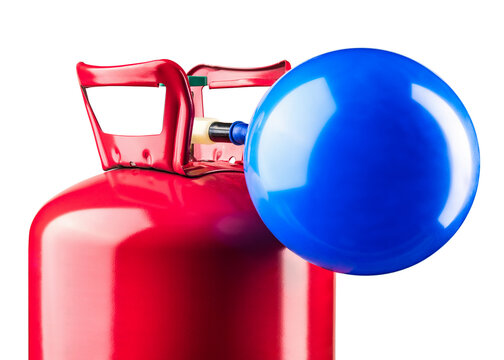
\includegraphics[width=0.3\textwidth,keepaspectratio]{Problem_5/Figs/P5.jpg}
\label{figP5}
\end{figure}
\setcounter{equation}{0}
\begin{center}
    \normalcolor{\textbf{Bài giải}}
\end{center}
Phụt lớp nước lên bề mặt quả bóng. Chỗ nào thủng lỗ sẽ sinh ra bong bóng. 

\ \ 

\textit{Với quan sát thường thức (hoặc từ kiến thức Vật Lý THPT), có thể bạn cũng nhận ra rằng nếu thêm chút xà phòng pha loãng thì bong bóng xuất hiện sẽ càng có kính thước lớn, dễ phát hiện hơn. Bài tập này được lấy cảm hứng từ một bài kiểm tra kỹ thuật thông dụng, và ở trường hợp chúng ta không muốn làm bẩn hệ hay có nước tung tóe vung vãi khắp nơi (như trong phòng thí nghiệm, khi hệ cần kiểm tra đã được đặt trên dụng cụ quan sát), lựa chọn chất lưu tốt hơn sẽ là cồn tinh khiết (ethanol hoặc 2-propanol), do nó không những vẫn có thể tạo ra bong bóng nhỏ kêu lép bép tại vị trí rò, mà còn bốc hơi biến mất rất nhanh.}

\begin{center}
    \normalcolor{------------------------------------------------ HẾT ------------------------------------------------}
\end{center}

\newpage
{ \normalcolor \textbf{Danh sách thành viên tham gia xây dựng [Hướng tới chuyên lý 2024]:}} \\ \vspace{0.5cm}

% \textbf{\textit{Thành Viên tham gia đề xuất các bài tập:}}
\begin{enumerate}
    \item \textbf{Hirrus} (Trưởng nhóm)
    \item \textbf{Colevol}
    \item \textbf{Mino}
    \item \textbf{wan}
    \item \textbf{Khui đạp chai}
    \item \textbf{trees\&streetslights.inc}
    \item \textbf{Carina}
    \item \textbf{LunarEclipse}
\end{enumerate}


\end{document}